\documentclass[fleqn,usenatbib]{mnras}

\usepackage[T1]{fontenc}

\DeclareRobustCommand{\VAN}[3]{#2}
\let\VANthebibliography\thebibliography
\def\thebibliography{\DeclareRobustCommand{\VAN}[3]{##3}\VANthebibliography}


%%%%% AUTHORS - PLACE YOUR OWN PACKAGES HERE %%%%%

% Only include extra packages if you really need them. Common packages are:
\usepackage{graphicx}	% Including figure files
\usepackage{amsmath}	% Advanced maths commands
\usepackage{amssymb}	% Extra maths symbols
\usepackage{xcolor}
\usepackage{tikz}
\usepackage{colortbl}
\usepackage{dsfont}
\usepackage{siunitx}
\usepackage{bm}
\usepackage{caption}
\usepackage{subcaption}

\usetikzlibrary{arrows.meta}


%%%%%%%%%%%%%%%%%%%%%%%%%%%%%%%%%%%%%%%%%%%%%%%%%%

%%%%% AUTHORS - PLACE YOUR OWN COMMANDS HERE %%%%%
\newcommand{\jtd}[1]{ {\bf{\color{red} JTD: #1}} }
\newcommand{\unit}[1]{\bm{\hat{#1}}}

\newcommand{\parens}[1]{\left( #1 \right)}
\newcommand{\brackets}[1]{\left[ #1 \right]}
\newcommand{\quat}[1]{\widetilde{\bm{#1}}}

% Please keep new commands to a minimum, and use \newcommand not \def to avoid
% overwriting existing commands. Example:
%\newcommand{\pcm}{\,cm$^{-2}$}	% per cm-squared

%%%%%%%%%%%%%%%%%%%%%%%%%%%%%%%%%%%%%%%%%%%%%%%%%%

%%%%%%%%%%%%%%%%%%% TITLE PAGE %%%%%%%%%%%%%%%%%%%

\title[Flyby Constraints on Asteroids Interiors]{Constraining the Interiors of Asteroids Through Close Encounters}

% The list of authors, and the short list which is used in the headers.
% If you need two or more lines of authors, add an extra line using \newauthor
\author[Jack T. Dinsmore, Julien de Wit]{
Jack T. Dinsmore,$^{1}$\thanks{E-mail: jtdinsmo@mit.edu}
Julien de Wit$^{2}$
\\
% List of institutions
$^{1}$Department of Physics, Massachusetts Institute of Technology\\
$^{2}$Department of Earth, Atmospheric, and Planetary Science, Massachusetts Institute of Technology
}

% These dates will be filled out by the publisher
\date{Accepted XXX. Received YYY; in original form ZZZ}

% Enter the current year, for the copyright statements etc.
\pubyear{2022}

% Don't change these lines
\begin{document}
\label{firstpage}
\pagerange{\pageref{firstpage}--\pageref{lastpage}}
\maketitle

% Abstract of the paper
\begin{abstract}
  Knowledge of the interior density distribution of an asteroid can reveal its composition and constrain its evolutionary history. However, most asteroid observational techniques are not sensitive to interior properties. We investigate the interior constraints accessible through monitoring variations in angular velocity during a close encounter. We derive the equations of motion for a rigid asteroid's orientation and angular velocity to arbitrary order and use them to generate synthetic angular velocity data for a representative asteroid on a close Earth encounter. Using Markov Chain Monte Carlo fits, we perform injection-retrieval tests on these synthetic data to gain insights into the extent to which interior properties can be constrained. We also perform a sensitivity analysis of such an inversion technique to asteroid parameters (e.g., moment of inertia and initial spin pole direction), observational set-up (e.g., measurement precision and cadence), and mapping models to convert constraints on the density moments to density distributions. We find that high precision in rotational period estimates (order of milliseconds to seconds) are necessary for each cadence, and that large asteroids ($> 100$ m radius) with low perigees ($<20$ Earth radii) are necessary to resolve second-order density moments.
\end{abstract}

% Select between one and six entries from the list of approved keywords.
% Don't make up new ones.
\begin{keywords}
  minor planets, asteroids: general -- methods: data analysis
\end{keywords}

%%%%%%%%%%%%%%%%%%%%%%%%%%%%%%%%%%%%%%%%%%%%%%%%%%

%%%%%%%%%%%%%%%%% BODY OF PAPER %%%%%%%%%%%%%%%%%%

\section{Introduction}

Over the past twenty years, the increase in quantity and quality of sensitive all-sky surveys has prompted the discovery of numerous asteroids. Such advances have been made via ground-based surveys such as the Catalina Sky Survey \cite{larson1998catalina}, Pan-STARRS \cite{kaiser2002pan}, and the Lincoln Near-Earth Asteroid Research project (LINEAR) \cite{stokes2000lincoln}, as well as space-based instruments such as the Wide-field Infrared Survey Explorer (WISE) mission \cite{wright2010wide}. Many of these asteroids are relatively small, but some are kilometre-sized and a few are predicted to closely encounter Earth or other planets in the near future. More encounter candidates are likely to be discovered by new efforts such as the Large-aperture Synoptic Survey Telescope (LSST) \cite{tyson2002large}. Their encounters can then be monitored by global ground-based networks such as the Las Cumbres Observatory (LCO) \cite{brown2013cumbres}. Such ground-based monitoring is typically used to derive the rotation period of an asteroid and its surface properties (see e.g. \cite{10.1093/mnras/stab1252}).

Since the tidal torque acting on an asteroid during an encounter depends on the interior mass distribution, the careful monitoring of angular velocity variations during an encounter also presents a window into the interior properties of asteroids. The gravitational two-body system has
been studied in the context of tidal torque to different orders
and with several different methods \cite{paul88, SCHEERES2000106, ashenberg07, BOUE2009750, HouMar2017}. Further studies showed that the tidal torque, observed through angular velocity perturbations, is sensitive to asteroid interior density distribution \cite{Naidu_2015, Makarov2022ChaosOO, scheeres2004evolution}. However, density distribution features beyond the moment of inertia (MOI) ratios have not yet been extracted for any asteroid encounters. More research is needed to study in what cases these effects are observable, and what
factors generally inhibit observation of these new features. 

Angular velocity perturbations have been observed and
used to extract asteroid properties in several cases, including
for the 2013 encounter of (367943) Duende with Earth \cite{MOSKOVITZ2020113519, benson2020spin}, and asteroid
binaries (3905) Doppler and (617) Patroclus \cite{DESCAMPS2020113726, BERTHIER2020113990}. Orbital and physical properties, including MOI ratios have also been extracted for 99942 Apophis, which will closely encounter Earth in 2029 \cite{yu2014numerical, hirabayashi2021finite, valvano2022apophis, Lee2022Apophis}. It seems pivotal to augment previous work on the affect of tidal torque on Apophis' angular velocity \cite{souchay2014rotational, souchay2018changes} so that upcoming observations may constrain these properties and thus improve our predictions.

We address this community need by developing a methodology to translate (1) time series of asteroid angular velocity data into constraints on density moments and (2) constraints on density moments into constraints on an asteroid's density distribution. Other techniques, such as measurement of tidal distortion \cite{RICHARDSON199847}, impact or seismometry experiments \cite{RICHARDSON2005325}, or gradiometry \cite{carroll2018tidal}, may additionally constrain the density distribution. In section \ref{sec:methods}, we introduce the analytical and numerical fundamentals of this methodology. There, we describe a simulation used to integrate the equations of motion and produce synthetic data of angular velocity over time, followed by a Markov Chain Monte Carlo (MCMC) fit process which  extracts density moments from the fit data. We note that these equations fo motion for an asteroid equation are novel and designed to be computationally efficient and valid to arbitrary order. We then describe three methods to generate full density distributions from the density moments. In section \ref{sec:results}, we present the results of a series of injection-retrieval tests demonstrating the extent to which the properties of an asteroid chosen to generate synthetic spin data can be retrieved via our methodology. Finally, in section \ref{sec:discussion}, we assess the sensitivity of these constraints to various physical, observational, and methodological parameters to provide guidance for monitoring upcoming close encounters. We also test the density distribution extraction methods on several sample asteroids.





\section{Methods}
\label{sec:methods}

The only properties of an asteroid's density moments that affect tidal torque interactions are its ``density moments,'' defined here as
\begin{equation}
  K_{\ell m} = \frac{a_\mathcal{A}^{2-\ell}}{I_\mathcal{A}} \int_\mathcal{A} d^3 r \rho_\mathcal{A}(\bm r) R_{\ell m}(\bm r).
  \label{eqn:klm}
\end{equation}
These are complex, unitless quantities. $\rho_\mathcal{A}(\bm r)$ is the asteroid density distribution and $R_{\ell m}$ are the regular solid spherical harmonics (see appendix \ref{app:eom} for details). The integral is computed over the entire asteroid mass, denoted $\mathcal{A}$. $I_\mathcal{A}$ denotes a MOI scale defined as 
\begin{equation}
  I_\mathcal{A} = \int_\mathcal{A} d^3 r \rho_\mathcal{A}(\bm r) r^2
  \label{eqn:ia}
\end{equation}
while $a_\mathcal{A}$ is the length scale
\begin{equation}
  a_\mathcal{A}^2 = \frac{1}{V_\mathcal{A}} \int_\mathcal{A} d^3 r r^2
  \label{eqn:aa}
\end{equation}
where $V_\mathcal{A}$ is the asteroid volume. We call these MOI and length scales in part because they obey $I_\mathcal{A} = \mu_\mathcal{A} a_\mathcal{A}^2$ where $\mu_\mathcal{A}$ is the mass of the asteroid for uniform asteroids. Note that $a_\mathcal{A}$ is a function only of the surface of the asteroid, so that $a_\mathcal{A}$ is known if the surface is observed.

The tidal torque experienced by an asteroid is 
\begin{equation}
  \begin{split}
  \bm \tau = & G\frac{I_\mathcal{A}I_\mathcal{B}}{2 a_\mathcal{A}^2a_\mathcal{B}^2}\left[\sum_{\ell m} a_\mathcal{B}^\ell J_{\ell m} \sum_{\ell' m'}a_\mathcal{A}^{\ell'}S^*_{\ell+\ell', m + m'} (\bm D) (-1)^{\ell'}\right.\\
  \times & \left.\sum_{m''=-\ell'}^{\ell'} \sqrt{\frac{(\ell'-m'')!(\ell'+m'')!}{(\ell'-m')!(\ell'+m')!}}  \mathcal{D}^{\ell'}_{m'm''}(\alpha, \beta, \gamma)^* \right. \\
  \times & \Big((i\unit x - \unit y)(\ell'-m''+1)K_{\ell',m''-1} \\
  & +(i\unit x+\unit y)(\ell'+m''+1)K_{\ell',m''+1}+2im''\unit z K_{\ell'm''}\Big) \Bigg],
  \end{split}
  \label{eqn:tidal-torque}
\end{equation}
where $\bm D$ is the position of the asteroid; $\alpha$, $\beta$, and $\gamma$ are $z-y-z$ Euler angles expressing the orientation of the asteroid; $S_{\ell m}$ are the irregular solid spherical harmonics; and $\mu_\mathcal{B}$ and $a_\mathcal{B}$ are the mass and radius of the central body while $J_{\ell m}$ are the density moments of the central body, with the $a_\text{bulk}$ and $a_\text{surf}$ of equation \ref{eqn:klm} replaced by $a_\mathcal{B}$. Equation \ref{eqn:tidal-torque} is derived in appendix \ref{app:eom}, assuming a rigid asteroid and no distant third-body perturbations. 

Since it is the angular acceleration of the asteroid that is observable, rather than the torque applied, we also compute the MOI of the asteroid around the principal axes: 
\begin{equation}
  \begin{split}
    I_x &= \frac{2}{3} I_\mathcal{A} \parens{K_{20} - 6 K_{22} + 1}\\
    I_y &= \frac{2}{3} I_\mathcal{A} \parens{K_{20} + 6 K_{22} + 1}\\
    I_z &= \frac{2}{3} I_\mathcal{A} \parens{-2K_{20} + 1}.
  \end{split}
  \label{eqn:moi}
\end{equation}

The angular acceleration of the asteroid is proportional to $\bm \tau / I$ (equation \ref{eqn:omega-eom}), such that the $I_\mathcal{A}$ factor of equation \ref{eqn:tidal-torque} is canceled out. Thus, the observables do not depend explicitly on $I_\mathcal{A}$, nor on the asteroid mass.

Throughout the paper, we refer to the ``inertial frame'' (the frame in which the orbit is fixed) and the ``body-fixed frame'' (the frame in which the asteroid is fixed and in which $K_{\ell m}$, $I_\mathcal{A}$, and $a_\mathcal{A}$ are computed), which are also defined in appendix \ref{app:eom}.

\subsection{Simulation design}
\label{sec:sim}

We built a publicly accessible, custom simulation in C++ to produce time series of angular velocity data during a close encounter with a central body. This simulation requires as initial data (1) the orbital parameters of the asteroid $r_p$ (perigee distance) and $v_\infty$ (hyperbolic excess velocity); (2) the cadence of angular velocity observation $\Delta t$; (3) the central body moments $J_{\ell m}$, mass $\mu_\mathcal{B}$, and radius $a_\mathcal{B}$; (4) the initial asteroid angular velocity in the inertial frame $\bm \Omega_0$; (5) the asteroid length $a_\mathcal{A}$ and (6) the asteroid's density moments $K_{\ell m}$ and initial Euler angle $\gamma_0$. All parameters except (6) are assumed to be known to high accuracy. For example, $\bm \Omega_0$ could be extracted from pre-encounter light-curve data and $a_\text{surf}$ from a model for the asteroid's surface using radar.

We assume for simplicity that the asteroid is initially not tumbling, though this assumption can be relaxed. We assume a short-axis rotation mode such that energy of the asteroid's rotation is minimized. This sets $\beta = 0$ and we can further choose $\alpha = 0$. Only the Euler angle $\gamma_0$ is necessary to provide initial data for the simulation.

We begin our simulation at $D = 10 r_p$, with velocity predicted by Kepler's laws given by the orbital parameters. Since the leading order of the equations of motion is $\ell' = 2, \ell = 0$, this corresponds roughly to a torque of $10^{-3}$ times the maximum torque at perigee. Unless otherwise indicated, the simulation is terminated at $D=10 r_p$ as well.

With the simulation inputs specified, the equations of motion are integrated via the Runge-Kutta fourth order method, with a variable time step
\begin{equation}
  dt = dt_\text{min} + 10^{-3}(dt_\text{max} - dt_\text{min}) \brackets{\parens{\frac{D}{r_p}}^3 - 1}.
\end{equation}
The parameters $dt_\text{max}$ and $dt_\text{min}$ (20 and 10 seconds respectively) were chosen such that the numerical integration error was $\sim$100 times the floating point error, and that neighbouring values of $K_{\ell m}$ yielded significantly different spin pole data compared to floating point error. The data used to choose this $dt$ was obtained using the reference asteroid configuration, described in appendix \ref{app:reference-configs}.



\subsection{Uncertainty model}
\label{sec:uncertainty}

To add noise to data generated via the above simulation, we use the following uncertainty model. Each asteroid spin vector $\bm \Omega$ is assumed to be uncorrelated with other spin vectors, and we model uncertainty in the orientation and in the period as also uncorrelated. Consider a true spin vector $\bm \Omega^*$. For the sake of description, we work in coordinates in which $\bm \Omega^* \parallel \unit z$. Then, expressing the observed spin vector $\bm \Omega$ in spherical coordinates, we draw the polar angle from a normal distribution with standard deviation $\sigma_\theta$ centred on zero and the azimuthal angle from a uniform distribution. We also draw the ratio $\Omega/\Omega^*$ from a log-normal distribution centred on one, with width $\sigma_P / P$, where $P = 2\pi \Omega$ is the period of the asteroid. Explicitly, the probability density function (PDF) of $\rho$ is 
\begin{equation}
  P(\rho) = \frac{1}{\rho\sqrt{2\pi (\sigma_P / P)^2}} \exp\parens{-\frac{\ln^2\rho}{2(\sigma_P / P)^2}}.
\end{equation}
See figure \ref{fig:uncertainty-model} for an illustration of the uncertainty model. A log normal distribution is chosen such that $\rho > 0$, but since $\sigma_\rho \ll 1$ typically in our analysis, $P(\rho)$ is approximately Gaussian.

\begin{figure}
  \centering
  \begin{tikzpicture}
  \draw[-{Latex[length=3mm]}] (0, 0) -- (-4, 0) node[anchor=east] {$\unit X$};
  \draw[-{Latex[length=3mm]}] (0, 0) -- (1, -1.5) node[anchor=west] {$\unit Y$};
  \draw[-{Latex[length=3mm]}] (0, 0) -- (0, 4) node[anchor=south] {$\unit Z$};

  \draw[line width=0.5mm, -{Latex[length=3mm]}] (0, 0) -- (-3, 3) node[anchor=south] {$\bm \Omega^*$};
  \draw[dashed] (-3, -2) -- (-3, 3);
  \draw[dashed] (-3, -2) -- (0, 0);

  \draw[-{Latex[length=3mm]}] (0, 0) -- (-1.25, 3.35) node[anchor=south west] {$\bm \Omega$};
  \draw[rotate around={-50:(-3,3)}] (-3,3) ellipse (1.4 and 2);
  \draw (-3, 3) arc (110:93:6);
  \draw (-2, 3.5) node[anchor=center] {$\theta$};
  \draw (-0.5, 2.5) node[anchor=center] {$\rho \Omega^*$};

  \end{tikzpicture}
  \caption{Diagram in the inertial frame of the uncertainty model used to define the probability that the true spin vector $\bm \Omega^*$ should be observed as $\bm \Omega$. The parameter $\theta$ is drawn from a Gaussian with width $\sigma_\theta$, and $\rho$ is drawn from a log normal distribution with width $\sigma_\rho$.}
  \label{fig:uncertainty-model}
\end{figure}

The log likelihood resulting from this uncertainty model is (excluding additive constants)
\begin{equation}
  \begin{split}
  \ln \mathcal{L} = -\frac{1}{2}\sum_{i = 0}\Bigg[&\frac{\cos^{-1} (\bm \Omega_i^* \cdot \bm \Omega_i/(\Omega_i^* \Omega_i))^2}{\sigma_\theta^2}\\
  &+\frac{\ln \parens{\Omega_i /\Omega_i^*}^2}{(\sigma_P / P)^2} + 2\ln\frac{\Omega_i}{\Omega_i^*}\Bigg].
  \end{split}
  \label{eqn:log-likelihood}
\end{equation}
where $\Omega_i$ is the $i$th spin vector in the data set.

This model was chosen because it separates spin pole and period uncertainty. Therefore, if one is more precisely determined by measurement, $\sigma_\theta$ and $\sigma_P / P$ can be adjusted separately in accordance.





\subsection{Extracting density moments from spin data}
\label{sec:fit}
Given synthetic data, an Affine Invariant MCMC Ensemble sampler was used to generate PPDs from flat priors. We use the Python implementation \texttt{emcee} \cite{foreman2013emcee}. Our parameters were $\gamma_0$, $K_{20}$, $K_{22}$, and $K_{3m}$ (10 in total), and were bounded by $|\gamma_0| < \pi/4$, and bounds on $K_{2 m}$ given in equation \ref{eqn:parameter-bounds}. Note that $\gamma_0$ is degenerate with $\gamma_0 + \pi/2$ because both of these align the asteroid principal axes with the body-fixed axes. The other bounds were $|K_{3m}| < 1$. In general, spin data is most sensitive to $\gamma_0$ and $K_{2m}$, which we call the ``first-order parameters.'' We call $K_{3m}$ the ``second-order parameters.''

The MCMC was determined to converge when the fractional change in autocorrelation time (computed every 100 iterations) was one percent, and the number of iterations computed so far was more than 100 times the autocorrelation time. The MCMC fit also was set to terminate if more than $10^5$ iterations were run, but this only occurred for fits in which the data quality was low, leading to degeneracies between the second order parameters ($K_{3 m}$). This degeneracy could be removed by only fitting $K_{2m}$ instead. About $10^4$ iterations was often sufficient, which generally consumed about 7 hours of computation time on a super computer running 16 threads on 8 cores.

Before the MCMC was run, local minima in the likelihood were found via the Nelder-Mead algorithm implemented in \texttt{scipy} \cite{Gao2012}. Generally, only one local minimum existed, except when $K_{22}=0$ in which case rotational symmetry caused multiple values of $\gamma_0$ to be degenerate. Ensemble walkers were initialized near this local minimum, distributed by a Gaussian approximation of the likelihood, as determined via the Hessian of the likelihood at the minimum. Due to the high sensitivity of the angular velocity data to density moments, the minimization procedure sometimes failed to isolate the minimum likelihood. Therefore, a simpler simulation without the $K_{3m}$ terms of equation \ref{eqn:tidal-torque} was first used to minimize likelihood as a function of the first-order parameters $\gamma_0$ and $K_{2m}$, and then the full simulation was used to find the second-order parameters $K_{3m}$ with the first-order parameters fixed.

To further ensure convergence, we minimized with respect to data truncated after perigee at double the perigee distance. This cut-off was manually chosen. The minimum was then further refined by minimizing based on the full data, with the previous minimum as the initial estimate.


\subsection{Density distributon constraints}
\label{sec:density-distro}

The asteroid density distribution $\rho_\mathcal{A}(\bm r)$ is not uniquely constrained via tidal torque interactions because only the density moments $K_{\ell m}$ contribute to equation \ref{eqn:tidal-torque}. For example, since the mass of the asteroid is unconstrained, $\rho_\mathcal{A}(\bm r)$ cannot be determined on an absolute scale. However, by making sufficient assumptions about the density distribution, we can nevertheless extract fluctuations in $\rho_\mathcal{A}(\bm r)$ across the asteroid from $K_{\ell m}$. To best understand the potential density distribution of an asteroid, an ensemble of models with differing assumptions is desired, so that common traits across the models can be identified. To this end, we throughly outline two possible models and discuss two more in appendix \ref{app:other-models}.

We assume that the asteroid's surface is known in the inertial frame from radar data. Since the asteroid tumbles during the encounter, we also assume that the center of mass of the asteroid is extracted.  However, the density moments which are extracted from flyby data are known instead in the body-fixed frame.

We rotate the known surface of the asteroid to a new frame called the ``hybrid frame'' by translating such that the known center of mass is at the origin, then rotating such that $\Omega_0$ points in the $+\unit z_\text{hybrid}$ direction and $\unit Y$ points in the $\unit Y_\text{hybrid}$ direction. Since $\Omega_0$ is exact, the surface in this hybrid frame is known exactly. The hybrid frame differs from the body-fixed frame only by a rotation around $\unit z_\text{hybrid}$ of $\gamma_0$. Such rotations affect density moments via 
\begin{equation}
  K_{\ell m}^\mathrm{hybrid} = e^{-im\gamma_0}K_{\ell m}^\mathrm{body-fixed}.
  \label{eqn:body-fixed-to-hybrid}
\end{equation}
by equation \ref{eqn:ylm-rotation}. Thus, uncertainty on $K_{\ell m}^\mathrm{body-fixed}$ (obtained from the encounter data) can be translated to uncertainty in $K_{\ell m}^\mathrm{hybrid}$. Henceforth, we will operate only in the hybrid frame and suppress the label.

When the $K_{3m}$ are extracted, 15 moments are known (excluding $K_{00}$). Since the asteroid mass cannot be determiend by this analysis, it is convenient to additionally set the mass equal to its volume, so that the average density is one and thus the extracted densities can be interpreted as ratios of $\rho / \rho_\text{avg}$. Three more moments are redundant with the center of mass, such that only twelve finite elements are free. In cases where $\gamma_0$ is known very accurately such that the correction imposed by equation \ref{eqn:body-fixed-to-hybrid} is very small, it is numerically favourable not to impose this equation on $K_{2m}$. In this case, the three orientation constraints that set $K_{21}=\Im K_{22} = 0$ carry over to the hybrid frame so that there are nine degrees of freedom (DOF). Since $\gamma_0$ is precisely known for all cases studied in this paper, we will always study this case. We also place additional constraints that $0.25 < \rho < 3$ to ensure realistic densities.

To extract a density distribution, we use another MCMC given one of the two parametrizations of density distributions discussed below. The prior is set to be flat and nonzero for all configurations that obey the $0.25 < \rho < 3$ constraint. The likelihood used is set equal to the multivariate-Gaussian approximation of the posterior distribution for $K_{\ell m}$, extracted from flyby data. Otherwise, the MCMC parameters chosen were identical to those discussed in section \ref{sec:fit}. We also present two further models in appendix \ref{app:more-models} which are viable substitutes for the following two models but are not used in the main text.



\subsubsection{Finite element model}

Given values of $K_{\ell m}^\mathrm{body-fixed}$ and their uncertainties extracted from encounter data, there are many ways to extract a density distribution. Here, we outline a method termed the ``finite element'' model. We divide the asteroid into $N$ finite elements of uniform density and use the density $\rho_i$ of each as parameters. The four constraints imposed by the known mass and center of mass of the asteroid (seven with $K_{21}$ and $\Im K_{22}$ are also fixed) are used to constrain some of these $\rho_i$. The constrained densities are easily computed since the asteroid mass $\mu_\mathcal{A}$ and the product $I_\mathcal{A}K_{\ell m}$ are both linear functions of $\rho_i$. Because $K_{\ell m} = 0$ implies that $I_\mathcal{A}K_{\ell m} = 0$, computing the constrained densities is simply a matrix inversion.

The size and location of the elements must be chosen before extracting their densities. Best results generally require elements of equal size to be chosen. To remove the dependence on this choice, density distributions for many distinct element layouts can be extracted and the density of each point in the asteroid can be randomly sampled from any of these solutions to yield estimates for the mean density and uncertainty in density at each point.

The value of $N$ must be carefully chosen, since it embodies a balance between the precision and accuracy of the resulting distribution. If $N$ is set equal to the number of data points, an accurate solution is  guaranteed, but uncertainties are inflated. If $N$ is chosen lower, the choice of element layout might exclude a distribution that exactly matches $K_{\ell m}$, but uncertainties are diminished due to less redundancy in the model. An analysis of which value of $N$ is appropriate for our purposes is given in section \ref{sec:dof-scan}.

\subsubsection{Lumpy model}

A drawback of the finite element model is that the generated density distribution might not be representative of the asteroid if the elements are not optimally placed. We therefore describe an alternate model, which includes the positions of the elements as parameters at the cost of larger elements and therefore lower resolution. We call this model the ``lumpy'' model.

Suppose the asteroid is formed of $N$ constant-density, possibly overlapping ``lumps,'' enclosed within a constant-density substrate whose surface is visible to observers. The lumps and the substrate are described by the mass added to the substrate by a lump $\mu_i$, the position of its center of mass $\bm r_i$ (relative to the asteroid's center of mass), its density moments $K_{\ell m}^{(i)}$, and its length scale $a_i$. Here, $i$ denotes the index of the lump where the substrate is $i=0$.  We do not need to include $I_i$ as a free parameter because these lumps have constant density, so that $I_i = \mu_i a_i^2$. Furthermore, by requiring that a lump's density moments be computed relative to the center of mass of the lump, we have $K_{1m} = 0$.

The translation rules of spherical harmonics give that the asteroid properties in the hybrid frame are
\begin{equation}
  \begin{aligned}
    K_{\ell m} = &\brackets{\sum_{i=0}^N \frac{a_i^2 + r_i^2}
    {a_\mathcal{A}^2}\mu_i}^{-1} \\
    &\times \brackets{\sum_{i=0}^N \sum_{\ell' m'}\mu_i
    \frac{a_i^{\ell'}}{a_\mathcal{A}^\ell}
    R_{\ell - \ell', m - m'}(\bm r_i)K_{\ell' m'}^{(i)}} \\
  \end{aligned}
\end{equation}
where the sum limits are $0 \leq l' \leq l$ and $-\ell' \leq m' \leq \ell'$. We also have total mass and center of mass constraints:
\begin{equation}
  \mu_\mathcal{A} = \sum_{i=0}^N \mu_i,  \qquad 0 = \sum_{i=0}^N \mu_i \bm r_i.
\end{equation}
Additional constraints can be imposed on $K_{\ell m}^{(i)}$ if desired. For example, we can require that the lumps be ellipsoids, so that $K_{3 m}^{(i)} = 0$. Additional rotational symmetries also constrain $K$, with the most extreme case being that spherical lumps have $K_{\ell m} = 0$ for $\ell > 0$. However, $K_{00}=1$ is guaranteed by definition, meaning that each spherical lump has only five DOF ($a_i$, $\mu_i$, and $\bm r_i$). The substrate has one degree of freedom, since only $\mu_0$ is unknown. Thus, this lumpy model has $5N - 3$ total DOF. Again, the choice of $N$ affects the accuracy and uncertainty of the model results, which is discussed in section \ref{sec:density-compare}.



\section{Results}
\label{sec:results}

To demonstrate our interior-probing methodology, we provide a full density distribution retrieval applied to synthetic data for the asymmetric reference asteroid. We first introduce the retrieval capabilities regarding density moments, then we turn to the constraints that can be derived reliably on the density distribution. For both level of information retrieval, we find that the results are consistent with the properties used to generate the synthetic data.

\subsection{Density moments}
\label{sec:example-fit}
\begin{figure}
  \centering
  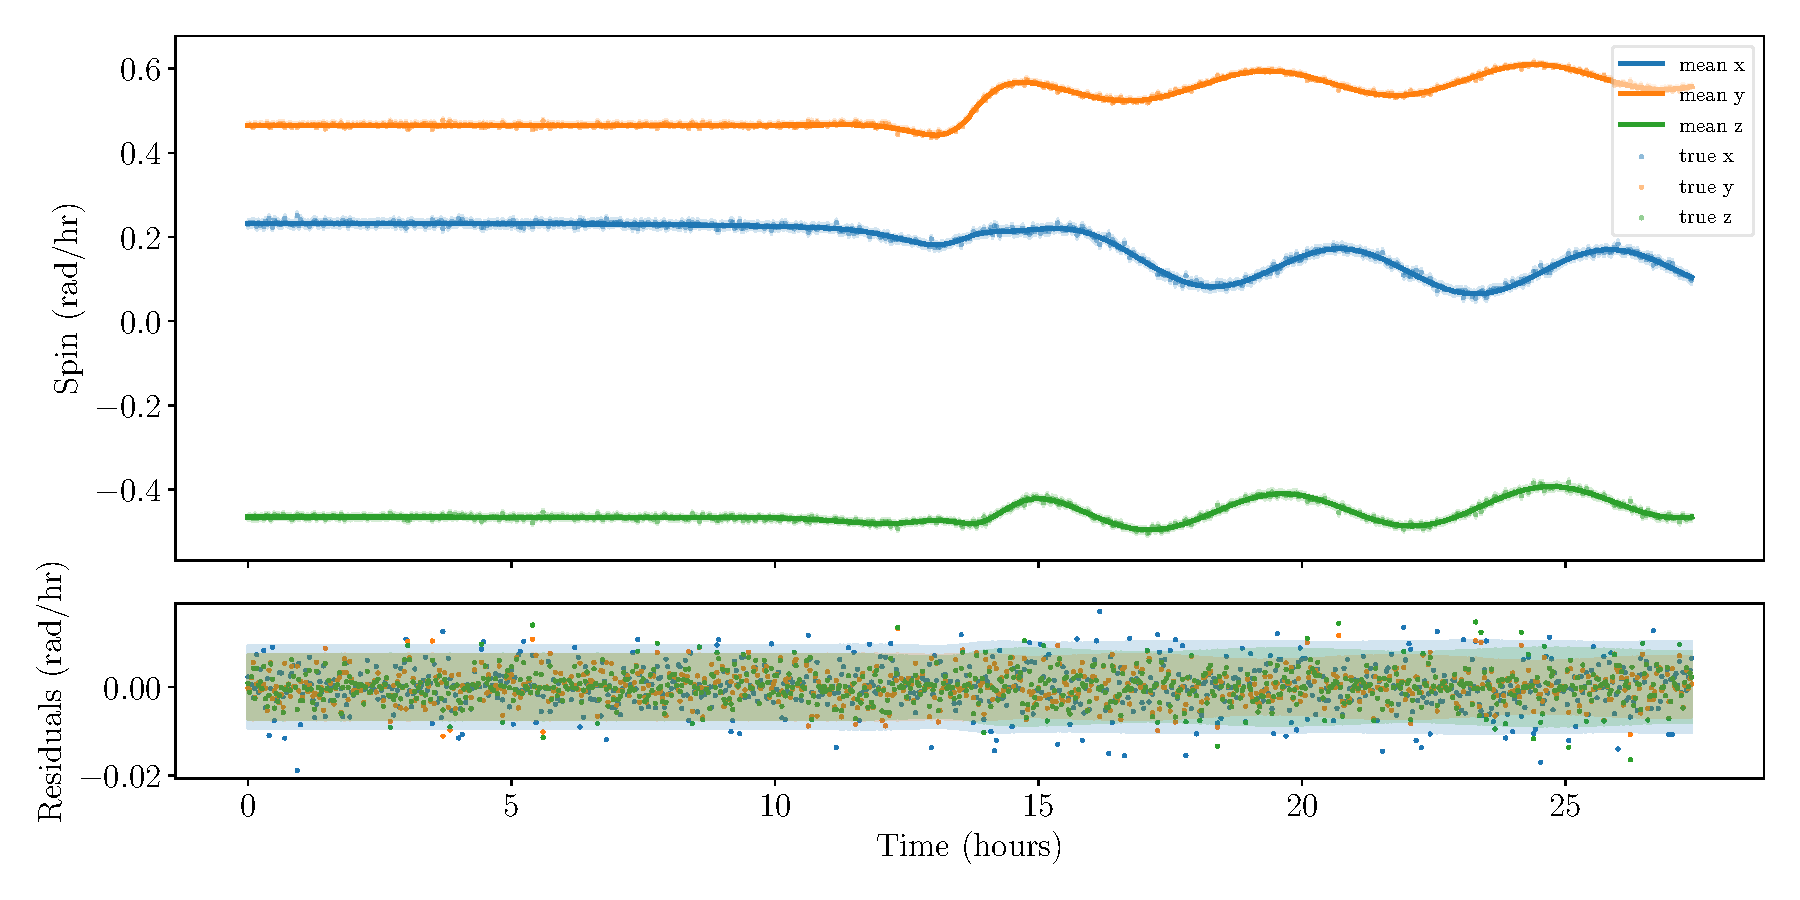
\includegraphics[width=\linewidth]{figs/example-residuals.pdf}
  \caption{Data, best-fitting results, and residuals for a fit to synthetic data simulated for an asymmetric reference asteroid. Uncertainty bands are also shown. The best fit results appear consistent with the data.}
  \label{fig:example-residuals}
\end{figure}

\begin{figure*}
  \centering
  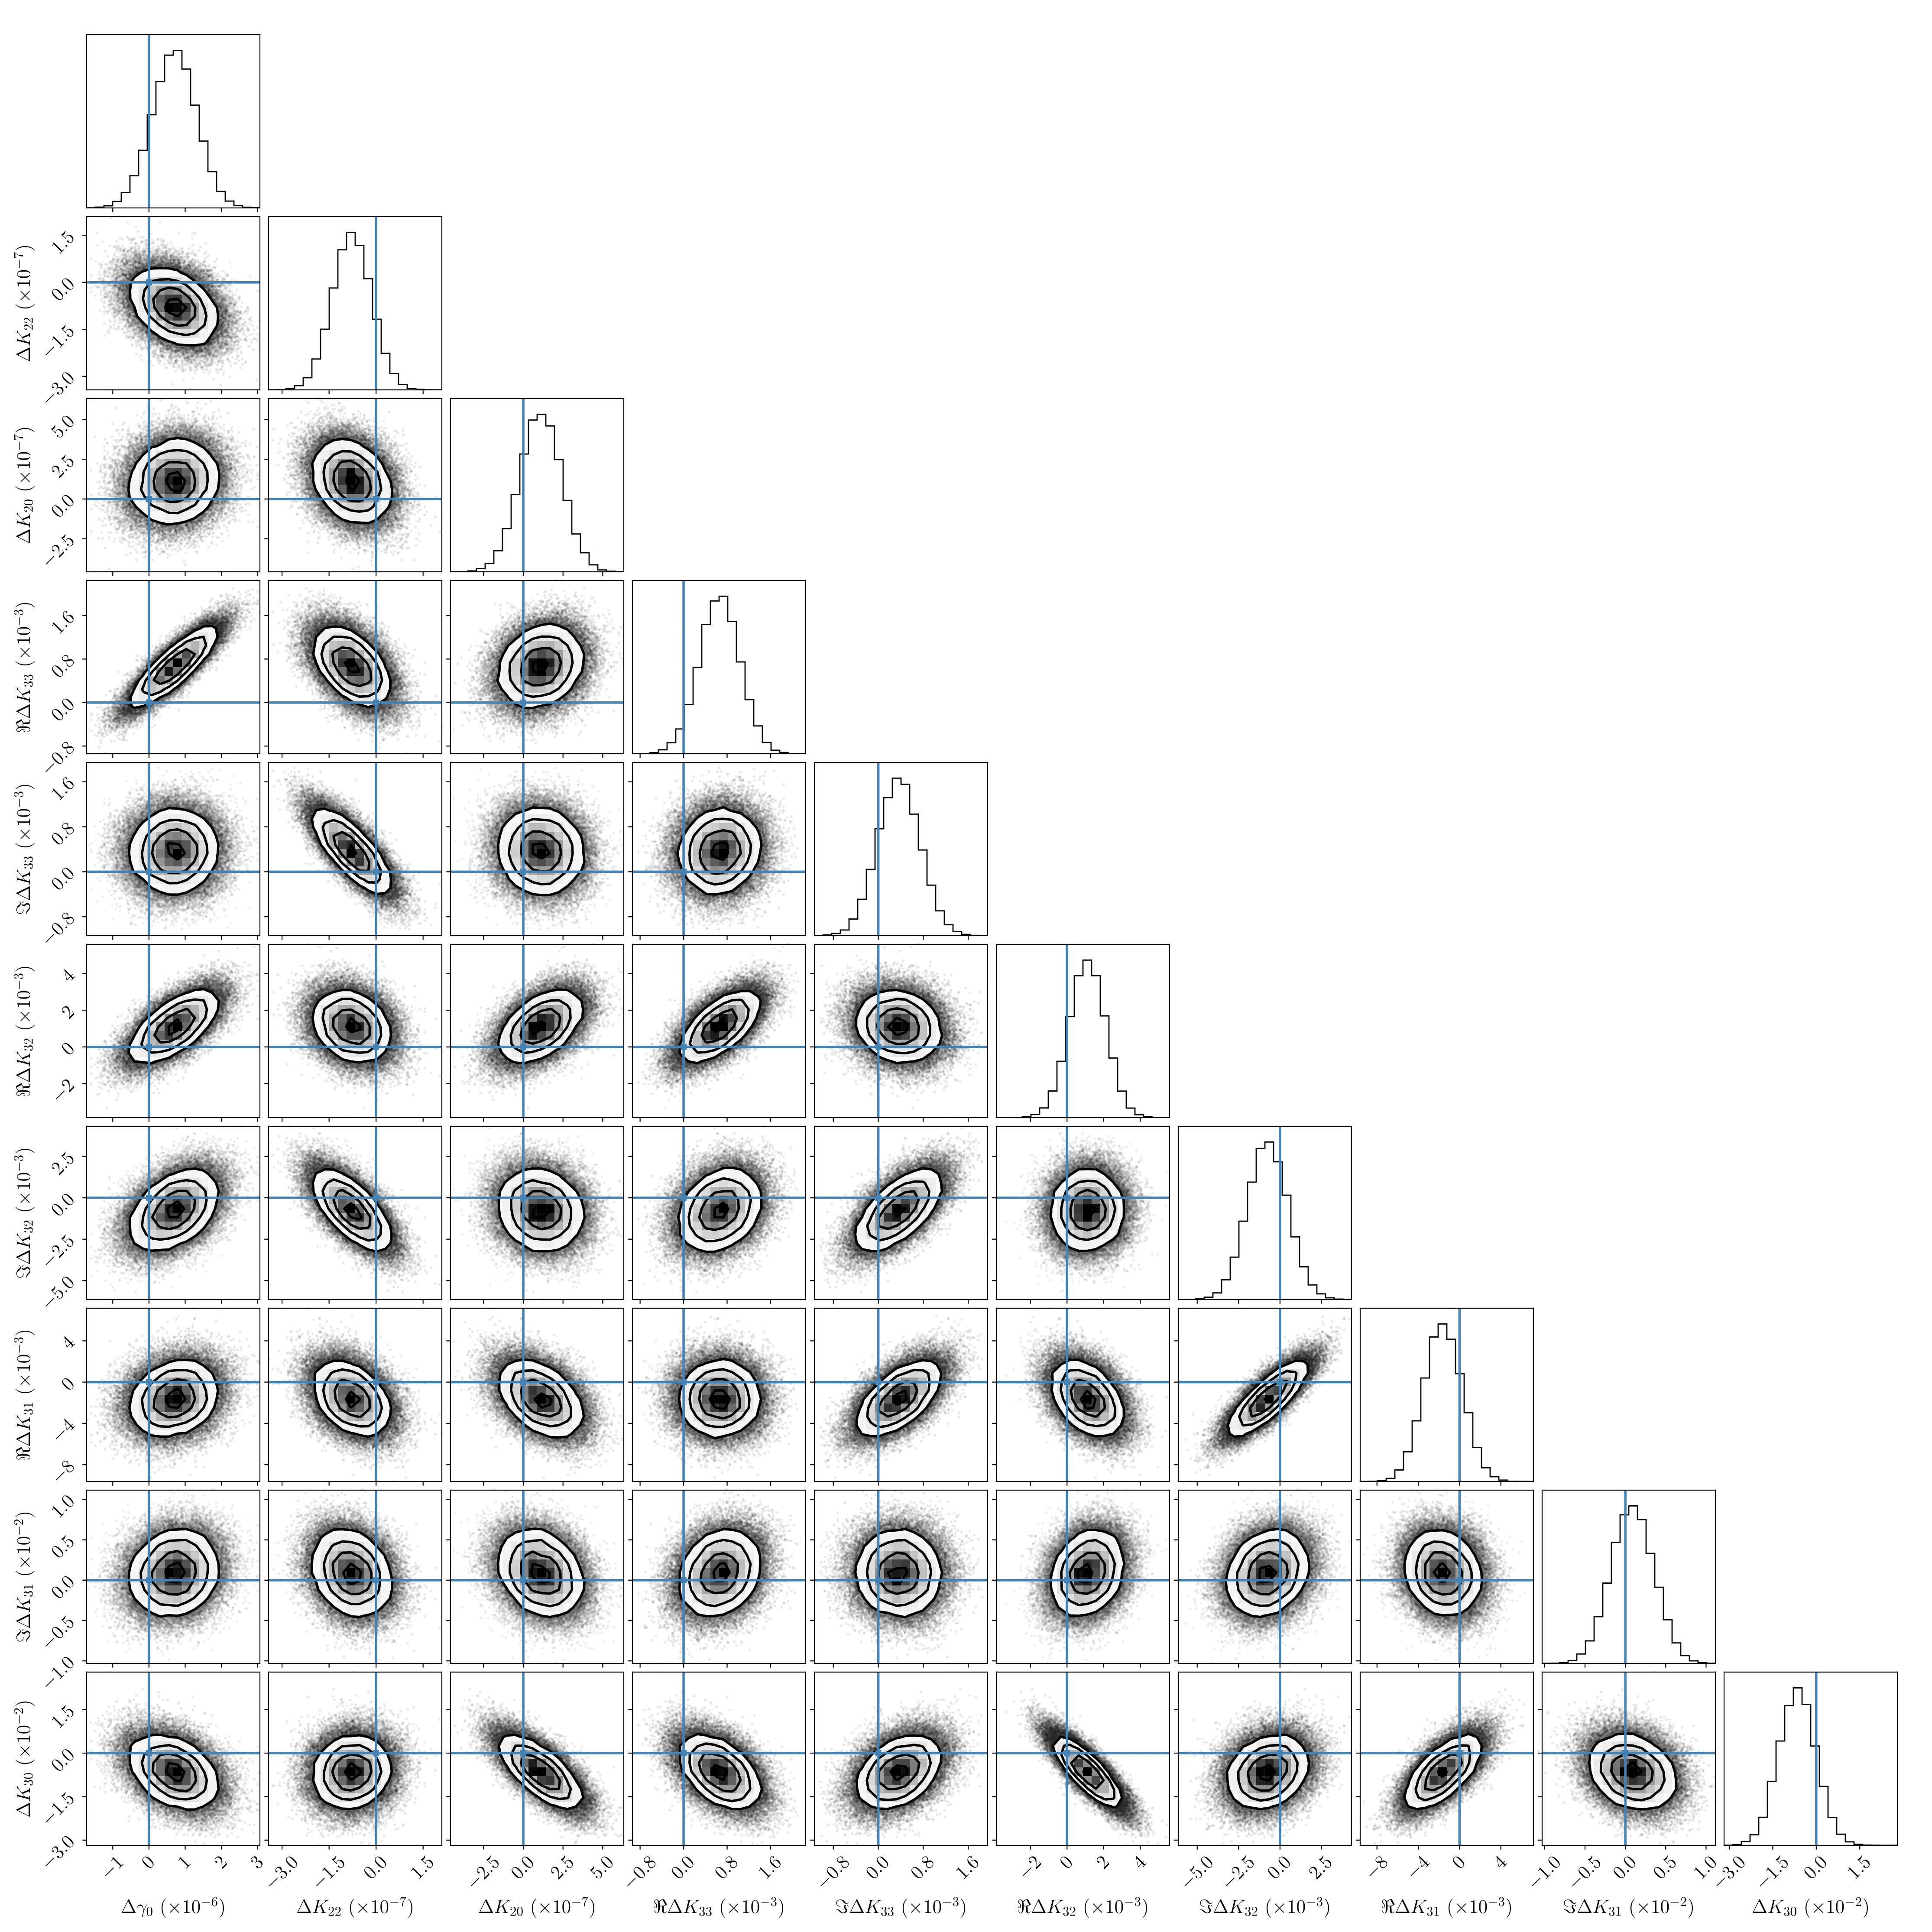
\includegraphics[width=0.85\textwidth]{figs/example-corner.png}
  \caption{PPDs extracted from synthetic encounter data for the asymmetric reference asteroid. Samples from the MCMC fit are shown as individual points, and the contours enclose 1, 2, and 3$\sigma$ confidence regions. True values are shown as blue lines. PPDs are Gaussian and show no degeneracies.}
  \label{fig:example-corner}
\end{figure*}

Figure \ref{fig:example-residuals} shows our synthetic spin data. The best-fitting model is overlaid in the top panel and residuals are shown the bottom panel. Uncertainties are plotted on the residuals corresponding to the square root of the diagonal entries of the covariance matrix (correlations not included). The fit results are clearly consistent with the data. This figure is also instructing in revealing which points in the data set are most informative. The at-perigee data is irregular and reveals information about the density moments, and the post-perigee data shows torque-free tumbling behaviour which constrains $K_{2m}$ via the moment of inertia ratios, and also indirectly sheds light on the at-perigee data by constraining the rotational velocity the asteroid must have had when leaving the perigee.

Figure \ref{fig:example-corner} shows a corner plot of the PPDs of the ten parameters (namely $\gamma_0$ and $K_{\ell m}$ for $\ell \leq 3$), marginalized to functions of one (histograms) or two (contours) variables. The true parameters are shown as lines. Note that the true parameters usually lie within 1 or 2$\sigma$ of the $\Delta K_{\ell m} = 0$, where $\Delta K_{\ell m}$ is the difference between the posterior $K_{\ell m}$ and the true $K_{\ell m}$. The PPDs are generally Gaussian and sometimes show correlation between parameters, but no continuous degeneracy occurs. We performed 48 independent minimizations of the likelihood before the MCMC fit began, each with an initial point chosen randomly in the parameter space. All converged to the same minimum, demonstrating that the model lacks discrete degeneracy as well.



\subsection{Density distribution}
\label{sec:asym-density}

Density moments of the kind described above were extracted for the asymmetric and symmetric reference asteroids. The finite element model was then used to extract density distributions from these moments, and propagate uncertainties. Five DOF were used rather than the maximum possible number of nine, and 20 different finite element layouts were used to generate sample density distributions to avoid dependence on the manually-chosen layout. The resulting density distributions and uncertainties are displayed in figure \ref{fig:uniform}.
\begin{figure*}
  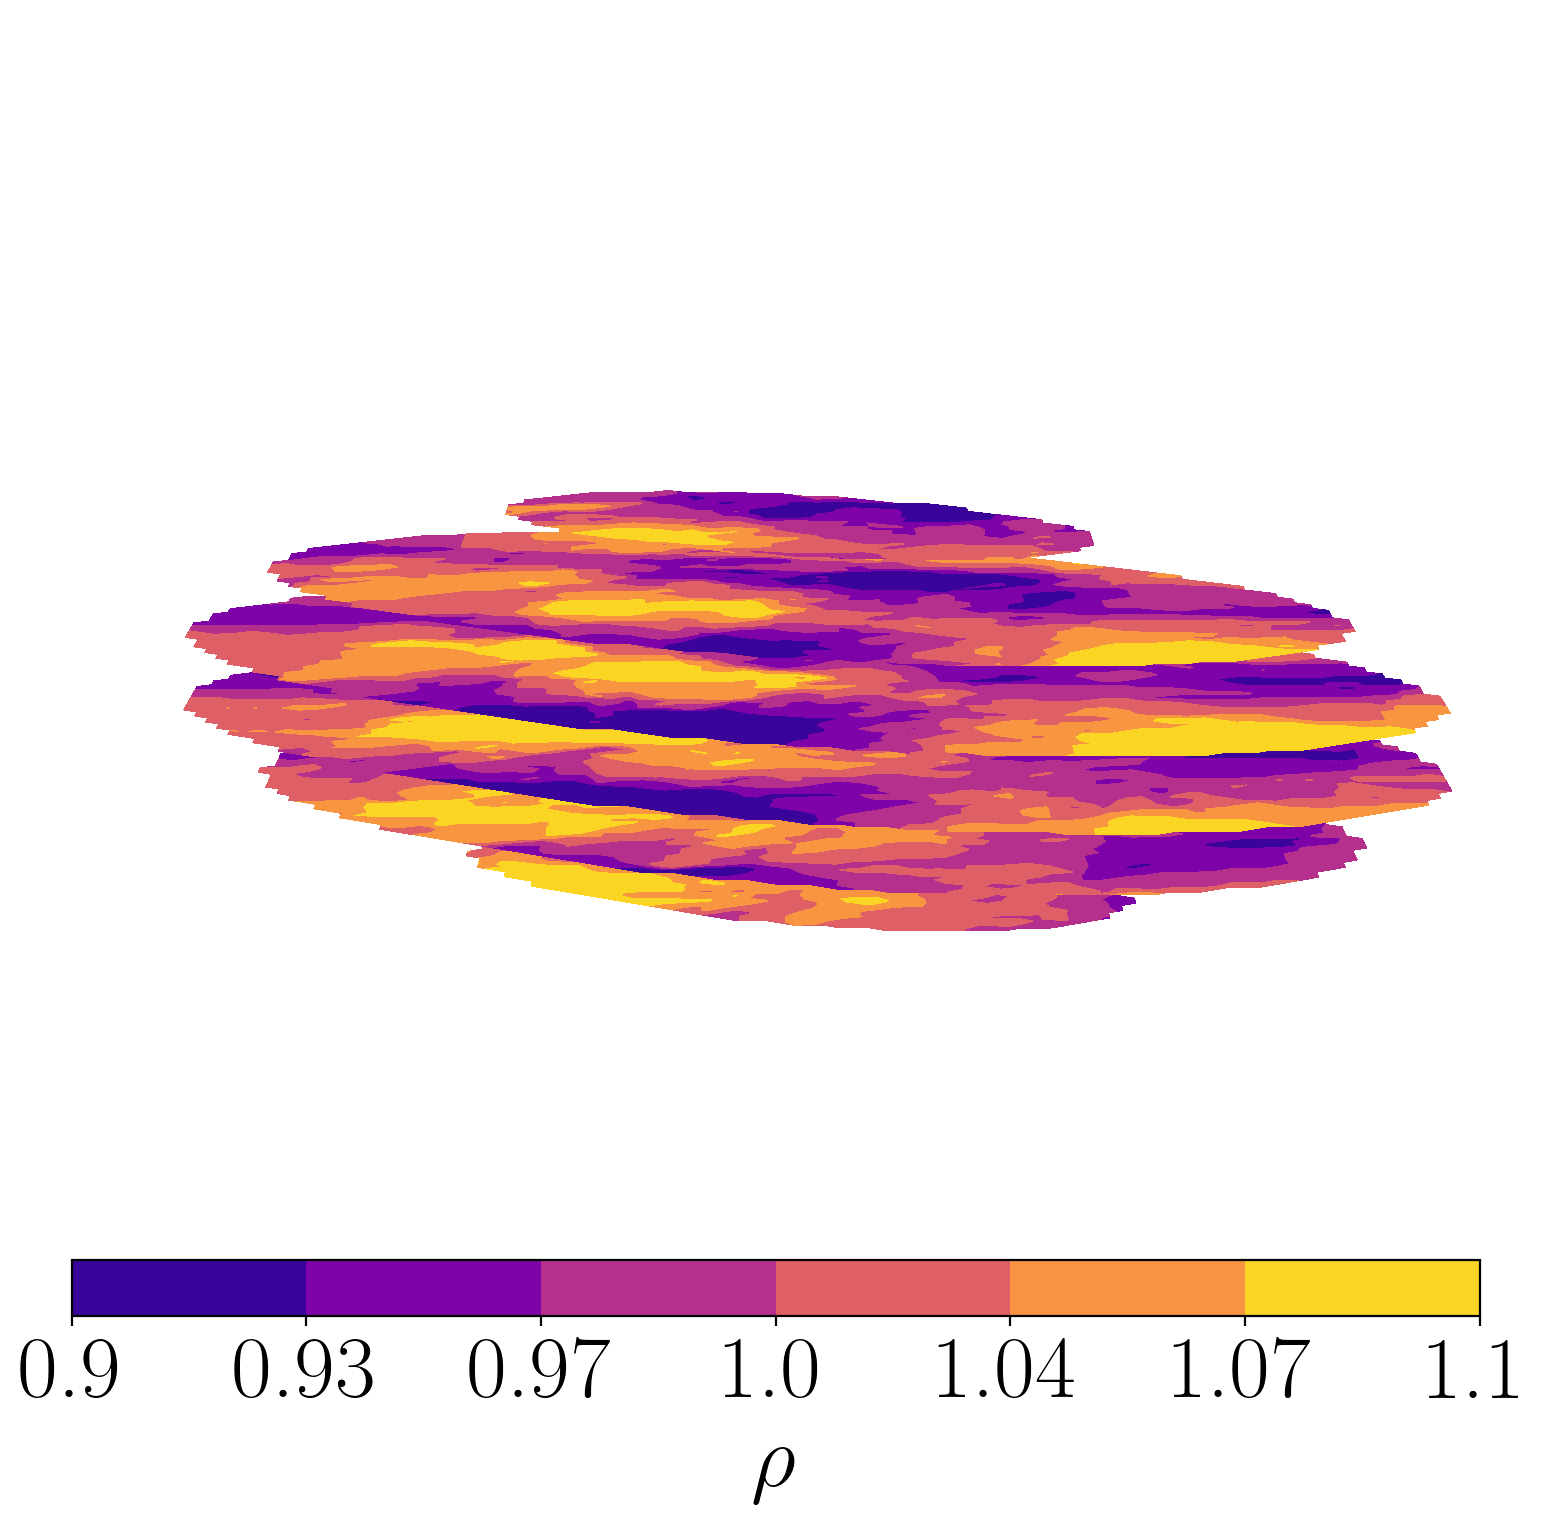
\includegraphics[width=0.24\linewidth]{figs/asym-fe-d}\hfill
  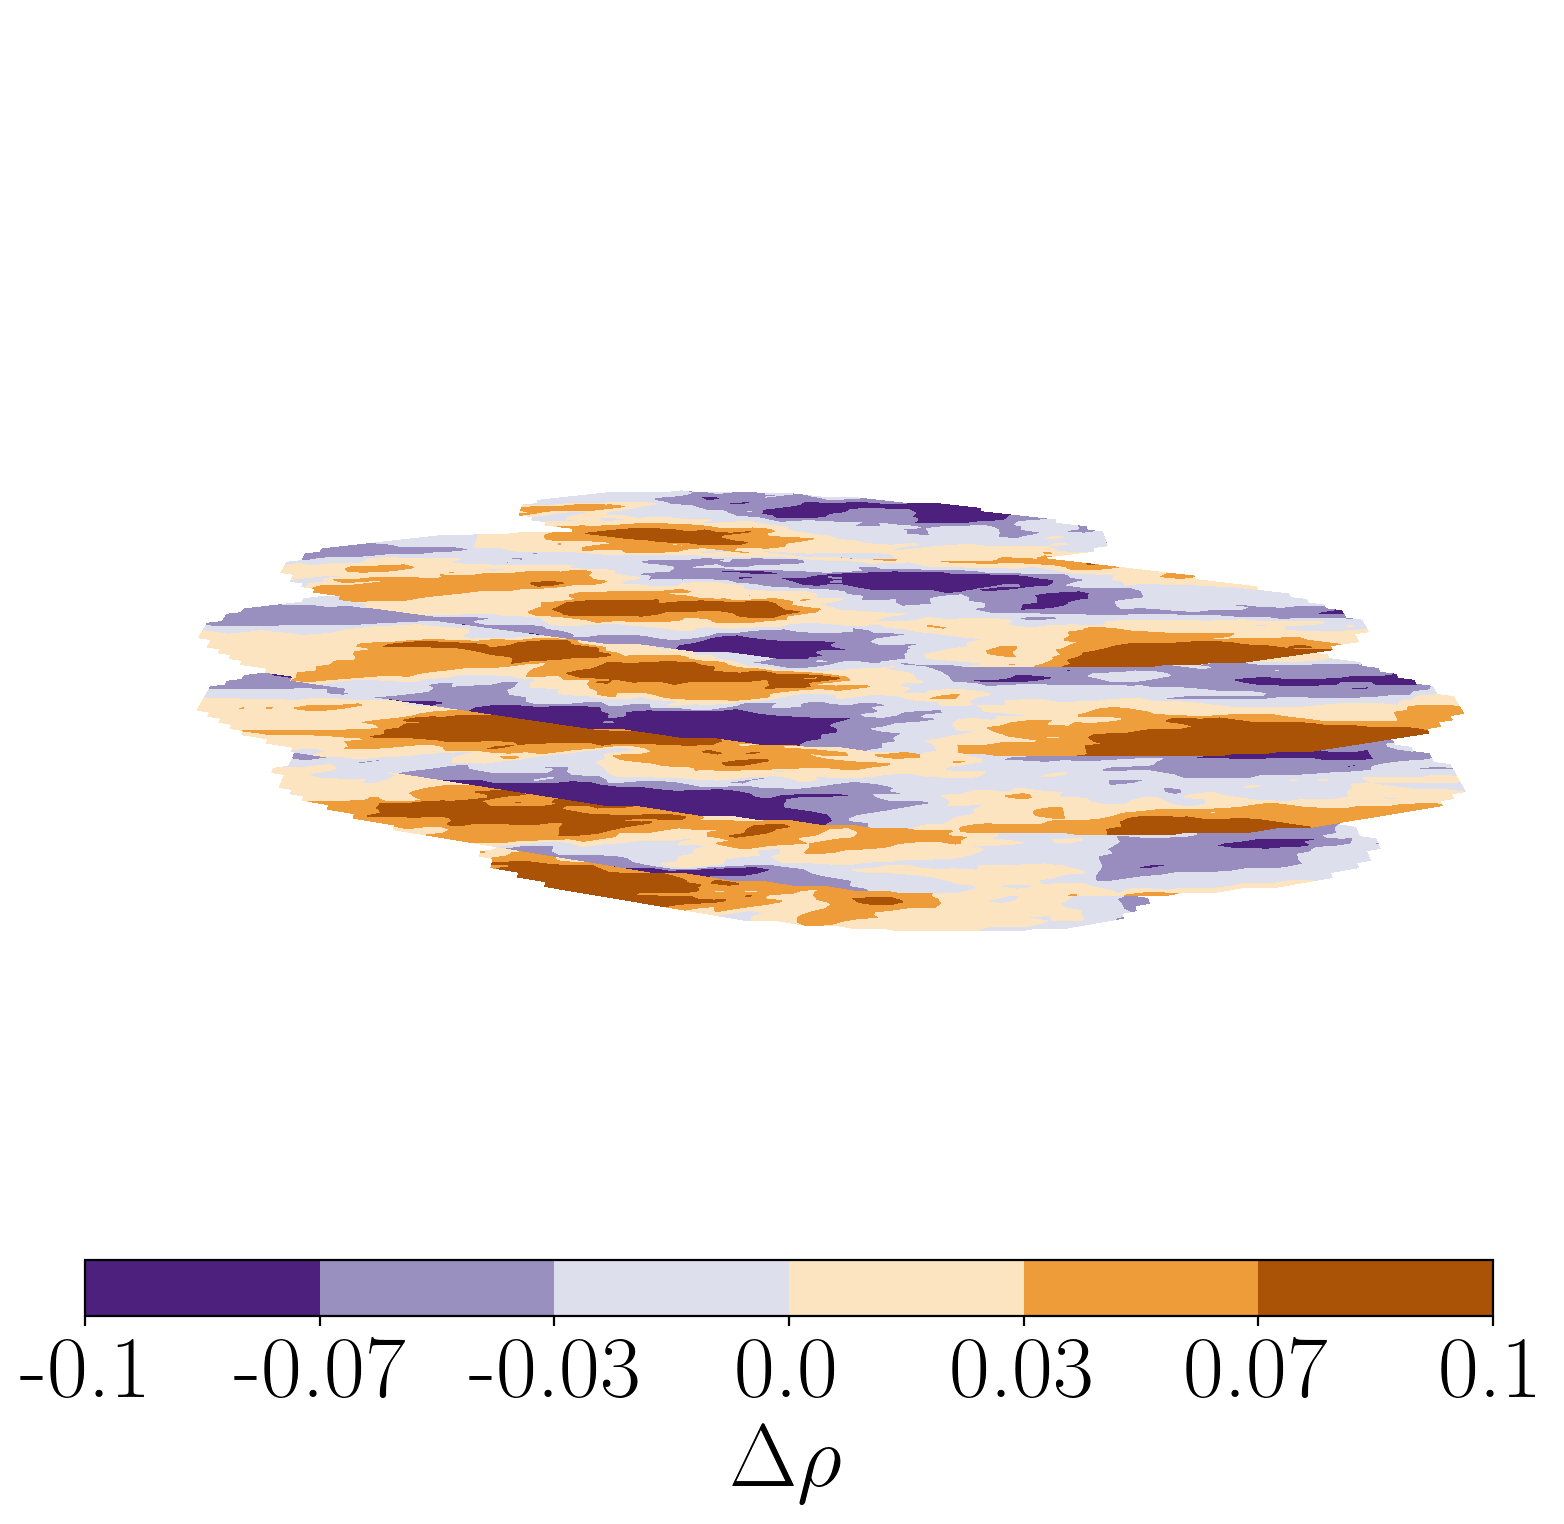
\includegraphics[width=0.24\linewidth]{figs/asym-fe-s}\hfill
  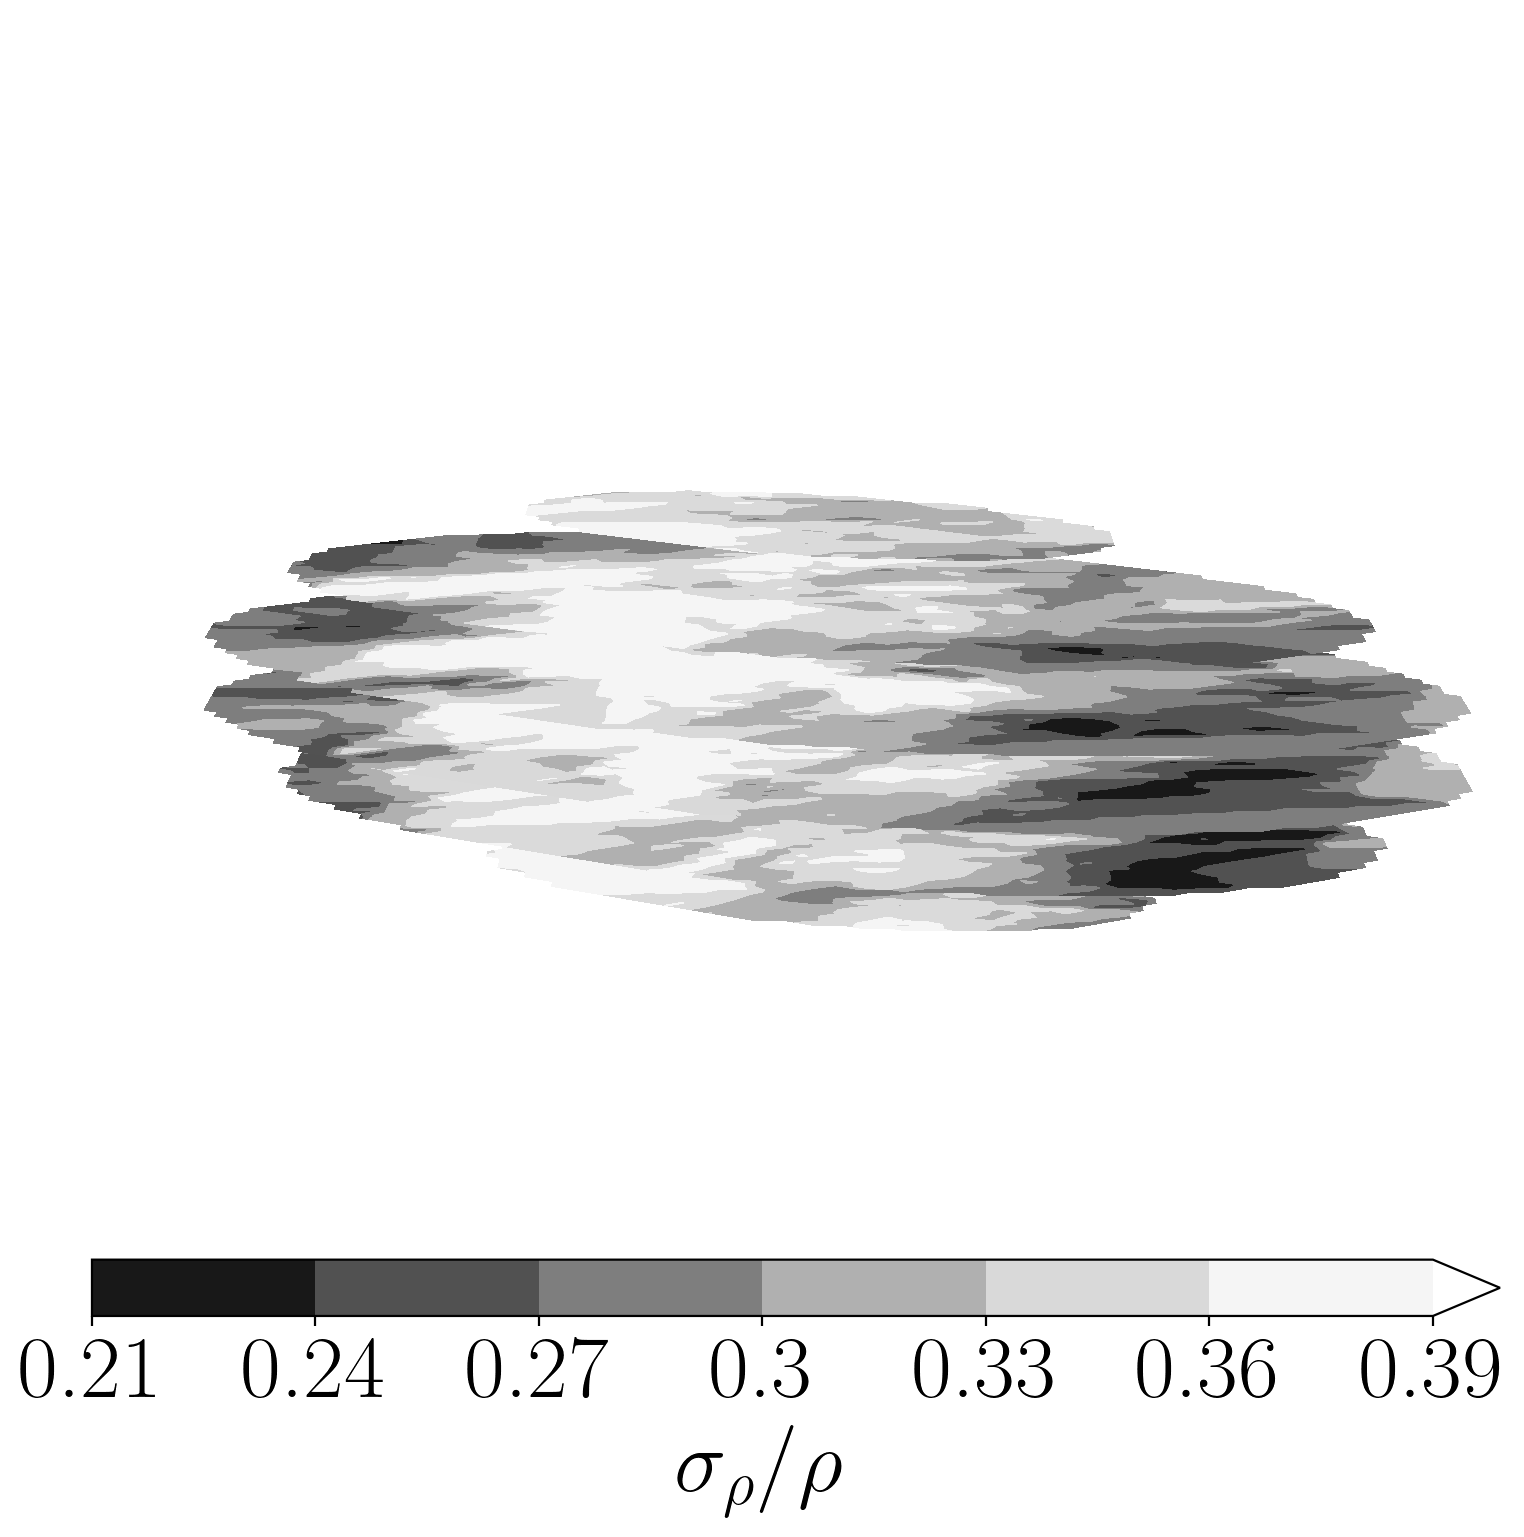
\includegraphics[width=0.24\linewidth]{figs/asym-fe-u}\hfill
  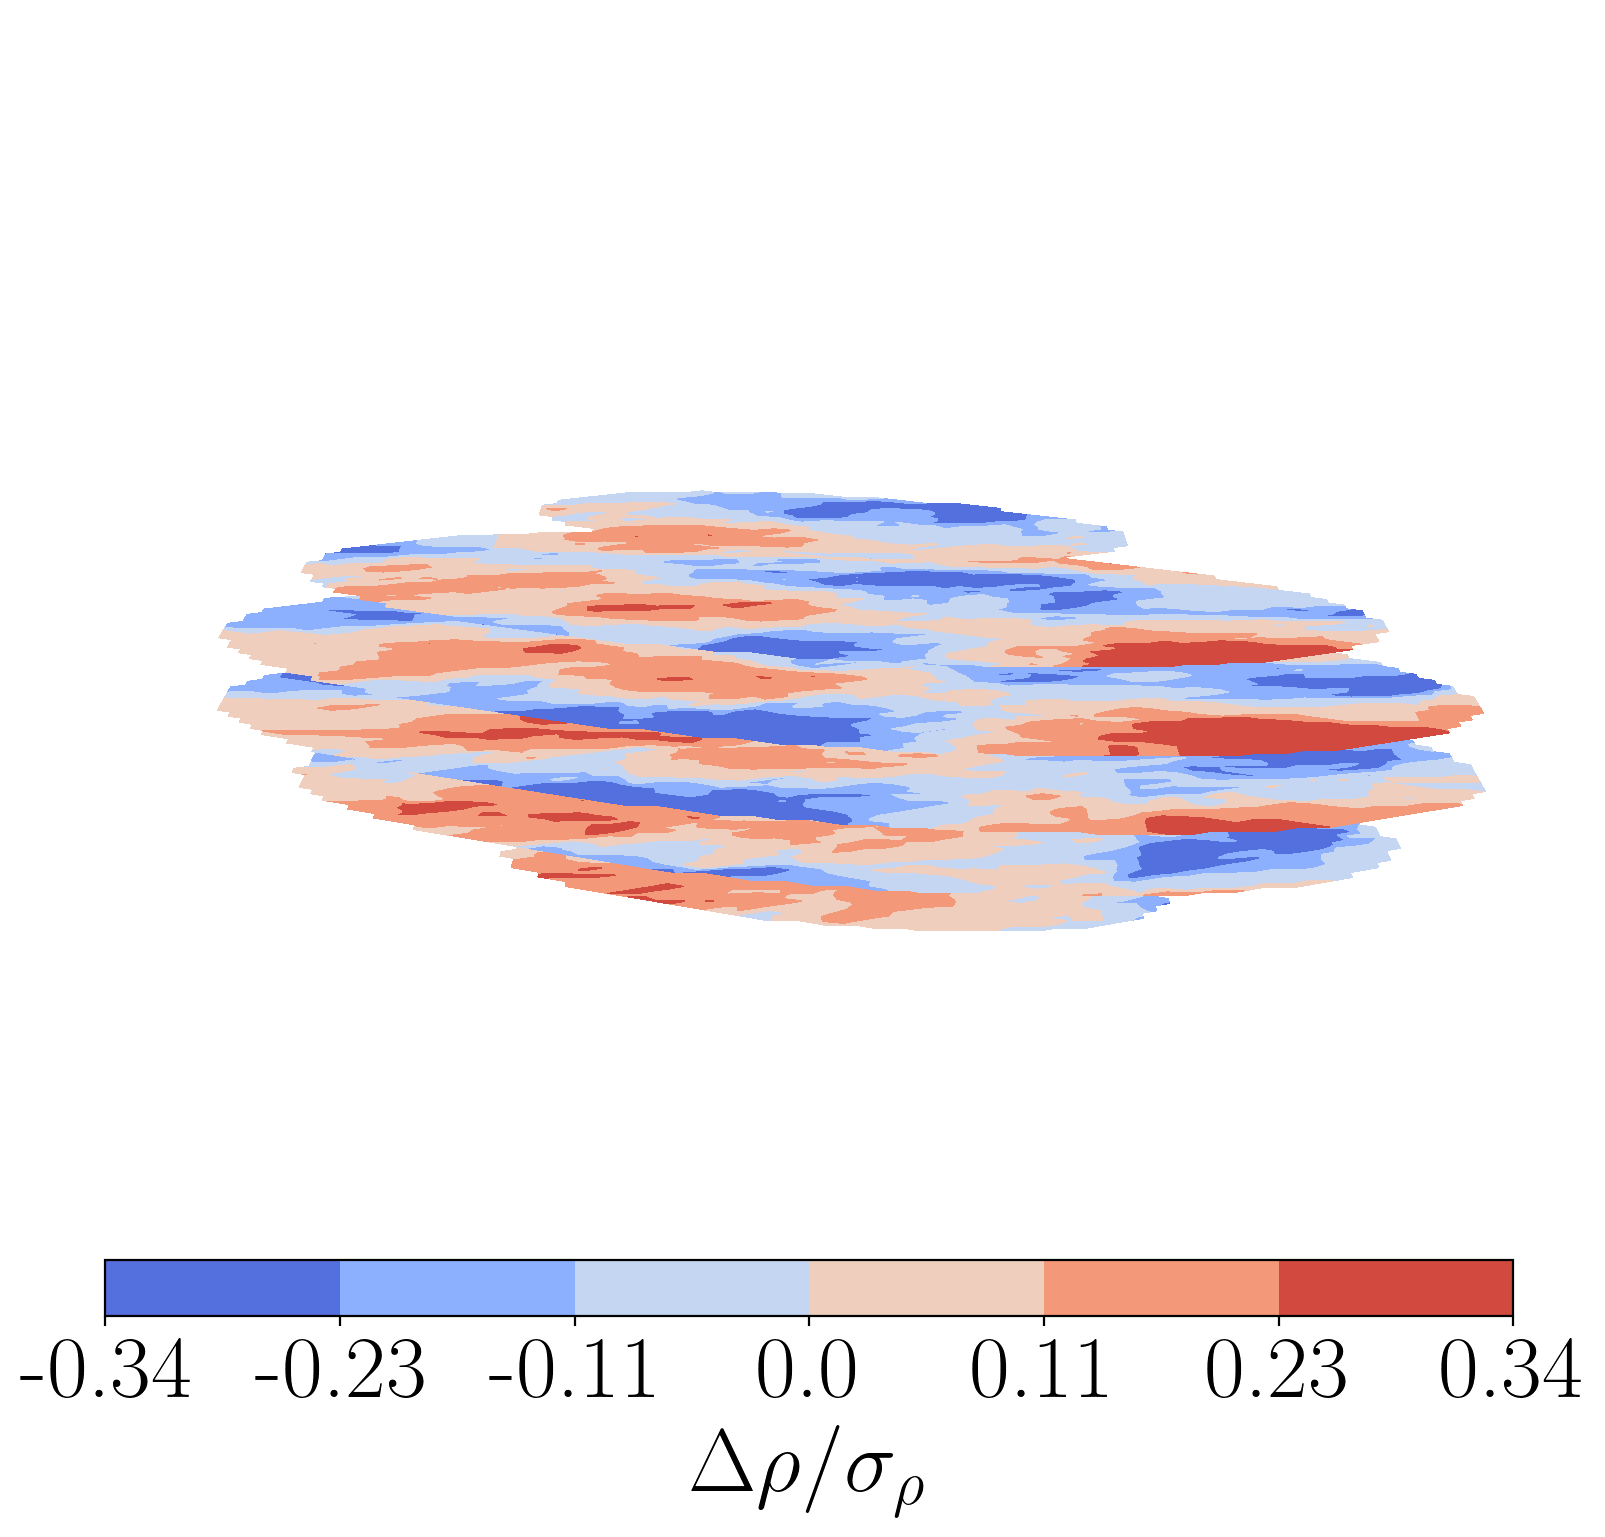
\includegraphics[width=0.24\linewidth]{figs/asym-fe-r}

  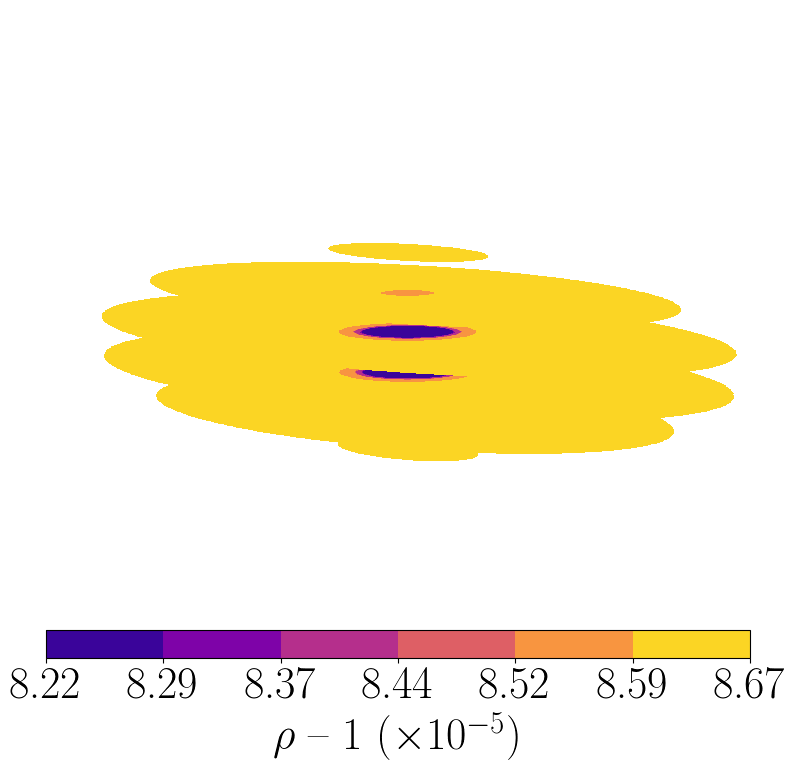
\includegraphics[width=0.24\linewidth]{figs/asym-l-d}\hfill
  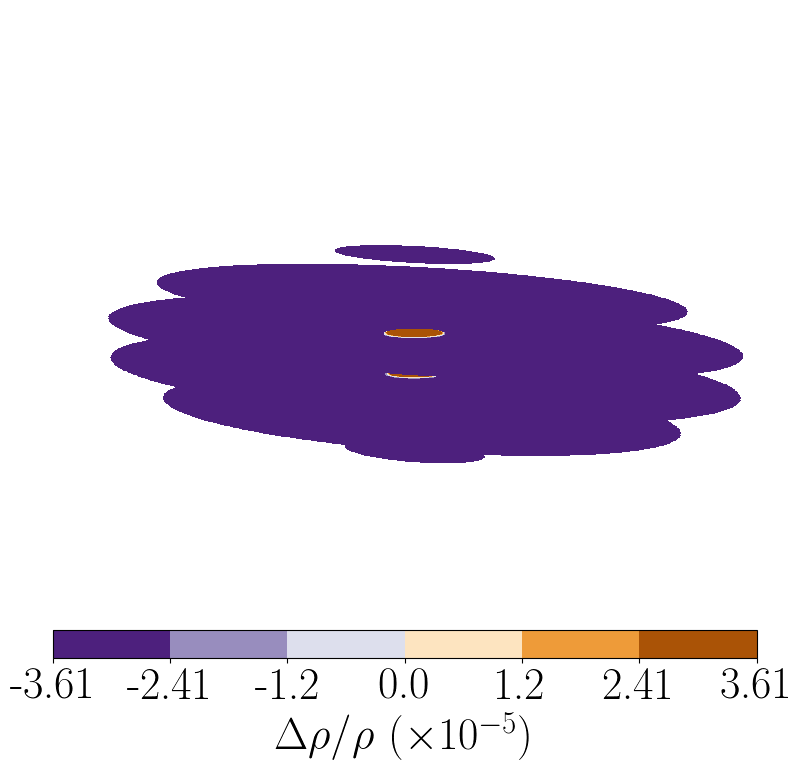
\includegraphics[width=0.24\linewidth]{figs/asym-l-s}\hfill
  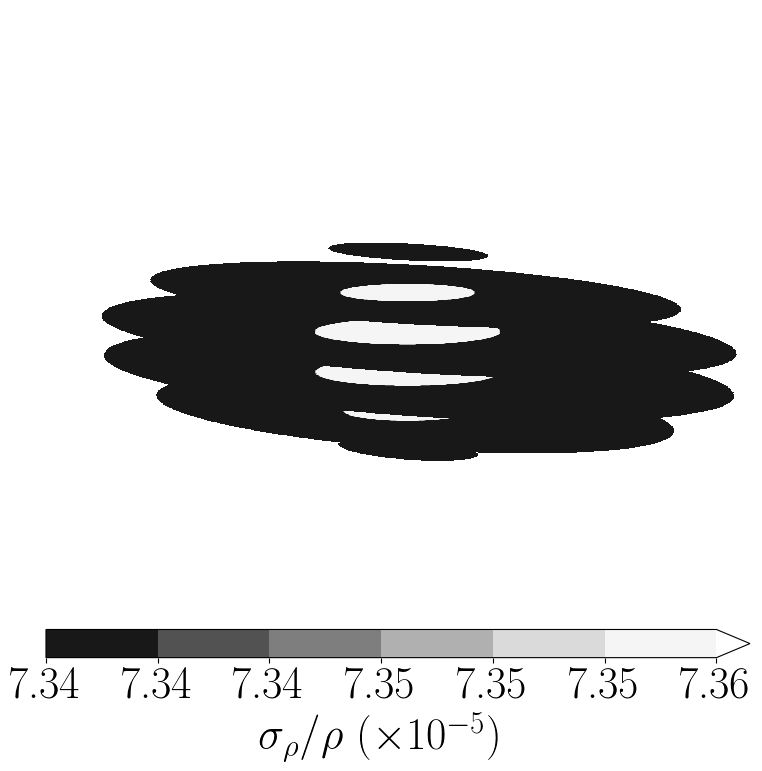
\includegraphics[width=0.24\linewidth]{figs/asym-l-u}\hfill
  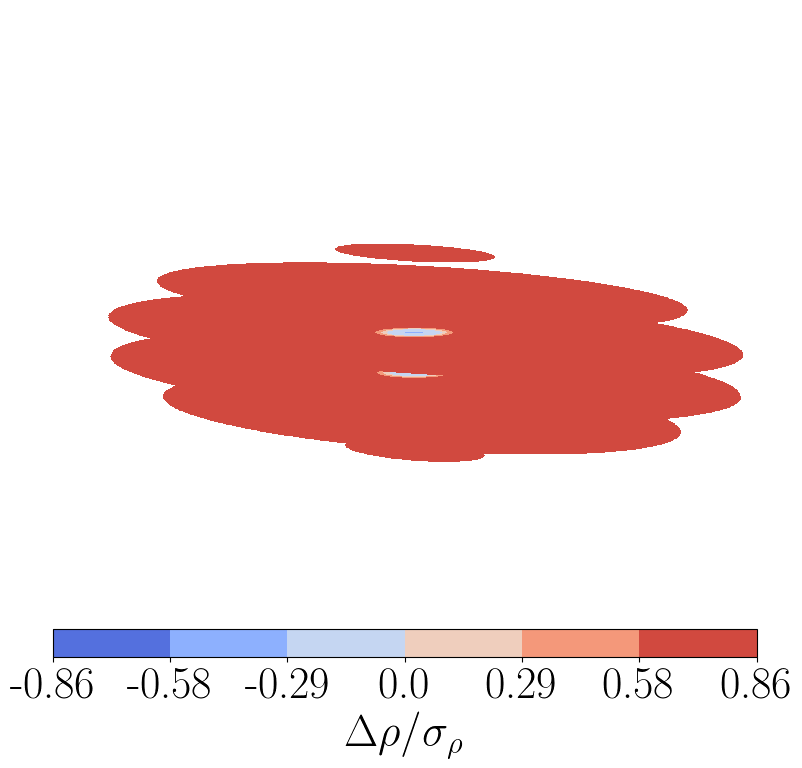
\includegraphics[width=0.24\linewidth]{figs/asym-l-r}

  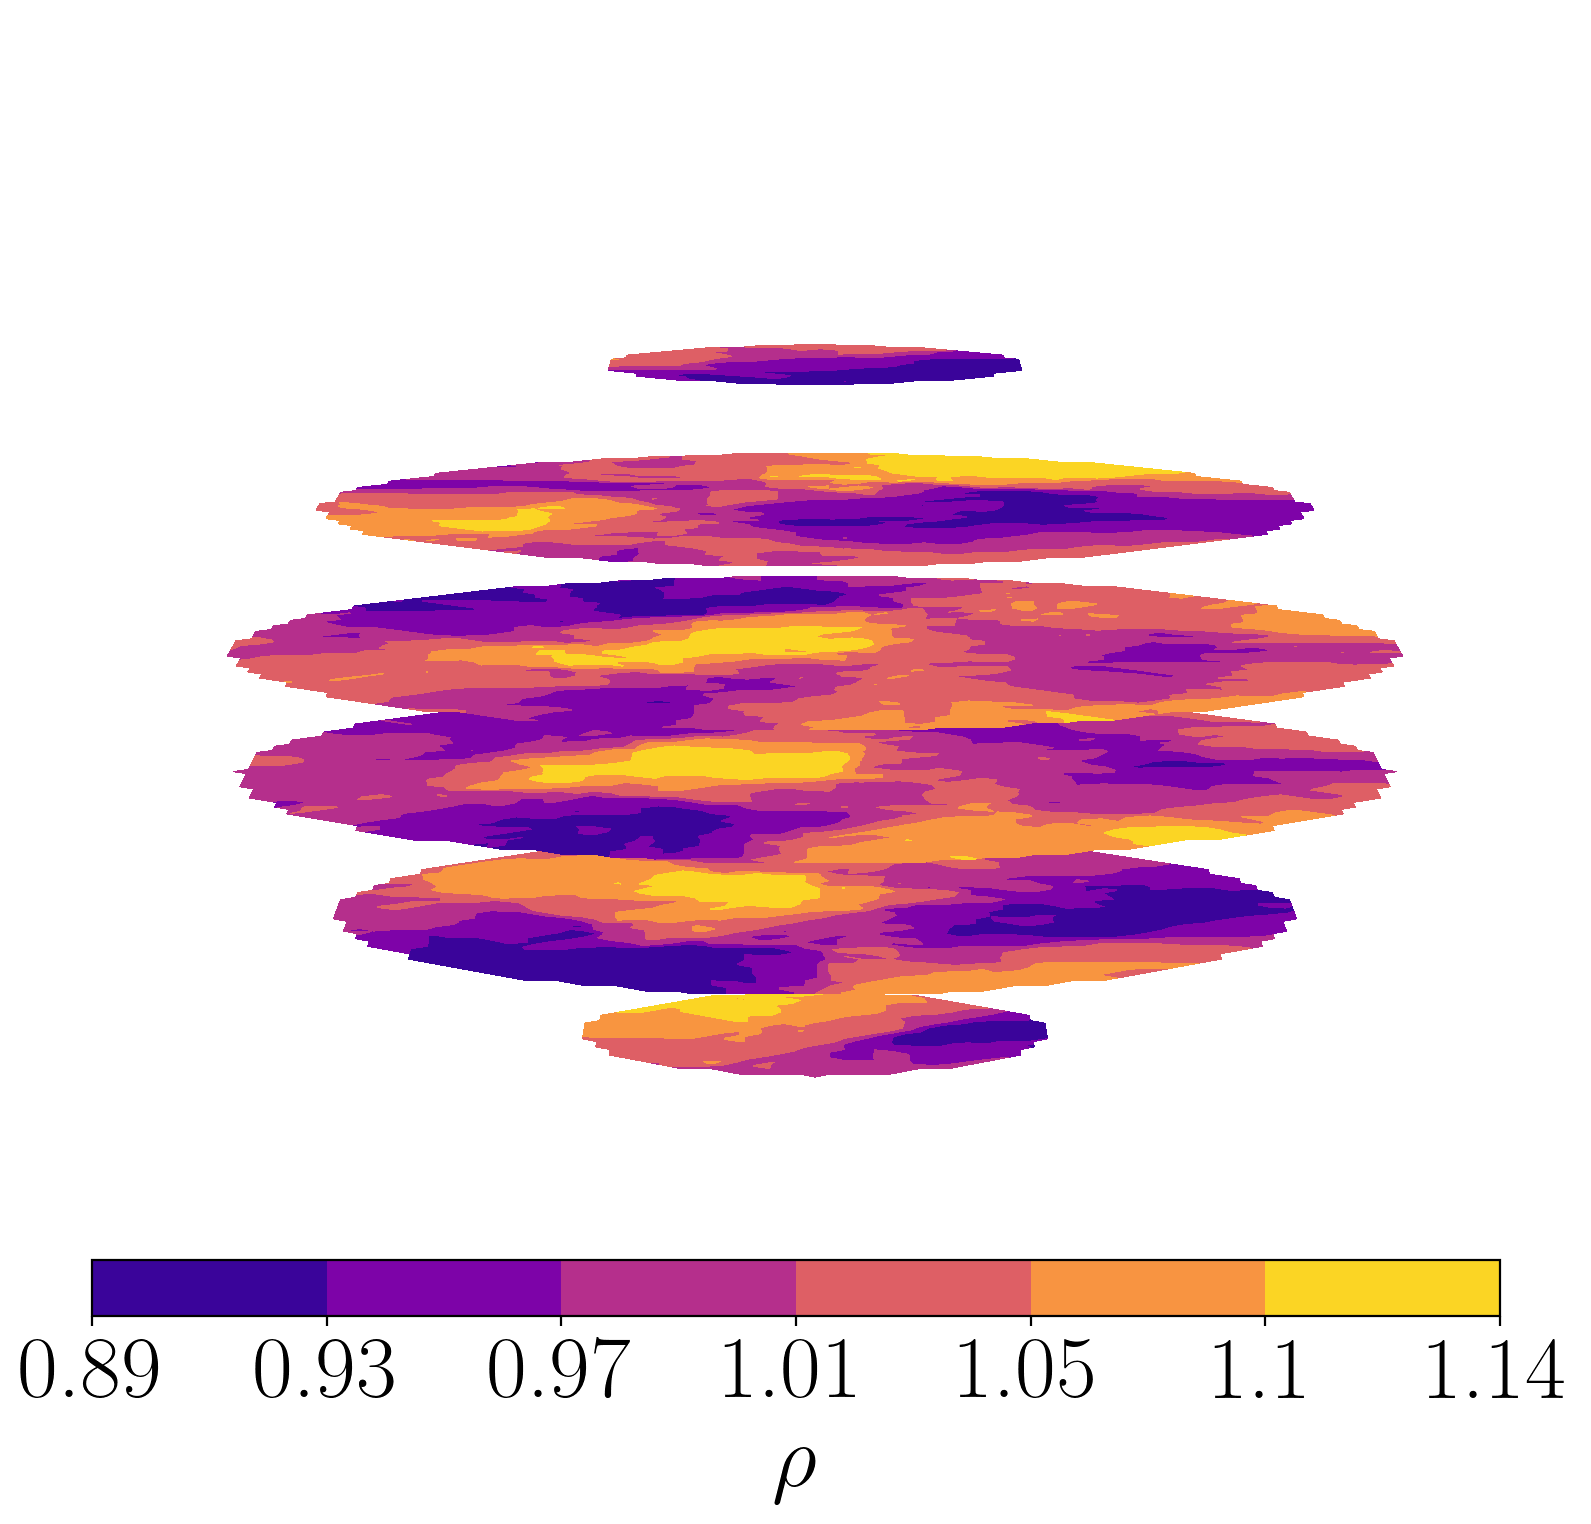
\includegraphics[width=0.24\linewidth]{figs/sym-fe-d}\hfill
  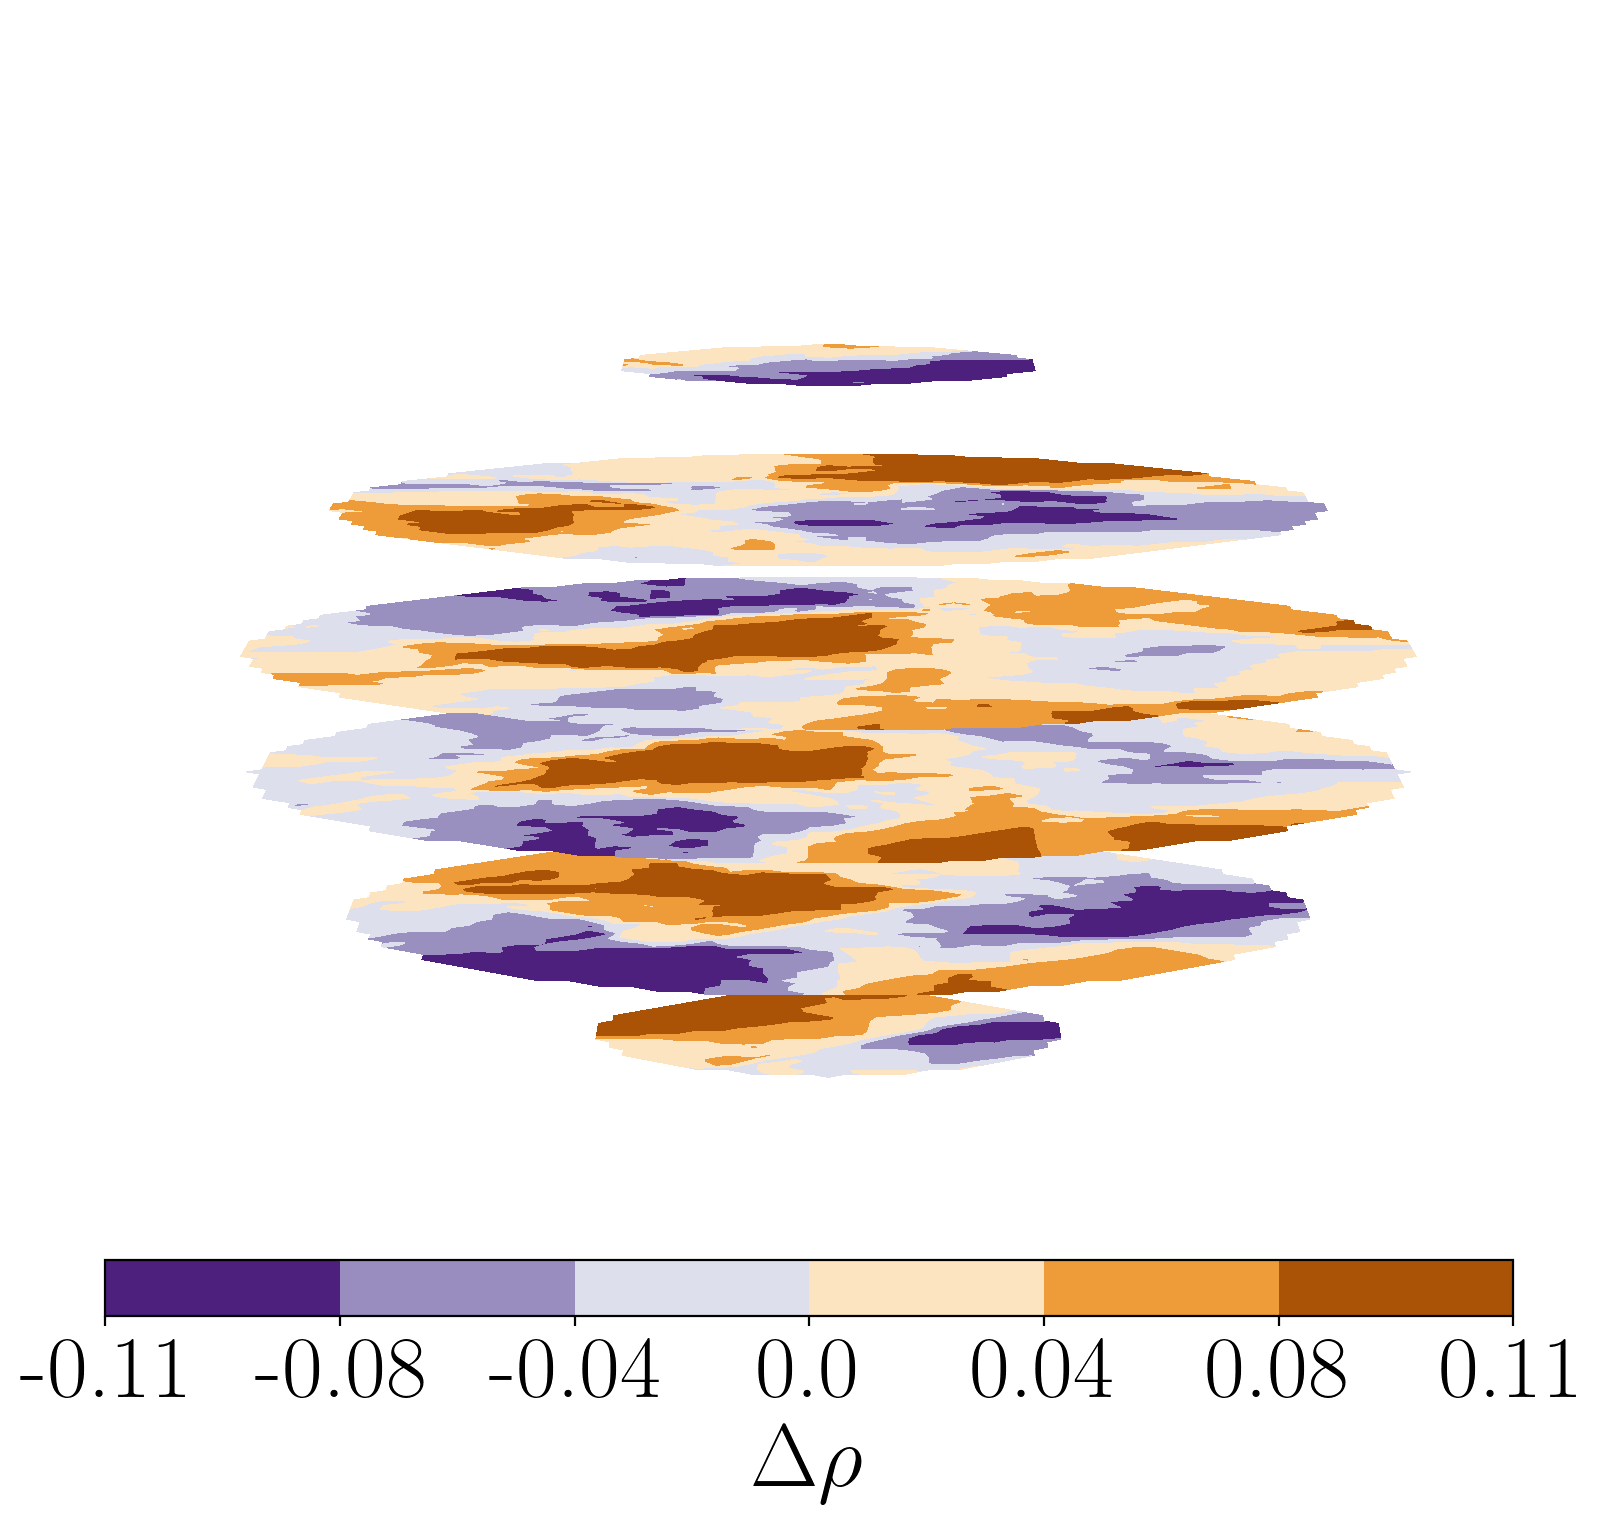
\includegraphics[width=0.24\linewidth]{figs/sym-fe-s}\hfill
  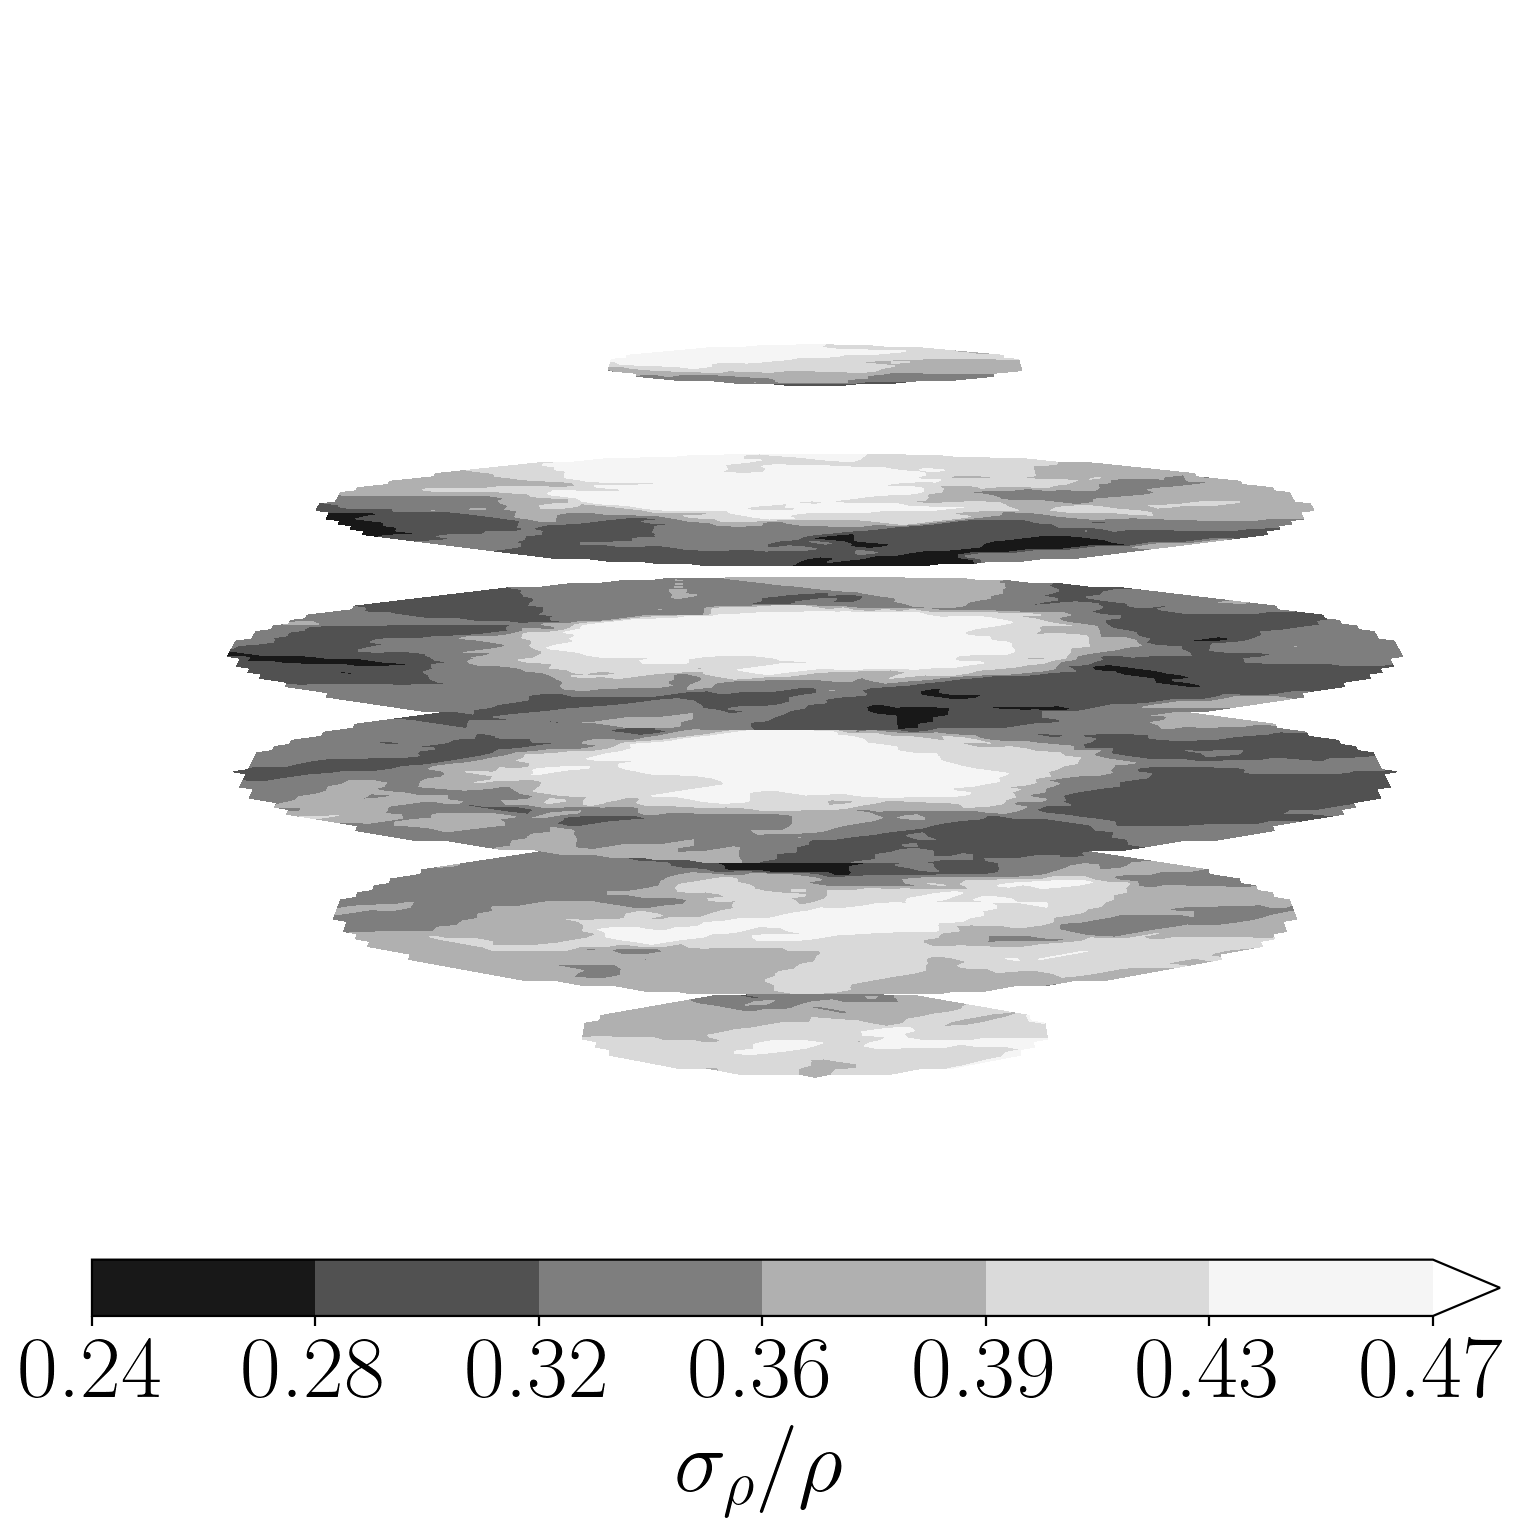
\includegraphics[width=0.24\linewidth]{figs/sym-fe-u}\hfill
  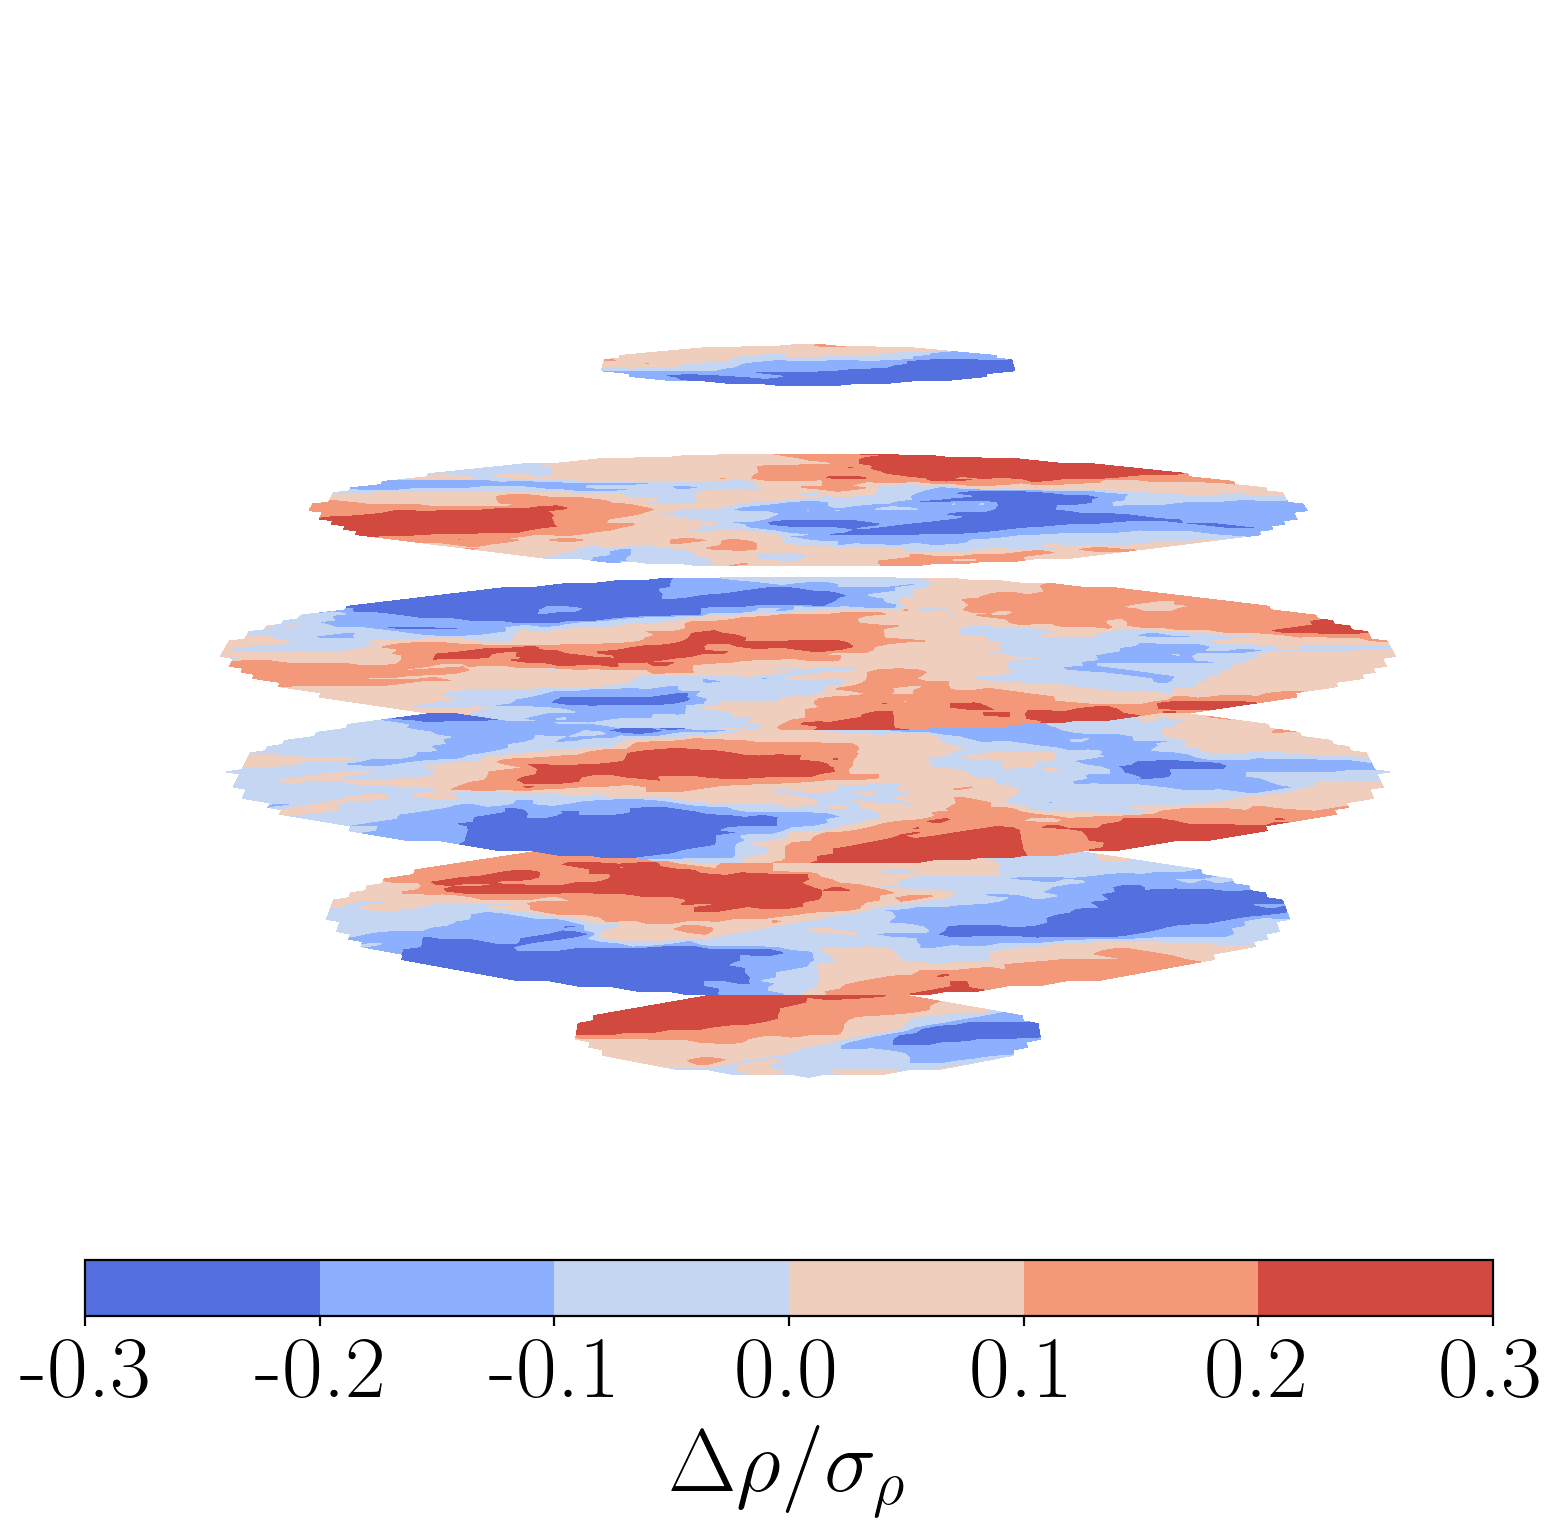
\includegraphics[width=0.24\linewidth]{figs/sym-fe-r}

  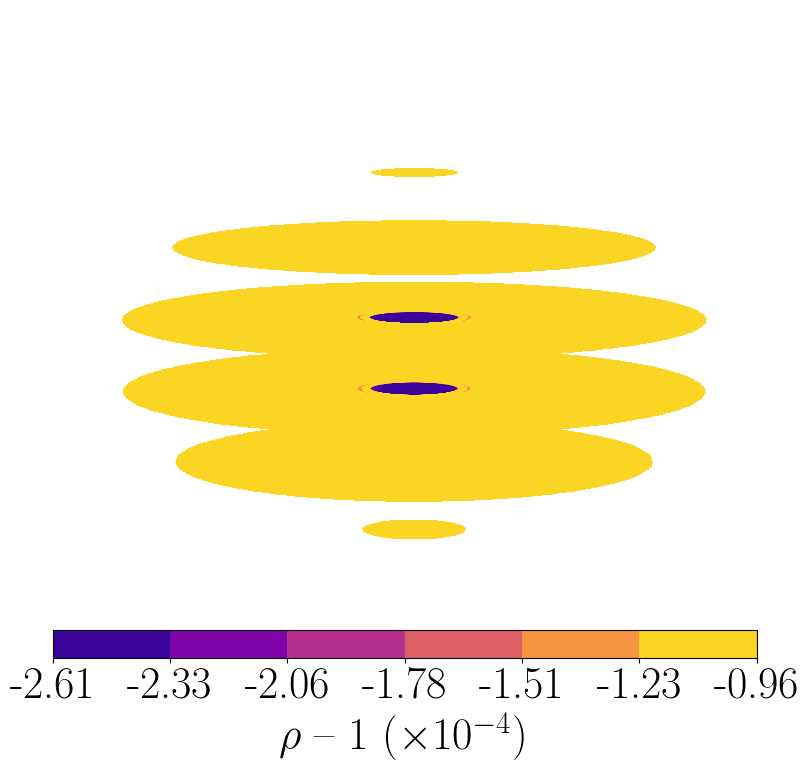
\includegraphics[width=0.24\linewidth]{figs/sym-l-d}\hfill
  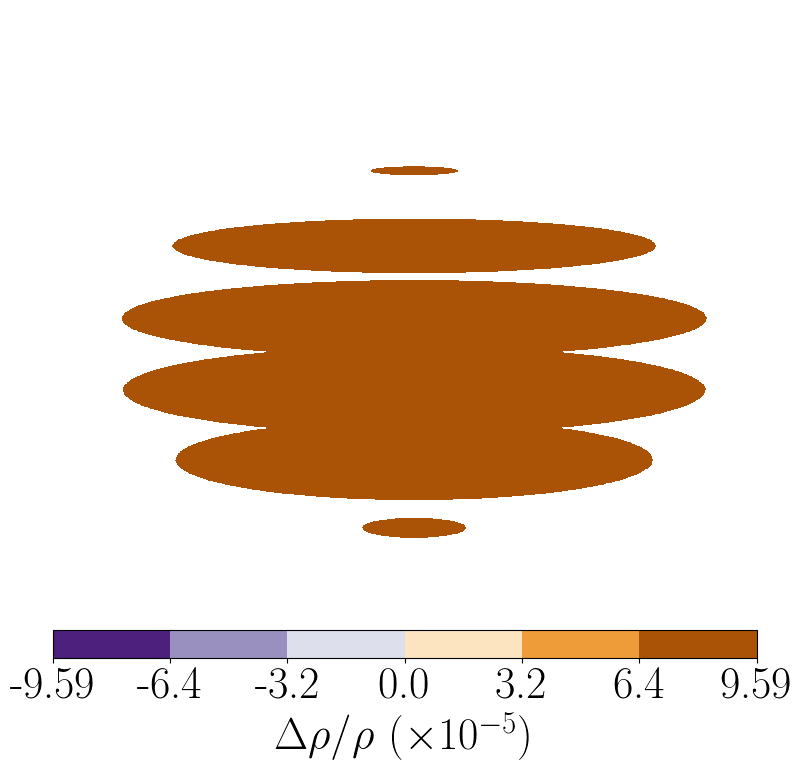
\includegraphics[width=0.24\linewidth]{figs/sym-l-s}\hfill
  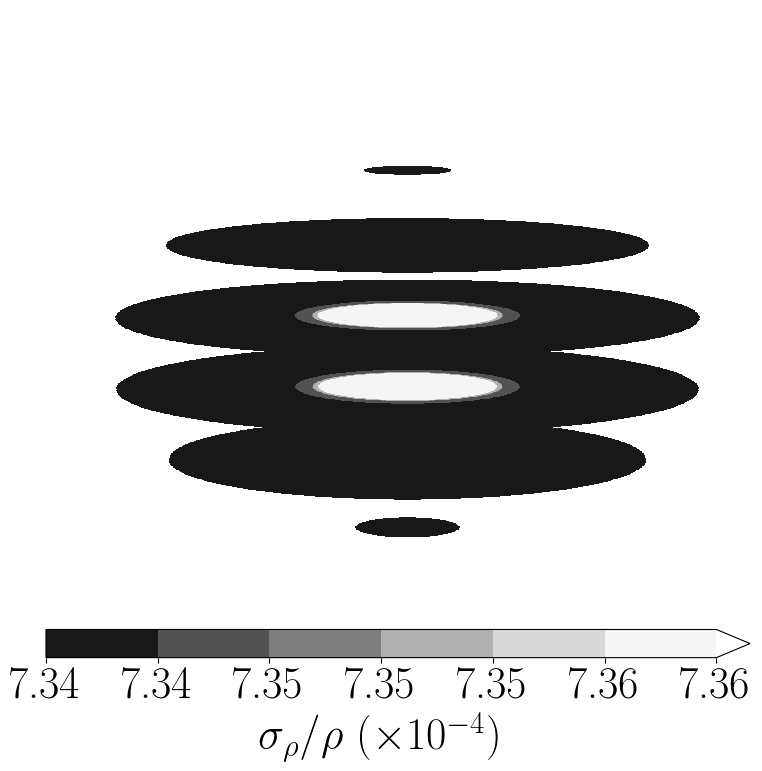
\includegraphics[width=0.24\linewidth]{figs/sym-l-u}\hfill
  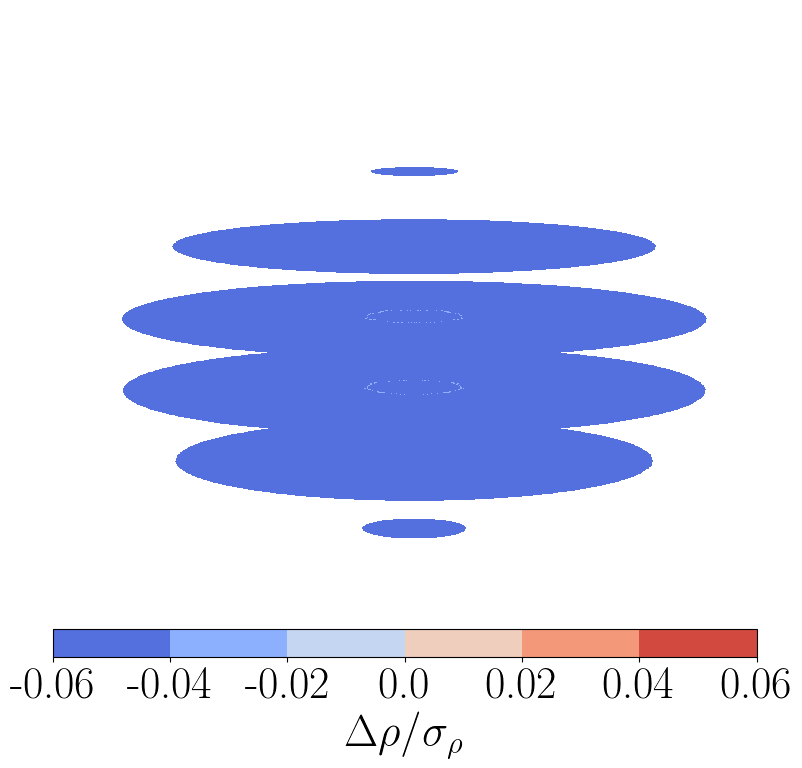
\includegraphics[width=0.24\linewidth]{figs/sym-l-r}

  \caption{Cross-sectional slices of the density distributions extracted via the finite element model for the asymmetric (\textit{first and thrid row}) and symmetric (\textit{second and fourth rows}) reference asteroids. The finite element model (\textit{top two rows}) and the lumpy model (\textit{bottom two rows}) are employed. From left to right, the densities, deviations from the true density, uncertainties, and significance of the deviations are plotted. Extracted densities are generally within 10\% of the truth.}
  \label{fig:uniform}
\end{figure*}

The figure demonstrates that the finite element model successfully extracts density distributions consistent with the extracted density moments, as shown by the $\chi^2$ value per degree of freedom, $\chi^2_r$, depicted in the figure. These express the agreement of the density moments of the shown distributions with the posterior distributions for the density moments, produced by the MCMC described in section \ref{sec:fit}. $\chi^2_r = 0$ indicates that the moments of the shown distributions are exactly equal to the means of the moment posterior extracted by the MCMC. The accuracy of this model is robust for additional shapes, including non-ellipsoidal shapes.

Furthermore, the finite element density distributions are consistent with uniform, which is the true density distribution of the asteroid. For the reference asteroid observational set-up, the uncertainty on observations is such that the density distribution is generally within 10\% of the true density (second column) while the density uncertainty is generally less than 40-50\% of the density value at any point in the asteroid (third column). The dependence of this constraint on the observational set-up is discussed in section \ref{sec:fit-uncertainty}. In no place is the significance of these deviations from the true distribution greater than $0.3 \sigma$ (last column).

The lumpy model also yields distributions which are consistent with the extracted moments and consistent with uniform (the $\chi^2_r$ values are large due to numerical error and correspond to deviations in $K_{2m}$ only on the order of \jtd{number}). These distributions have much lower uncertainty than the finite element distributions (maximum uncertainty on the order of \jtd{number}) due to its few degrees of freedom. With only one lump, the location of the known center of mass requires that the lump lie at the centroid of the asteroid center with mass close to zero and unconstrained radius. Hence, the uncertainty of regions far from the asteroid is typically very small, while regions close to the center are more apt to be contained inside a lump. In order for the lumpy model to converge given the unconstrained lump radius, we use the mass-weighted $\mu_i a_i \rightarrow 0$ as a model parameter rather than the lump length $a_i$.

We also explore model behaviour in non-uniform density asteroids. We employ an asteroid of the same shape as the asymmetric asteroid, and in the same flyby scenario, but we place a solid core of radius $\SI{500}{\meter}$ and density three times the surrounding density at the center of the asteroid. This changes the asteroid density moments. New density moments are extracted via the process described in section \ref{sec:fit} and the finite-element and lumpy models are used to extract density distributions shown in figure \ref{fig:center-core}.
\begin{figure*}
  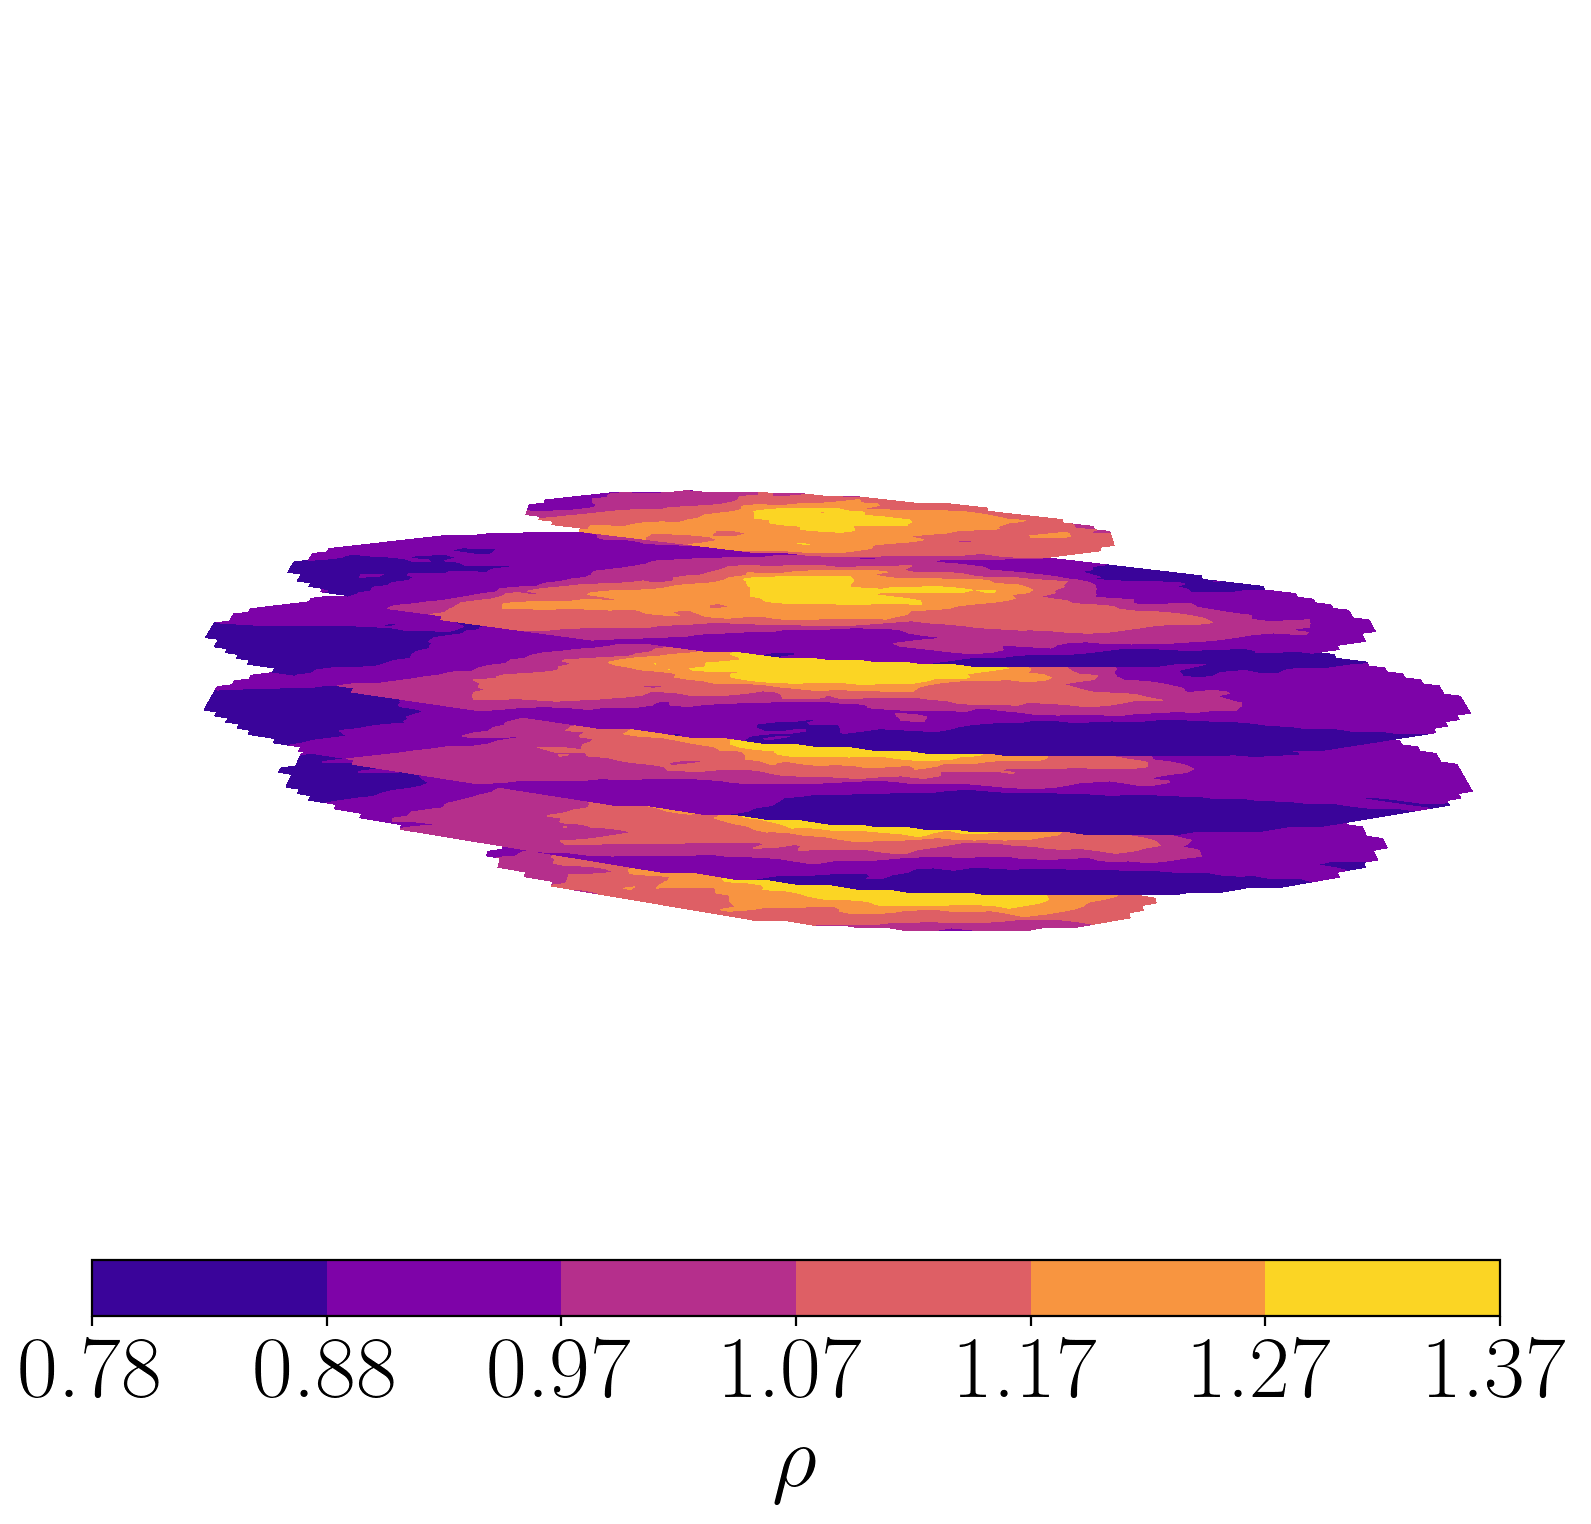
\includegraphics[width=0.24\linewidth]{figs/sph-3-fe-d}\hfill
  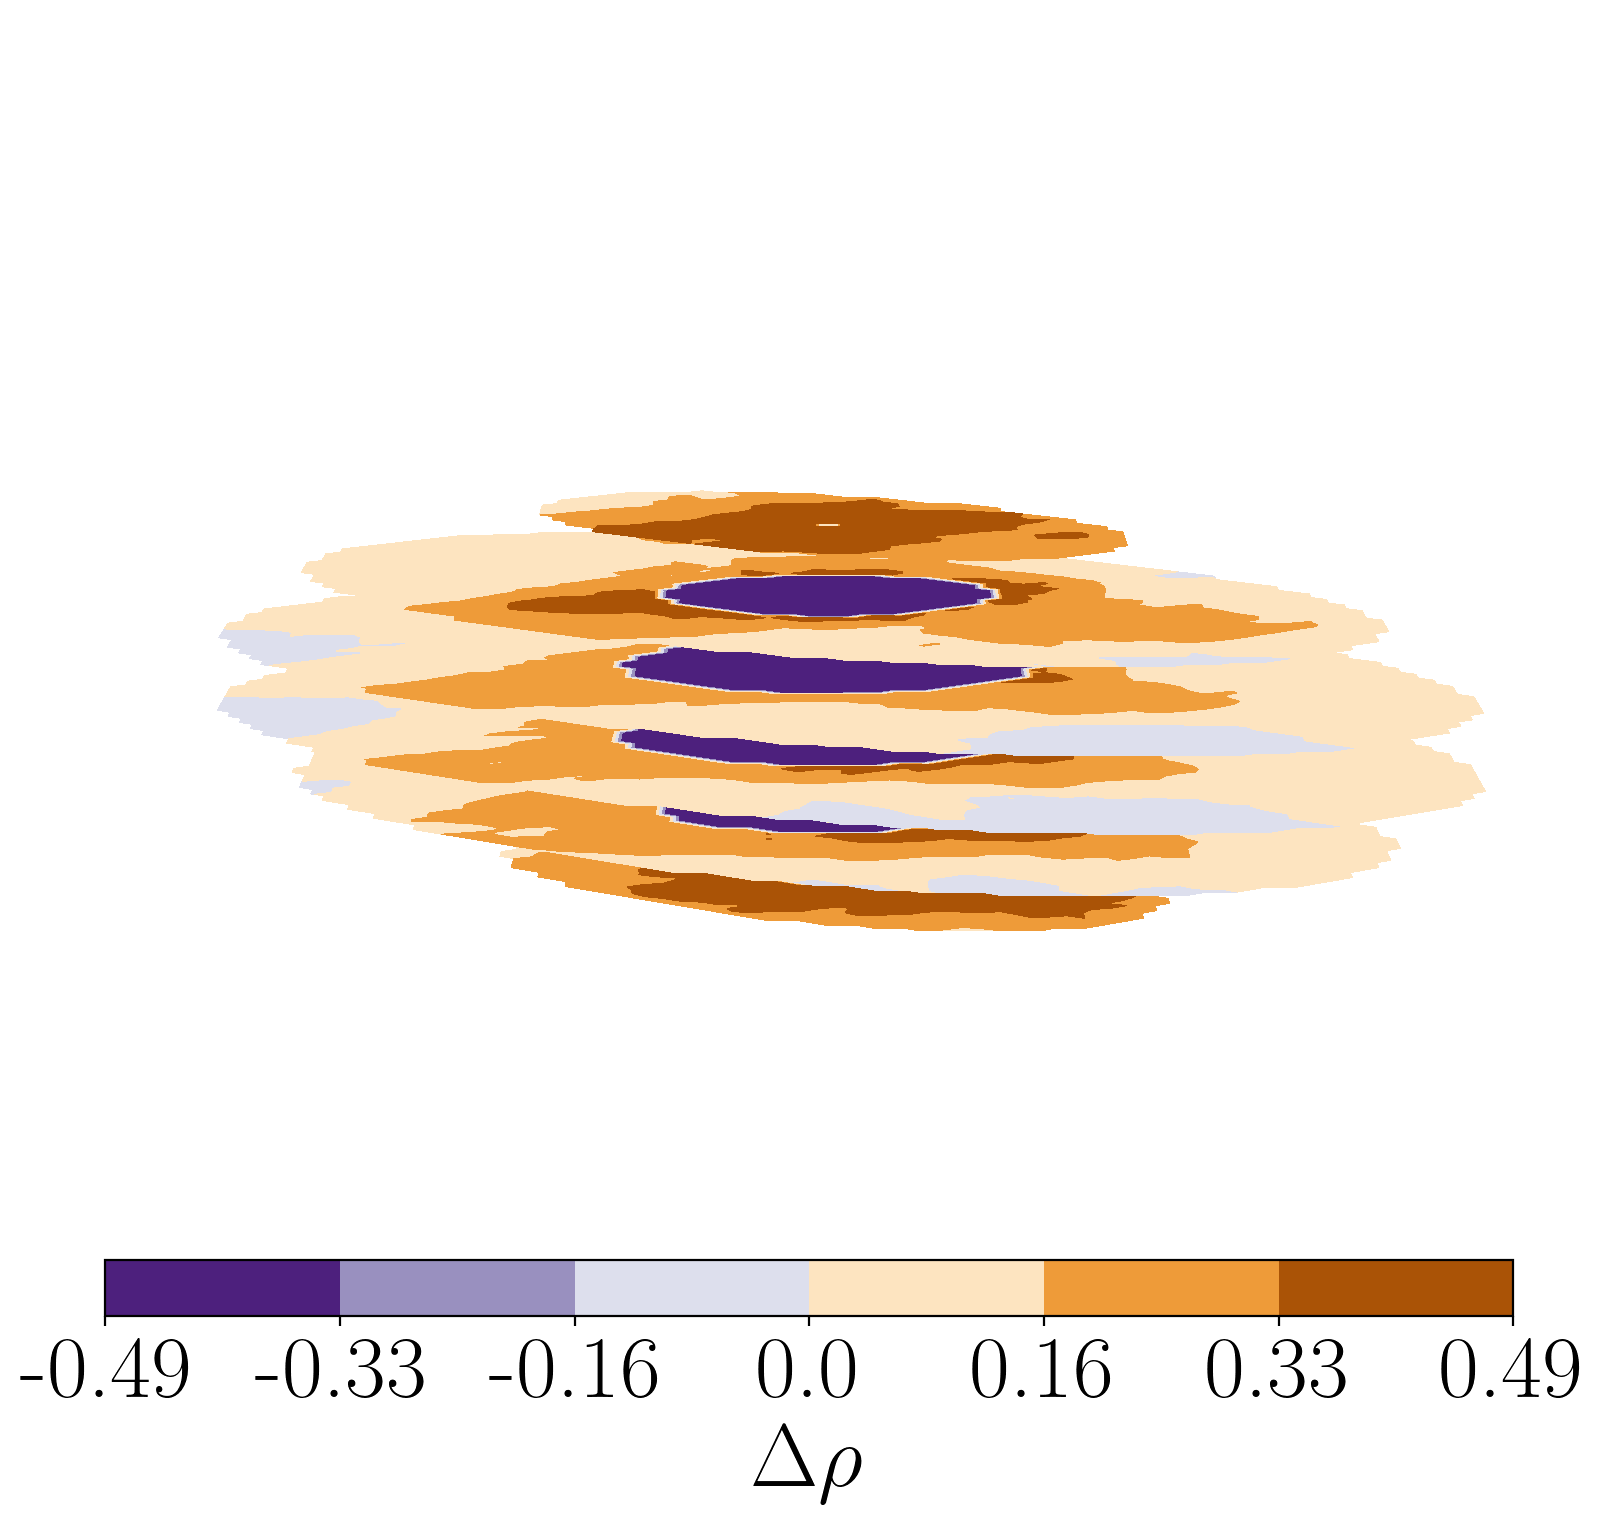
\includegraphics[width=0.24\linewidth]{figs/sph-3-fe-s}\hfill
  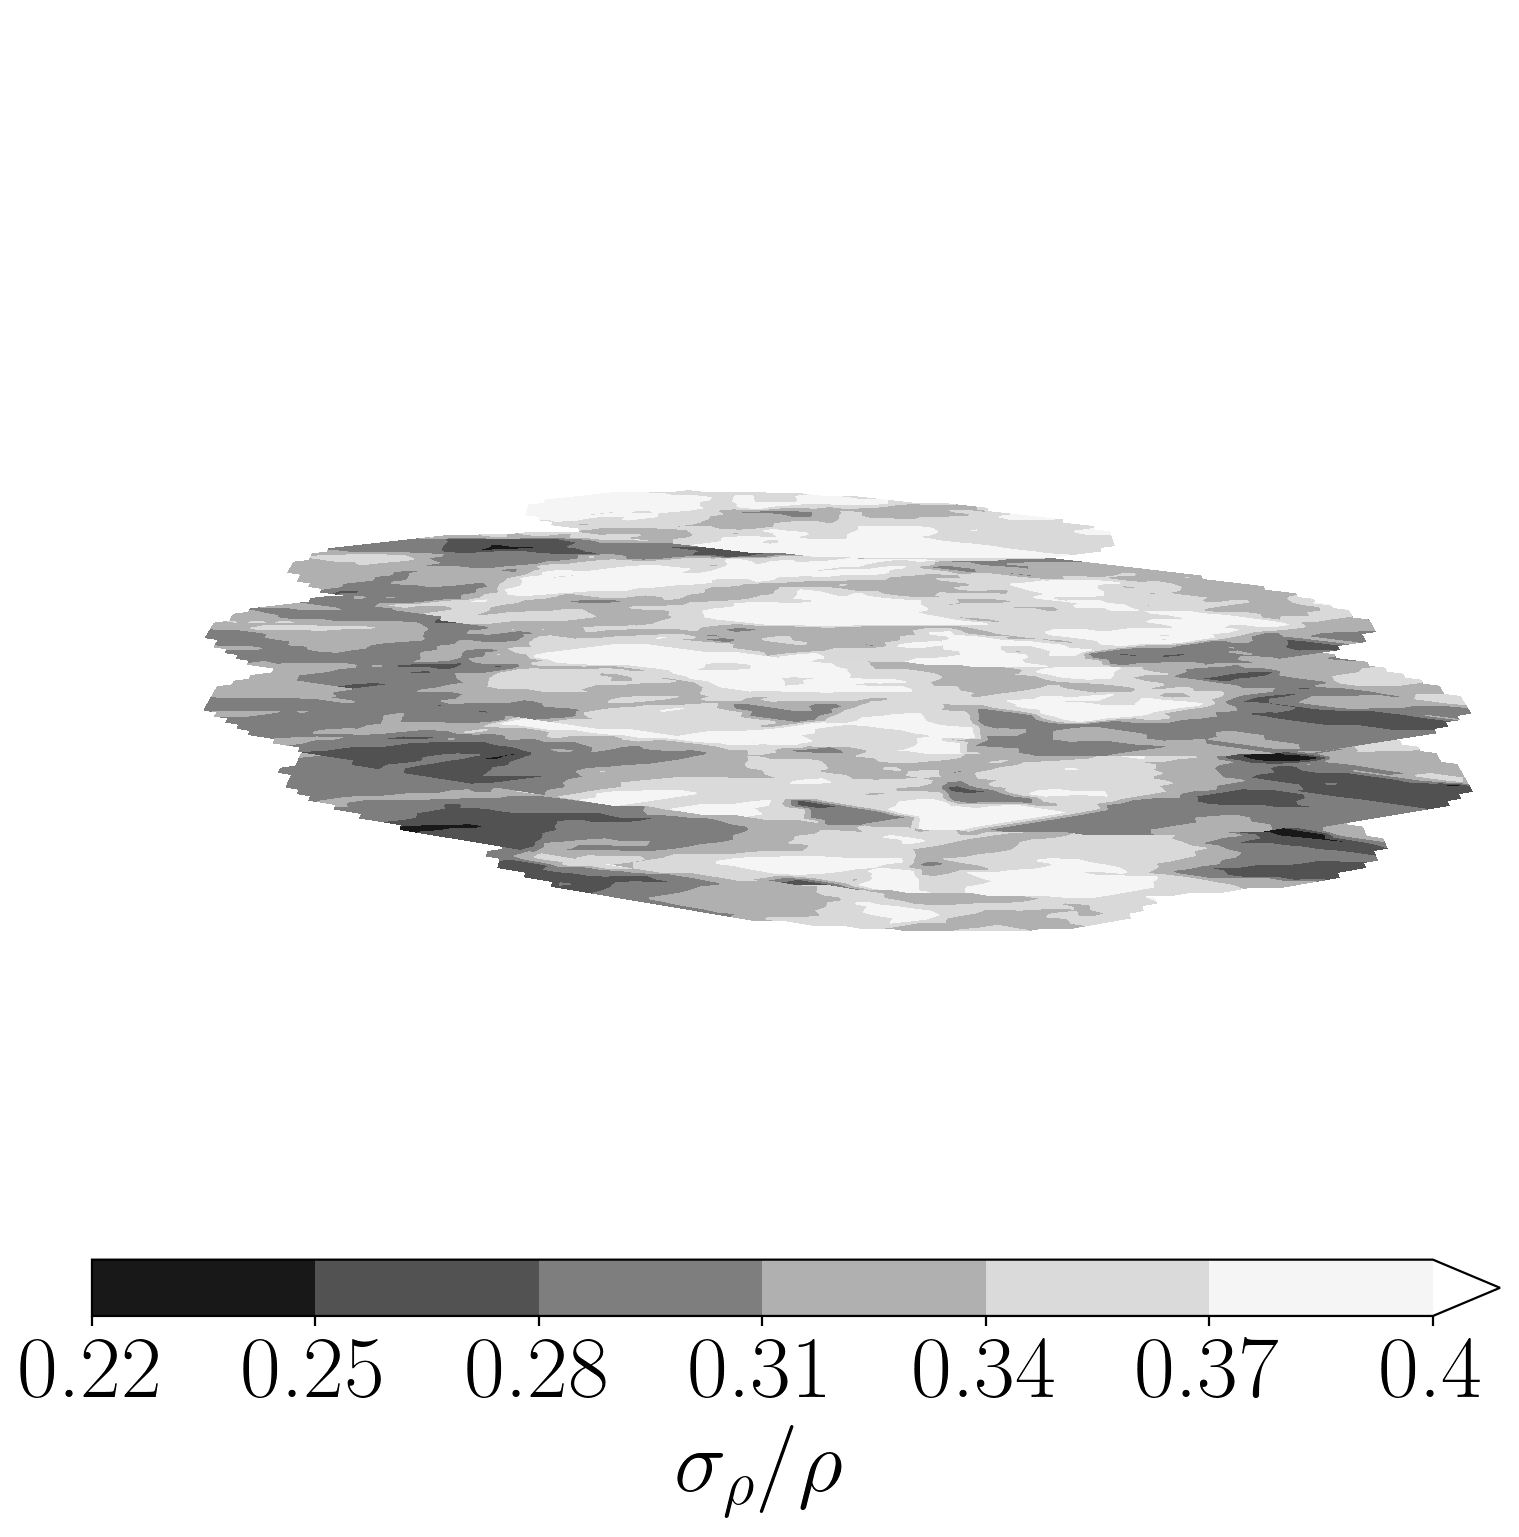
\includegraphics[width=0.24\linewidth]{figs/sph-3-fe-u}\hfill
  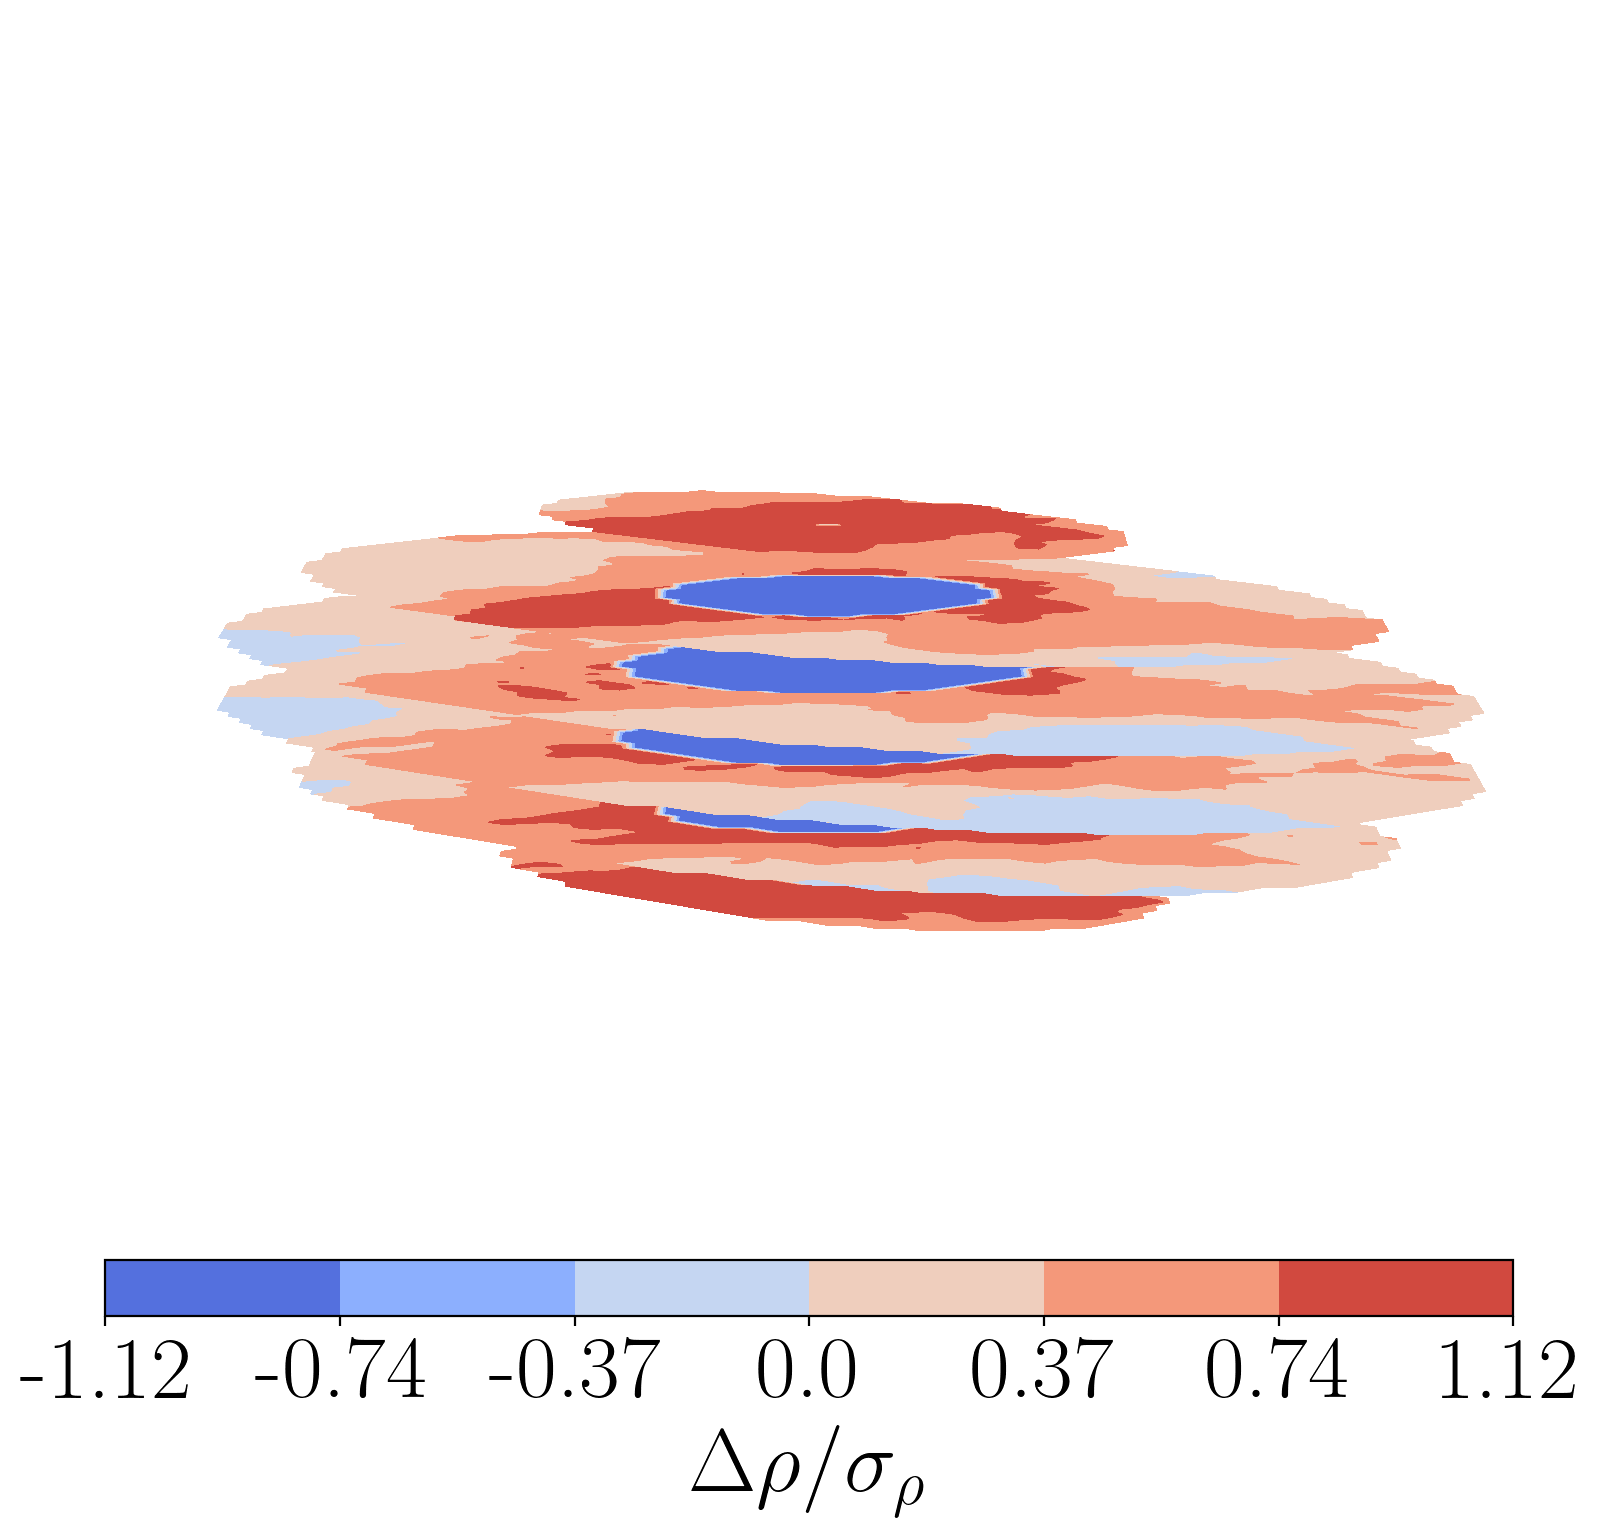
\includegraphics[width=0.24\linewidth]{figs/sph-3-fe-r}

  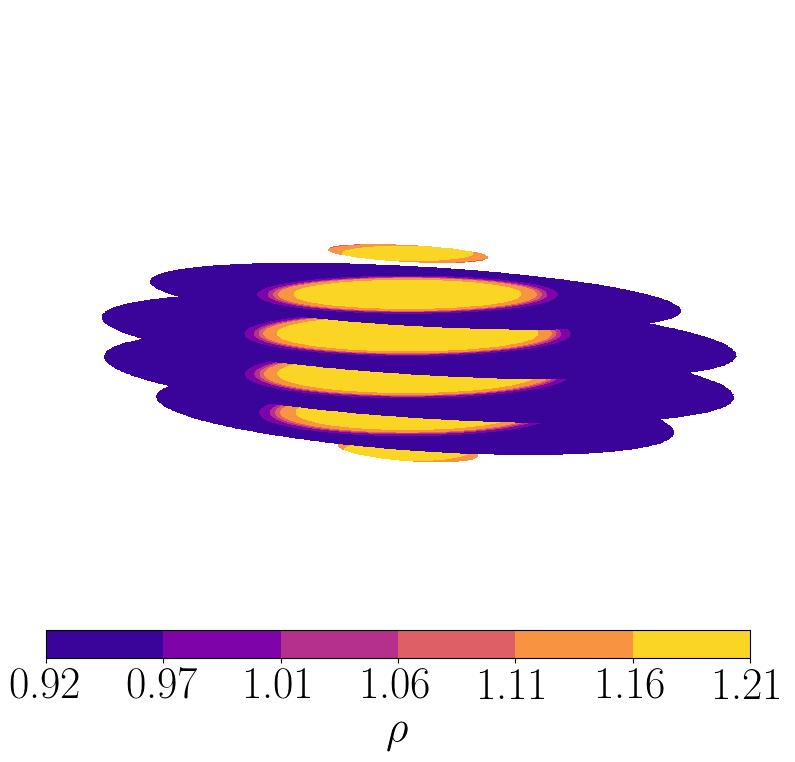
\includegraphics[width=0.24\linewidth]{figs/sph-3-l-d}\hfill
  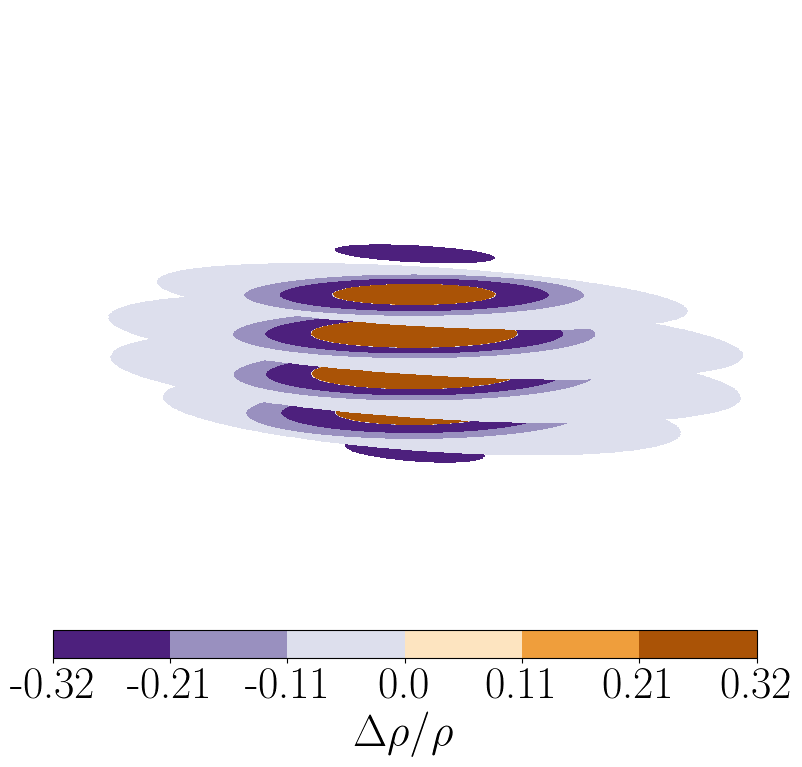
\includegraphics[width=0.24\linewidth]{figs/sph-3-l-s}\hfill
  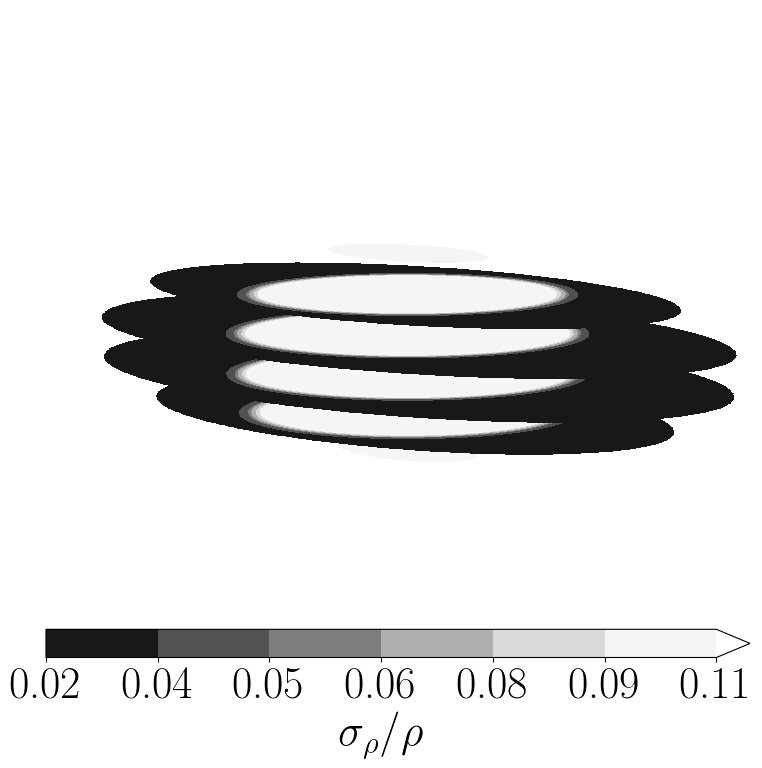
\includegraphics[width=0.24\linewidth]{figs/sph-3-l-u}\hfill
  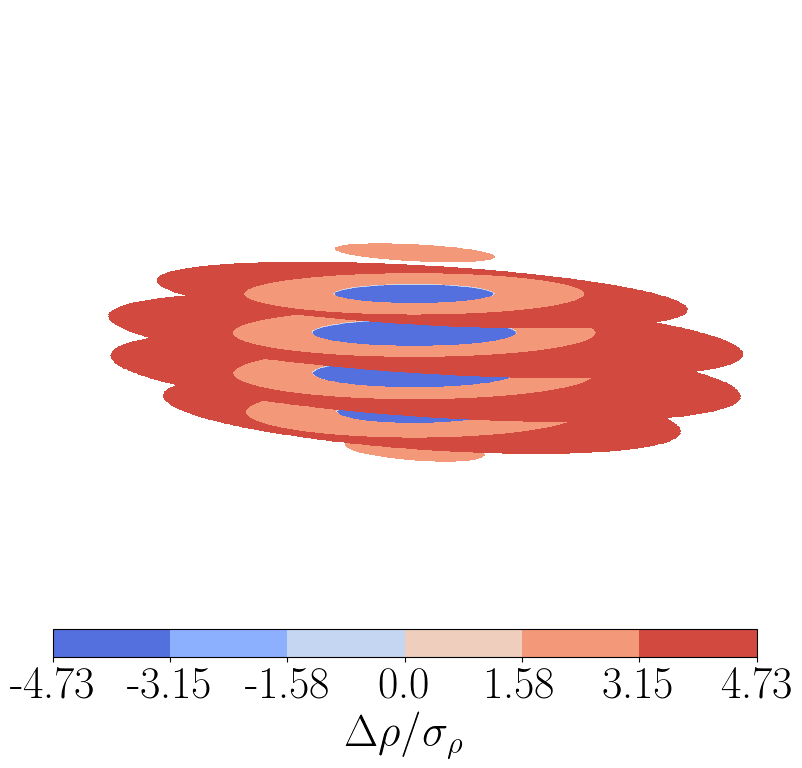
\includegraphics[width=0.24\linewidth]{figs/sph-3-l-r}

  \caption{Cross-sectional slices of the density distributions extracted via the finite-element (\textit{top}) and lumpy (\textit{bottom}) models for an asteroid with a centred core. From left to right, the densities, deviations from the true density, uncertainties, and significance of the deviations are plotted. The core is successfully extracted in all cases.}
  \label{fig:center-core}
\end{figure*}

Once again, figure \ref{fig:center-core} shows that the model results are successful in that they reproduce the extracted density moments ($\chi^2_r$ is low). However, the density distributions extracted by the finite model match the true distributions less well. The deviation the true density extends to as much as 35\% in some locations, leading to a maximum significance of $0.86\sigma$. The distributions are consistent with the true distribution, but the finite element model has distributed the core into the rest of the asteroid so that the peak density is lowered.

However, the lumpy model is designed to detect discrete changes in density distribution, and identifies the boundary of the core very accurately. Deviations from the truth are less than 0.2\%, with uncertainties about 10\% of the local density at maximum and usually much lower. THe significance of the deviations is around 20\%, as it was in figure \ref{fig:uniform} where the extracted distribution again matched the truth. The low uncertainty is caused by the small number of degrees of freedom (2) of the lumpy model. A consequence is that if the core had been non-spherical, the lumpy model would be inaccurate, with significant deviations from the truth. Therefore, neither model is more correct in the general case, but each can be used to explore different scenarios.




\section{Discussion}
\label{sec:discussion}

% In this section, we discuss the sensitivity of our results to the properties of the asteroid encounter system. We start with the encounter properties that are required to adequately constrain the asteroid's density moments and distribution, and further discuss the properties of Jupiter encounters compared to Earth encounters. Finally, we discuss in greater detail which features of an asteroid density distribution can be extracted by our models and which cannot be.

\subsection{Dependence of uncertainty on encounter properties}
\label{sec:fit-uncertainty}


The question of which encounters are most suited to this analysis is of great interest. We investigate a mix of encounter parameters, from observational parameters (e.g., the cadence of observations, gaps in data, and uncertainty in the spin pole and period of the asteroid) and physical asteroid properties (e.g., the true density moments, rotational period, perigee, excess velocity, initial spin pole direction, and length), and discuss their effect on the uncertainty of this methodology's results.

Specifically, we highlight both the uncertainties on the density moments and uncertainty on density distribution. Moment uncertainty is defined as the range of $K_{\ell m}$ values that contains 68.27\% of the marginal PPD for each $\ell$ and $m$. Since there is no degeneracy between moments and the actual encounter data, this uncertainty is well-defined. However, its physical relevance is not obvious. The density distribution uncertainty is presented as a map of uncertainty over the asteroid, made by taking the standard deviation of density at each point over 5000 maps of asteroid density, each made using a different sample of the output of the density distribution MCMC described in section \ref{sec:density-distro}. The average uncertainty over this map, divided by the local density, is taken as the uncertainty in density distribution of the asteroid. This measure of uncertainty is more physically relevant than moment uncertainty, but it is affected by choices of the density distribution model, degrees of freedom, prior constraints, and other effects unrelated to the encounter properties.

We therefore investigate both the moment uncertainty and the density distribution uncertainty. Figure \ref{fig:scan-physical} displays the dependence of moment uncertainty on four asteroid physical parameters and and \ref{fig:scan-observational} displays dependence on observational parameters. Additionally, figures \ref{fig:scan-space-sigma} and \ref{fig:scan-spin} display dependence on asteroid shape and initial spin direction. These are useful as a sensitive and model-independent measure of the relationship between the encounter properties and the methodology uncertainty.


\begin{table}
  \centering
  \begin{tabular}{lll} \hline
    Encounter property & $\sigma_\rho / \rho = 100\%$ & $20\%$ \\ \hline
    Perigee ($r_p$, Earth radii) & $<$7.9 & $<$4.7 \\
    Excess velocity ($v_\infty$) & - & - \\
    Asteroid length ($a_\mathcal{A}$, m) & $>$180 & $>$1100 \\
    Period ($P_\omega$, hr) & $>$4.3 & $>$9.5\\ \hline
    Spin period uncertainty ($P_\omega \sigma_\rho$, ms) & $<$15 & $<$3.1\\
    Spin pole uncertainty ($\sigma_\theta$, $^\circ$) & $<$2.8 & $<$0.5 \\
    Cadence ($\Delta t$, min) & $<$38 & $<$2 \\
    Data gap ($T_\text{gap}$, hr) & $<$1.8 & $<$0 \\ 
    \hline
  \end{tabular}
  \caption{The physical / observational encounter property thresholds (\textit{top} / \textit{bottom} consistent with useable density distribution uncertainty. \jtd{Summarizing sentence}.}
  \label{tab:threshold-summary}
\end{table}

In table \ref{tab:threshold-summary}, we present the property ``thresholds'' required in order to obtain meaningful information about the asteroid density distribution. These are collected by \jtd{Explain}. Their values are also shown in figures \ref{fig:scan-physical} to \ref{fig:scan-observational} as vertical red lines. These thresholds are more physically relevant, but they should be understood as moveable, since making different model choices can drastically change their locations.

\begin{figure*}
  \newpage
  \centering
  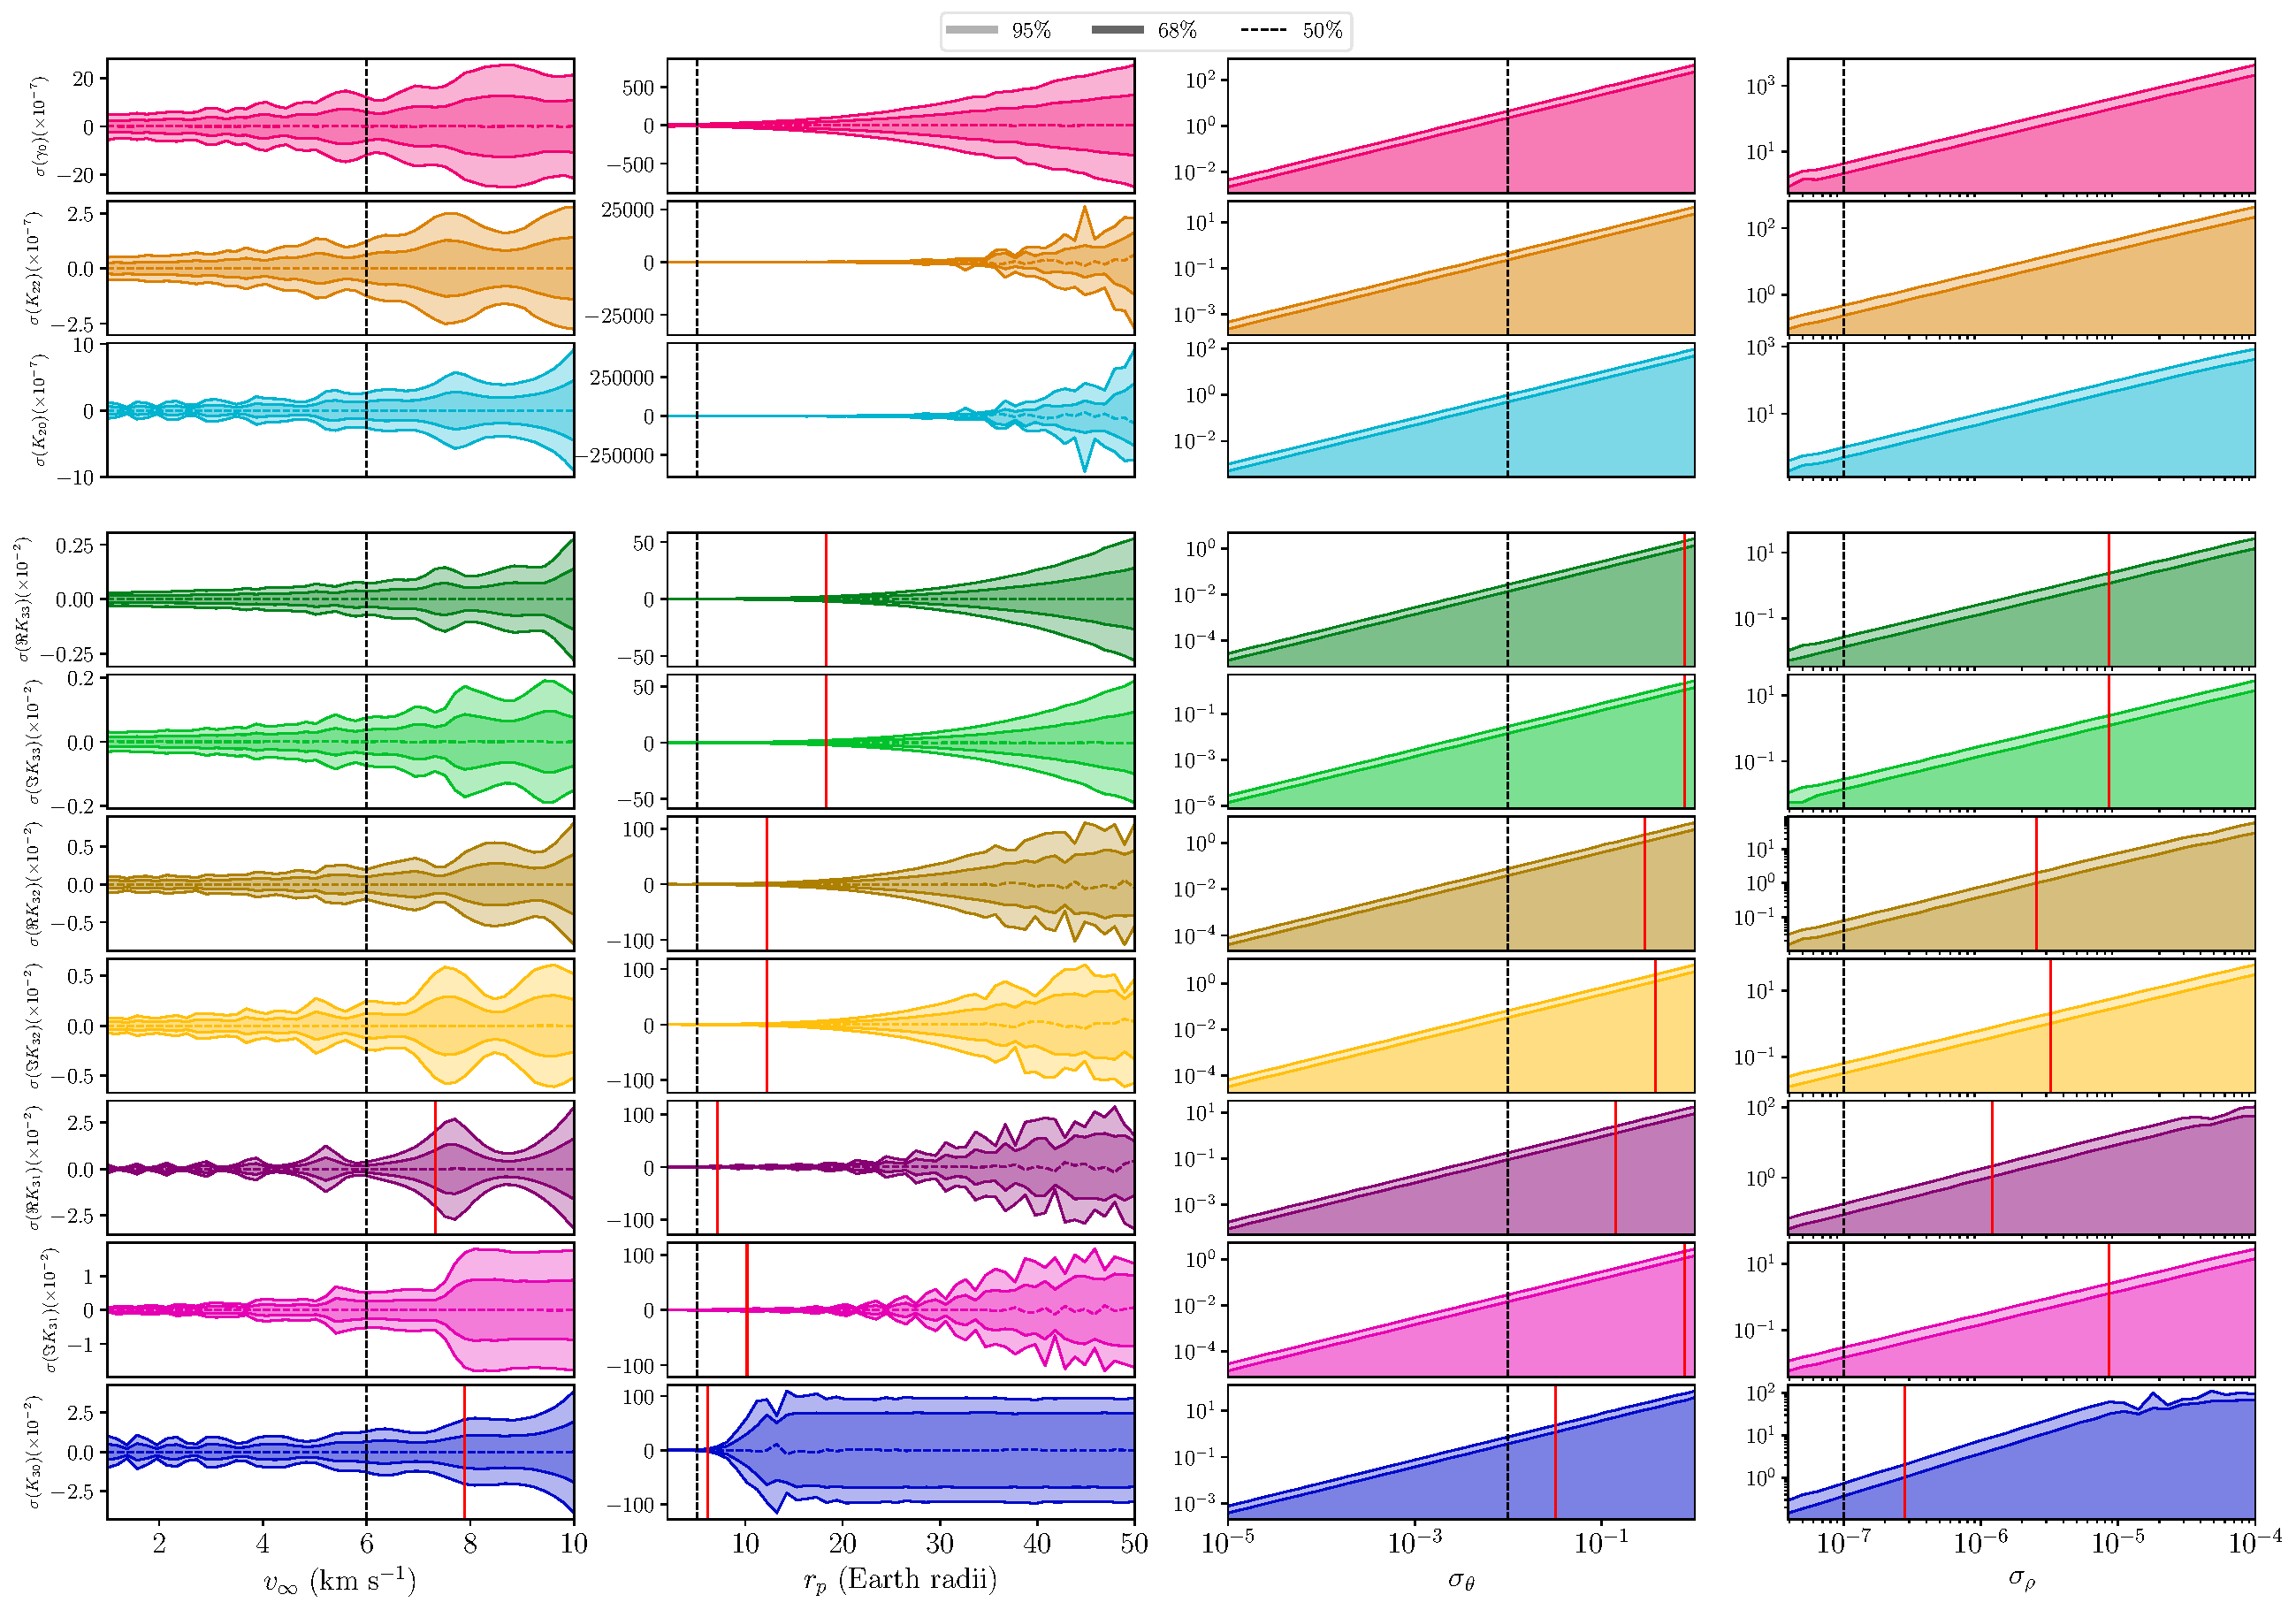
\includegraphics[angle=90, origin=c, width=\linewidth]{figs/scan-all1.pdf}
  \caption{1 and 2$\sigma$ confidence intervals for the first-order parameter PPDs (\textit{top}) and second-order parameters (\textit{bottom}) as a function of (left to right) perigee, excess velocity, spin pole uncertainty, and period uncertainty. The vertical dashed line indicates the reference asteroid values. The red vertical lines indicate when $\sigma(K_{3m}) =0.01$.}
  \label{fig:scan-perigee}
  \label{fig:scan-vex}
  \label{fig:scan-am}
  \label{fig:scan-period}
  \label{fig:scan-physical}
\end{figure*}

\begin{figure*}
  \newpage
  \centering
  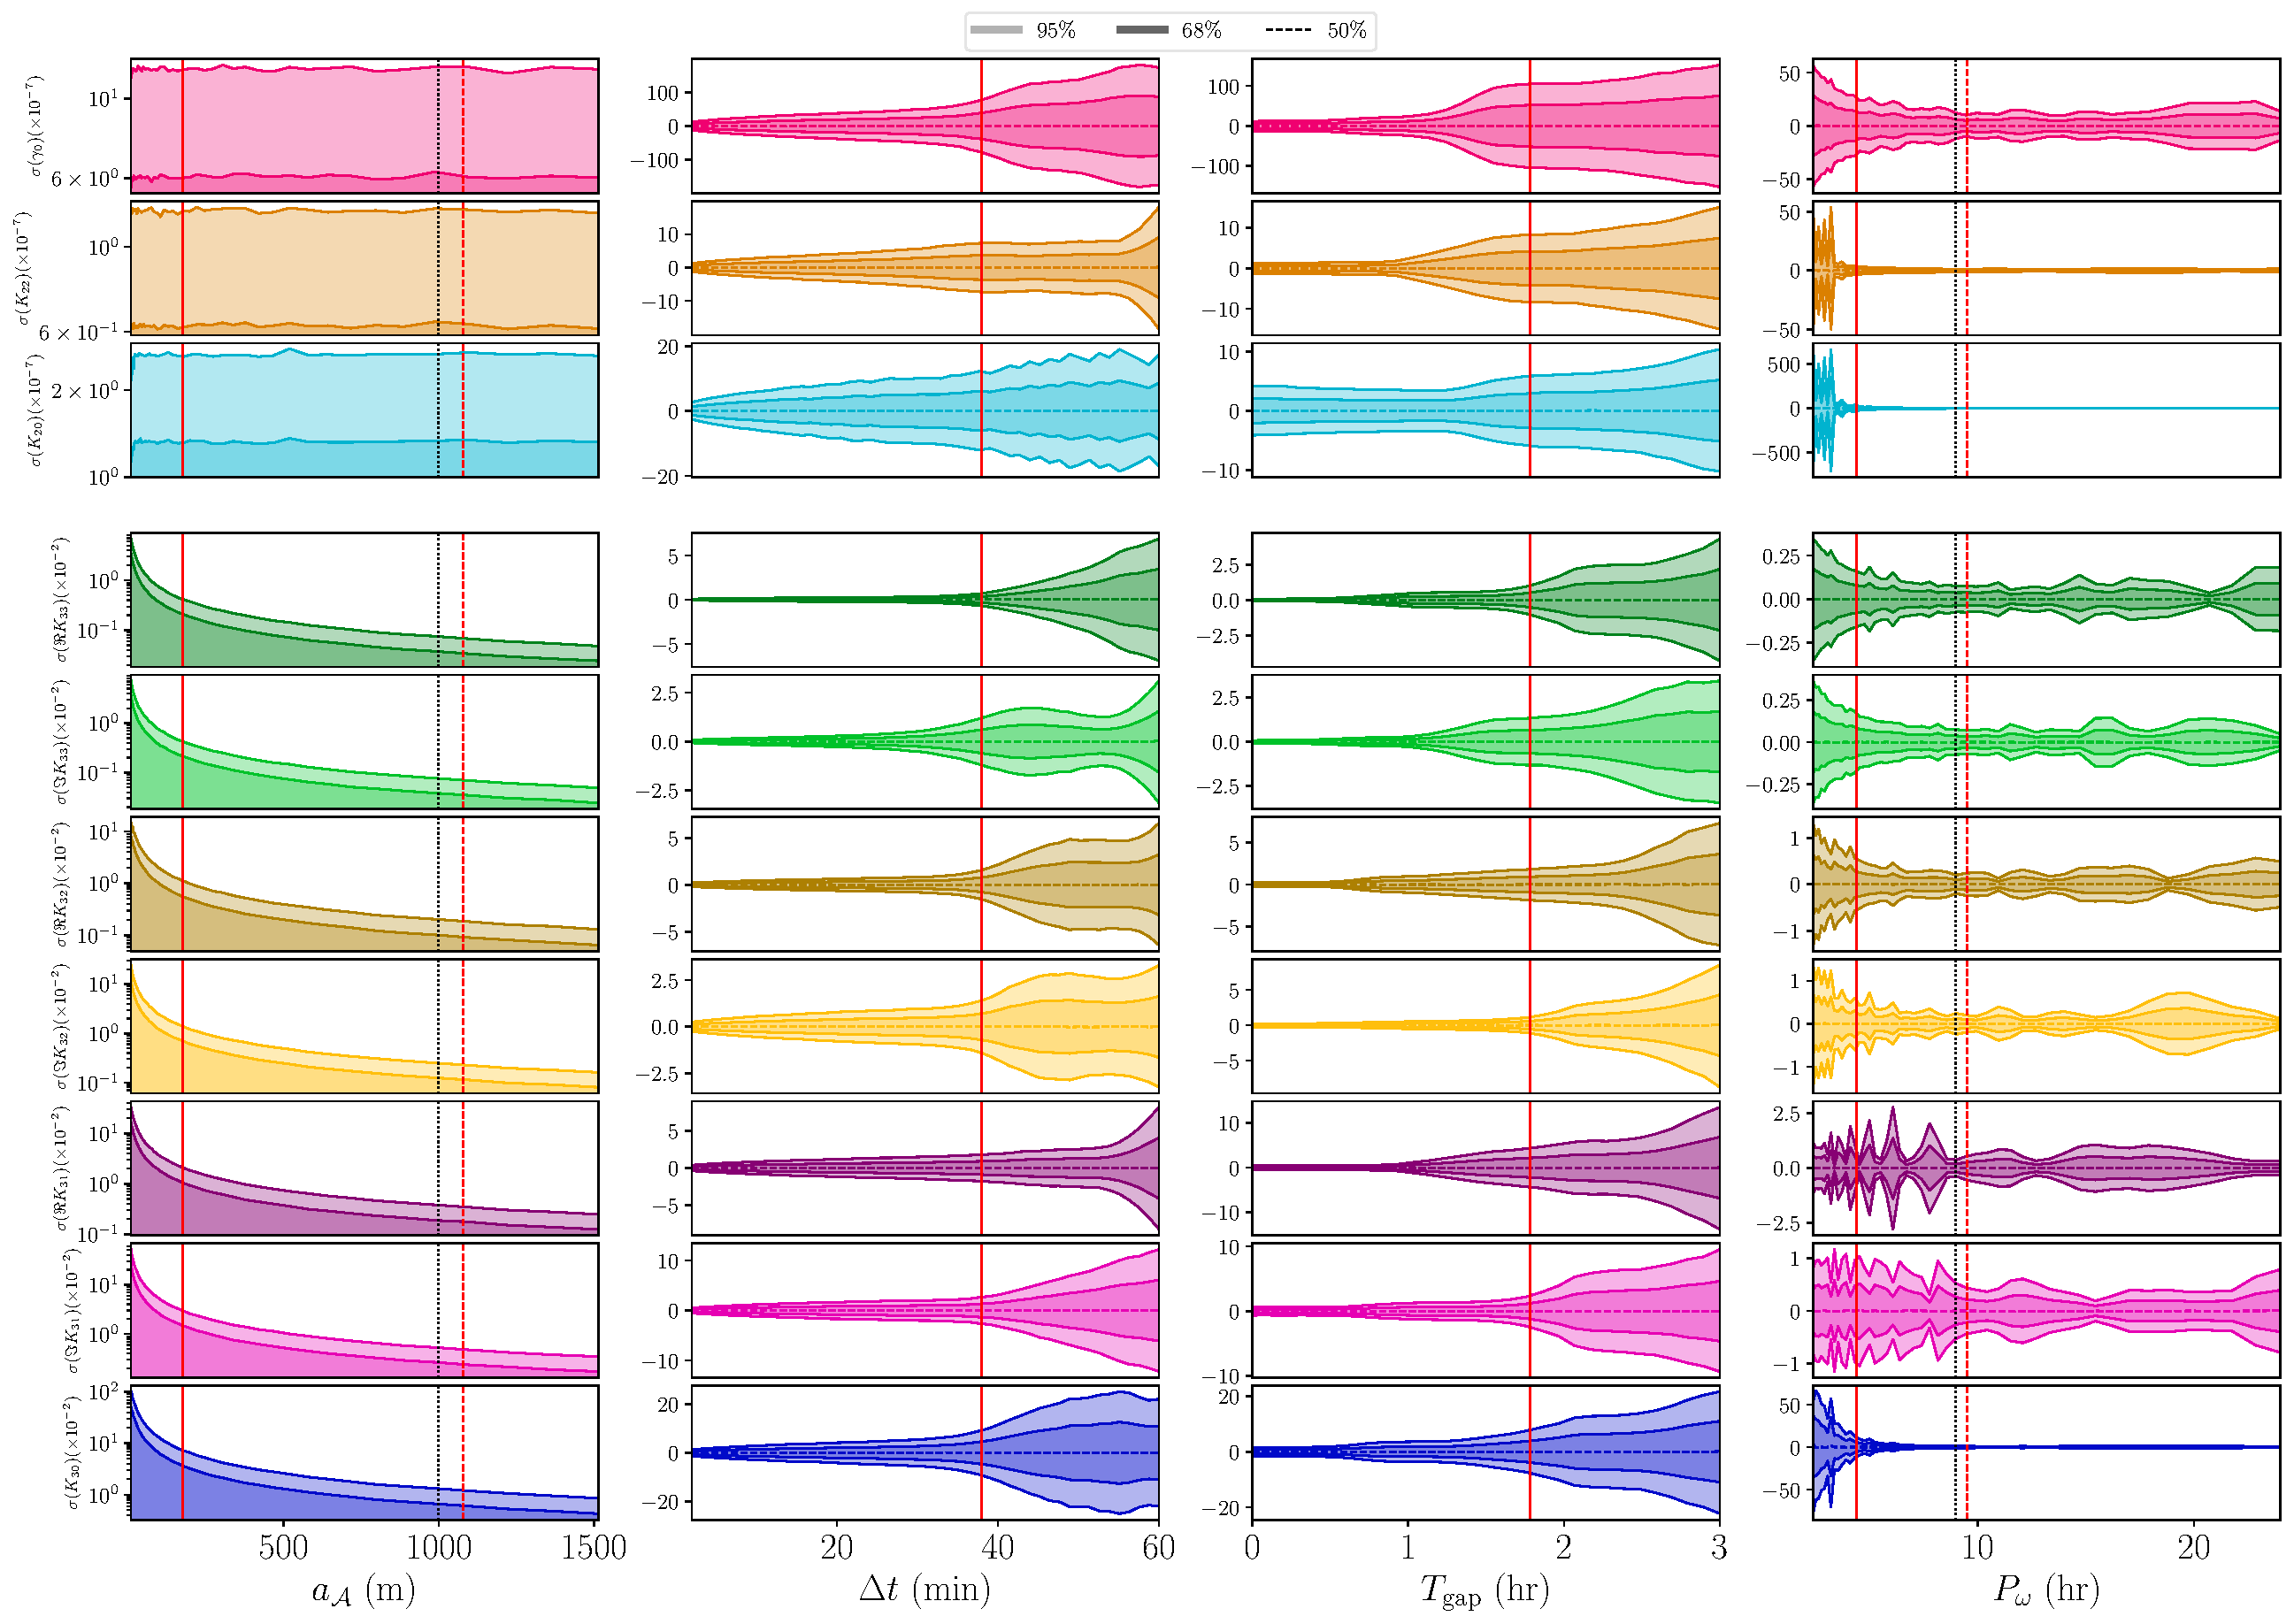
\includegraphics[angle=90, origin=c, width=\linewidth]{figs/scan-all2.pdf}
  \caption{1 and 2$\sigma$ confidence intervals for the first-order parameter PPDs (\textit{top}) and second-order parameters (\textit{bottom}) as a function of (left to right) asteroid length, observational cadence, data gap at perigee, and rotational period. The vertical dashed line indicates the reference asteroid values. The red vertical lines indicate when $\sigma(K_{3m}) =0.01$.}
    \label{fig:scan-rho}
    \label{fig:scan-theta}
    \label{fig:scan-cadence}
    \label{fig:observation-gap}
    \label{fig:scan-observational}
\end{figure*}

\begin{figure*}
  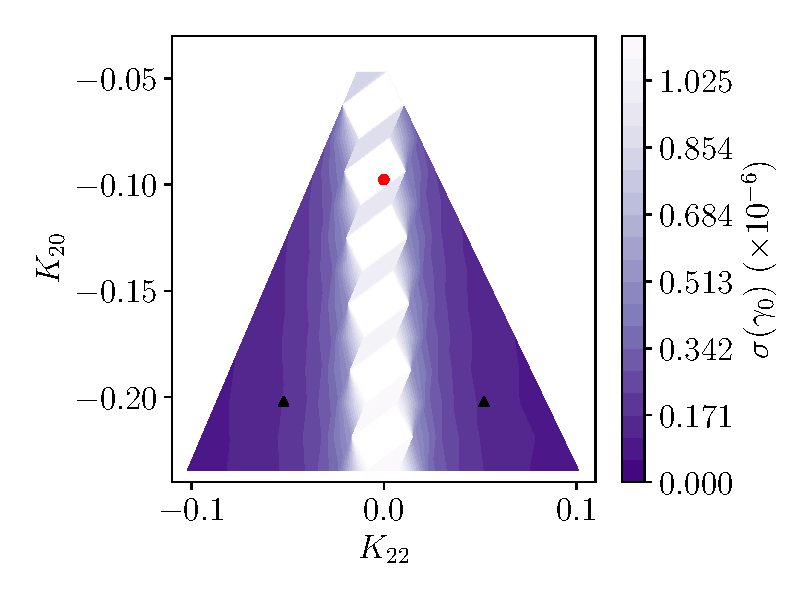
\includegraphics[width=0.3\textwidth]{figs/probe-space-theta-1-sigma.pdf}\hfill
  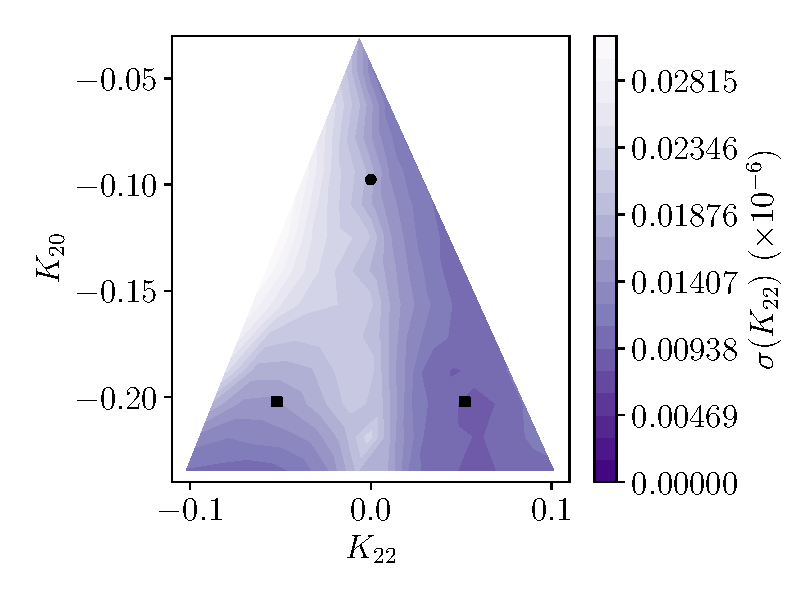
\includegraphics[width=0.3\textwidth]{figs/probe-space-theta-2-sigma.pdf}\hfill
  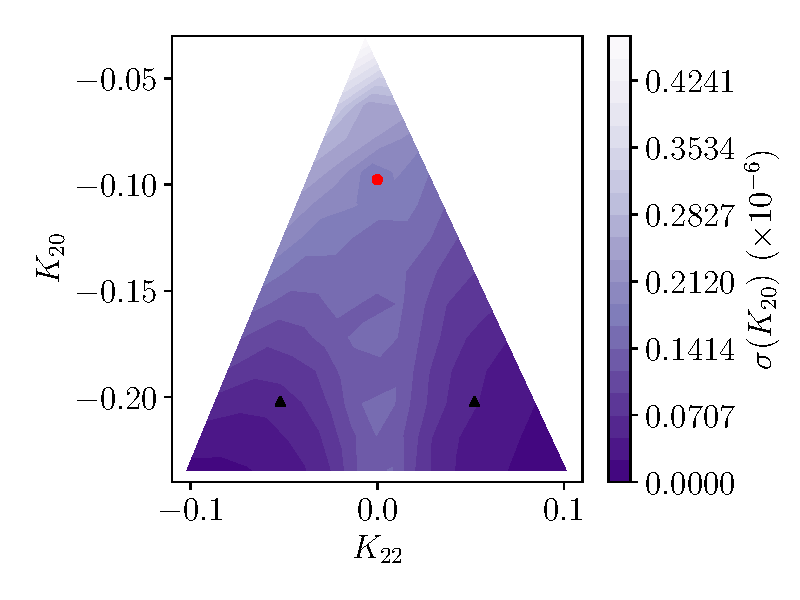
\includegraphics[width=0.3\textwidth]{figs/probe-space-theta-3-sigma.pdf}

  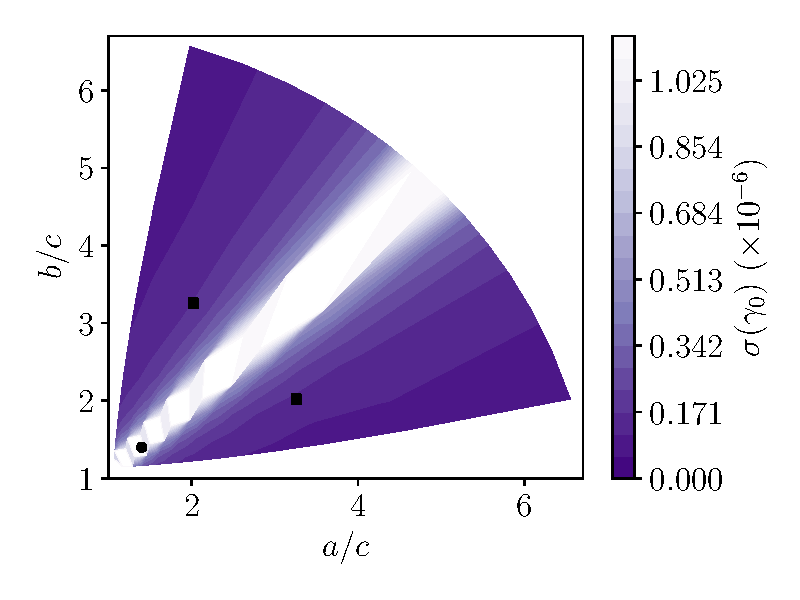
\includegraphics[width=0.3\textwidth]{figs/probe-space-ab-1-sigma.pdf}\hfill
  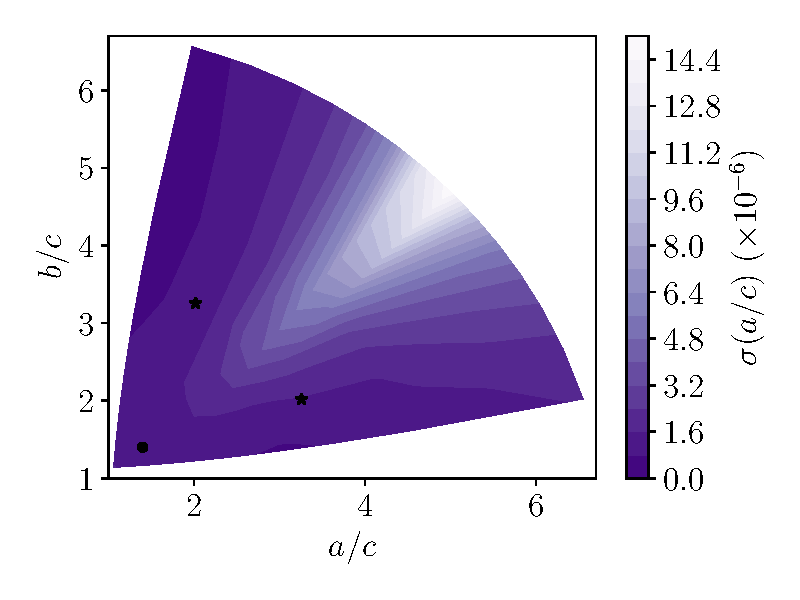
\includegraphics[width=0.3\textwidth]{figs/probe-space-ab-a-sigma.pdf}\hfill
  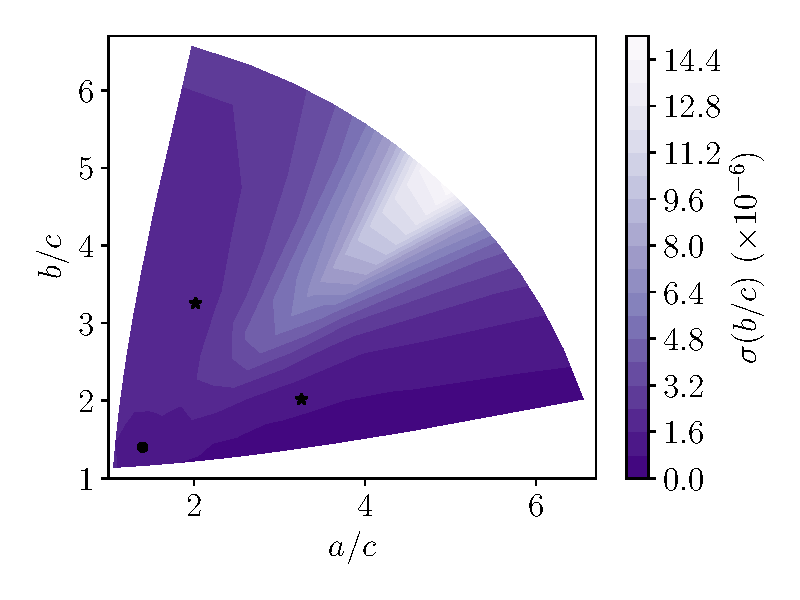
\includegraphics[width=0.3\textwidth]{figs/probe-space-ab-b-sigma.pdf}

  \caption{1$\sigma$ posterior uncertainty for first-order parameters $\gamma_0$, $K_{22}$, and $K_{20}$ (\textit{top row}) and $\gamma_0$, $a/c$, and $b/c$ (\textit{bottom row}). Also shown as black points are the reference asteroid shapes: symmetric (red circle) and asymmetric (black triangle). Symmetric asteroids ($K_{22}=0$ or $a/c=b/c$) show increased posterior uncertainty, but otherwise posterior uncertainty is roughly constant.}
  \label{fig:scan-space-sigma}
\end{figure*}

\begin{figure*}
  \centering
  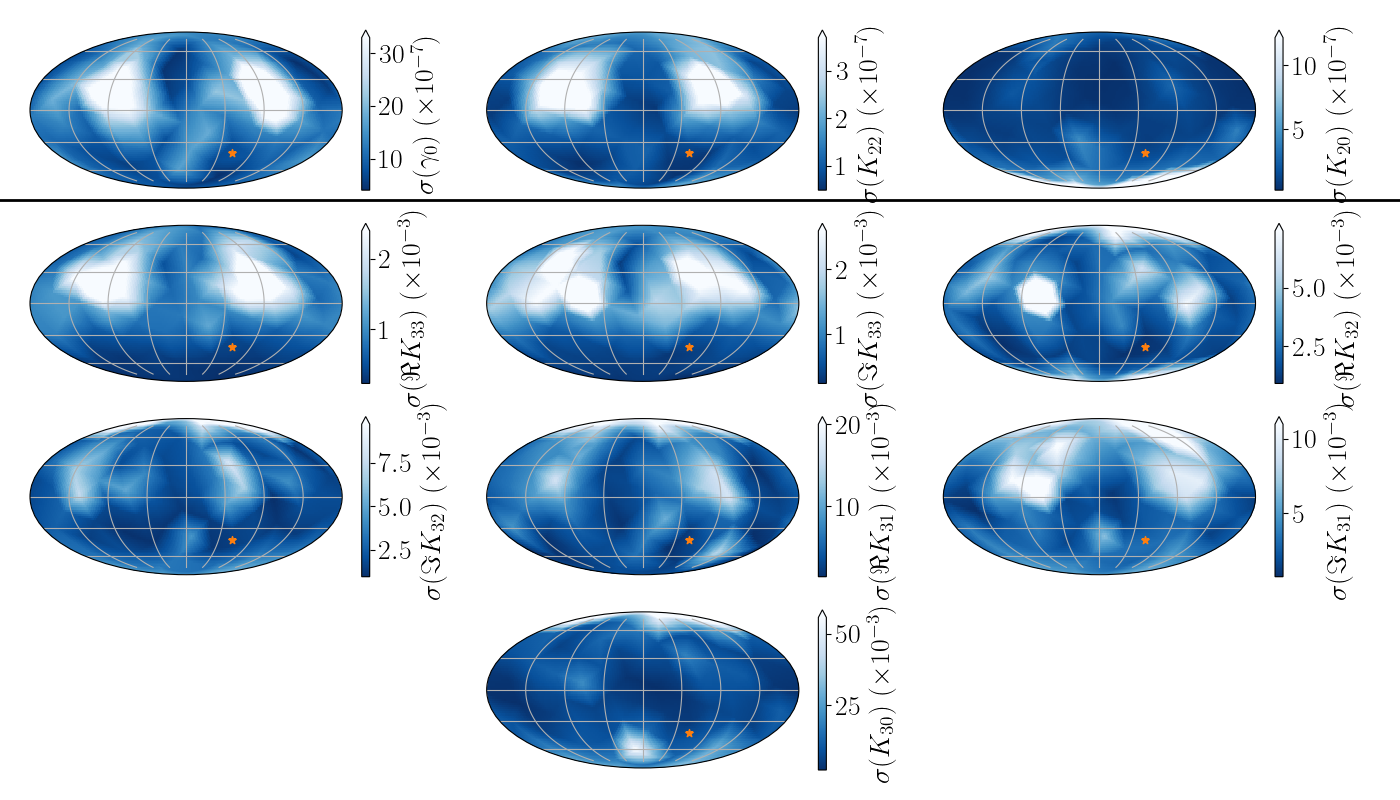
\includegraphics[width=0.8\textwidth]{figs/spin-pole.png}
  \caption{$1\sigma$ uncertainties for the first-order parameters (\textit{top}) and second-order (\textit{bottom}) as a function of the initial direction of spin in the inertial frame. All maps are made in the Mollweide projection. The orange star indicates the reference spin pole. The red contours enclose regions the 20\% (dotted) and 100\% (solid) $\sigma_\rho / \rho$ cut-off. Posterior uncertainty depends similarly on initial spin pole direction for all parameters}
  \label{fig:scan-spin}
\end{figure*}


Table \ref{tab:threshold-summary} reveals that the most limiting physical properties of the asteroid are its perigee and its length. \jtd{Further discuss}. Figure \ref{fig:scan-physical} demonstrates that the asteroid length cut-off is particularly sharp, since the density moment uncertainty $\sigma_{K_{3m}}$ is very steep there. However, precision on the moment of inertia ratios of the asteroid $K_{2m}$ are not affected by asteroid length; these may still be collected even for small asteroids.

The excess velocity and rotational period of the asteroid do not drastically affect the moment uncertainty and therefore do not impose strict thresholds, except for a dramatic increase in $\sigma(K_{2m})$ visible in figure \ref{fig:scan-physical} for rotational period $P_\omega \approx 4$ hr. The location of this threshold is likely dependent on other dynamical time scales of the system such as the cadence of observations and possibly the orbital time scales of $v_\infty / r_p$ and $\mu_\mathcal{A} / (v_\infty^2 r_p)$.

Physical parameters not studied here include the possibility of an initially tumbling asteroid and the presence of a third perturbing body, such as the Moon. Both are likely to increase precision but they are not within the scope of this paper.


The observational parameters also impose strict thresholds, most of all the uncertainty of the data set $\sigma_P / P$ and $\sigma_\rho$. Instantaneous rotational period uncertainty of less than one part in one million is required to resolve precise details of the asteroid density distribution. This could be accomplished by multiple, precise period measurements, increasing the time between observations to maximize the change in period between observations, increasing the data set to include more post-flyby tumbling data, or if necessary by increasing precision in the other observational parameters to relieve the burden on asteroid period. The instantaneous spin pole direction of the asteroid must also be known with precision on the order of degrees. However, the cadence of observations and the possibility of missing data points does not strongly affect results. Observations can be as much as 30 minutes apart and as much as 1.5 hr can be left out of the data set (equivalent to 45 missing data points for the reference 2 minute cadence), even during the high-torque perigee. The latter could be caused by the asteroid passing in front of the sun, for example. 

Two other properties important that affect moment uncertainty are the asteroid shape (as parametrized by the values of $K_{2m}$ or the axis lengths of the corresponding ellipsoid) and initial spin pole direction. The asteroid shape does not strongly affect density moment uncertainty, except that this model is not well-equipped to handle rotationally-symmetric asteroids with $K_{22} = 0$. For such asteroids, the principal axes can be selected to lie anywhere in the $xy$-plane, so that $\gamma_0$ is unconstrained. This inflates the moment uncertainties, although the density uncertainties are not badly affected as seen for the symmetric density distribution shown in figure \ref{fig:uniform}. A reparametrization of $\gamma_0$ would aid in decreasing moment uncertainty.


The initial spin pole of the asteroid also does not strongly affect the moment uncertainties, except when the initial spin pole happens to point perpendicular to the orbital plane, or in the plane and perpendicular to the major axis of the encounter. Both of these regions tend to result in less tidal torque, but even within these regions, the moment uncertainty generally is only double or triple that of other regions. 

Additional analysis of the data shown in this section, descriptions of how they were collected, and some supplementary figures are given in appendix \ref{app:uncertainty-dependence}.
                 


\subsection{Comparison of Jupiter and Earth encounters}
\label{sec:jupiter-earth}

If sufficiently accurate spin pole data can be detected for non-Earth encounters, it may be possible to extract density moments for encounters with larger planets. In this section, we run our reference asteroid through a Jupiter encounter to analyze the differences in uncertainty.

The physical parameters of the asteroid body are kept the same as the Earth encounter case (listed in appendix \ref{app:reference-configs}), as are the observational uncertainty and cadence. The orbit is adjusted for the Jupiter case by setting a perijove distance of $r_p=5$ Jupiter radii (compared to perigee radius $r_p=5$ Earth radii for the Earth encounter). The excess velocity does not strongly affect $\sigma(K_{\ell m})$ as shown in section \ref{sec:scan-orbit}, so we keep it at the reference value.
The ratio between the posterior uncertainties in the Jupiter and the Earth encounters are shown in table \ref{tab:jupiter-uncertainty}. In all cases, the Jupiter posteriors are more uncertain than Earth posteriors.

\begin{table}
  \centering
  \begin{tabular}{c|cc}
    \hline 
    $K_{\ell m}$ & $\sigma(K_{\ell m})_\text{Jupiter}/\sigma(K_{\ell m})_\text{Earth}$\\ \hline 
    $\gamma_0$ & 1.6 \\
    $K_{22}$ & 2.3 \\
    $K_{20}$ & 11 \\
    $\Re K_{33}$ & 18 \\
    $\Im K_{33}$ & 18 \\
    $\Re K_{32}$ & 18 \\
    $\Im K_{32}$ & 18 \\
    $\Re K_{31}$ & 25 \\
    $\Im K_{31}$ & 10 \\
    $K_{30}$ & 53 \\ \hline
  \end{tabular}
  \caption{Ratio of posterior uncertainty for all density moments $K_{\ell m}$ between an Earth encounter and a Jupiter encounter with identical properties except for an increased perigee. Observational uncertainty and cadence are assumed to be equivalent for the Jupiter and Earth encounters. Without taking the frequencies of close encounters into account, massive planets such as Jupiter yield less precise density moment estimates.}
  \label{tab:jupiter-uncertainty}
\end{table}

These uncertainty ratios can be understood as follows. The leading order of tidal torque is proportional to $\mu_\mathcal{A} / D^3$. If $D/a_\mathcal{B}$ (the ratio of the encounter distance to the central body radius) is roughly constant (as in this case, where $r_p/a_\mathcal{B}=5$), then $\mu_\mathcal{A} / D^3 \propto \rho_\mathcal{B}$ where $\rho_\mathcal{B}$ is the density of the central body. Therefore, little advantage is to be gained by looking for encounters of a massive planet in this sense. Since Jupiter is less dense than Earth, we expect that uncertainty in the first-order parameters $\gamma_0$ and $K_{2m}$ would be slightly worse than in the case of Earth, which is seen in table \ref{tab:jupiter-uncertainty}.

The second-order terms are damped by an additional factor of $a_\mathcal{A}/D$, which decreases if a massive central body is used. Since Jupiter is about 10 times larger in radius than Earth, we expect that the $K_{3m}$ terms are about ten times more uncertain than the $K_{2m}$ components, which is the case.

The $K_{\ell 0}$ components differ in that the posterior uncertainty increase for a Jupiter encounter over an Earth encounter is about five times greater for $K_{\ell 0}$ than other moments of the same $\ell$. In fact, $K_{30}$ essentially fills the prior. In section \ref{sec:scan-spin}, we noted that $K_{\ell 0}$ is particularly uncertain when the asteroid does not tumble after the perigee. In this case, the Jupiter encounter resulted in less tumbling than the Earth encounter, so the larger increase in uncertainty in $K_{\ell 0}$ shown in table \ref{tab:jupiter-uncertainty} is expected.

There are additional effects of central body mass which are not captured in this analysis. For example, encounters with massive planets are more plentiful, so that observation for a fixed period of time will lead to a larger number of observed encounters conducive to low-uncertainty moment extraction (large $a_\mathcal{A}$, small $r_p$, etc.). The distribution of $r_p$ in this encounter sample will also change; the ratio of the orbit impact parameter (the distance between the orbit asymptotes and the central body) to perijove distance is 
\begin{equation}
  \frac{b}{r_p} = \sqrt{1+2\frac{G\mu_\mathcal{B}}{r_p v_\infty^2}}.
\end{equation}
It was mentioned above that the observable perigee distance $r_p$ increases with $a_\mathcal{B} \sim \mu_\mathcal{B}^{1/3}$, so that $\frac{b}{r_p}$ is larger for more massive planets and therefore the same impact parameter leads to lower perijove. Other effects, such as a change in the physical properties of the encountering asteroids or decreased observational uncertainty due to the distance between Jupiter and Earth-based telescopes, may also affect the fit uncertainties. Which of these contradicting effects dominates is not immediately clear, and depends on the asteroid population near Jupiter and the observation method.



\subsection{Finite element model DOF}
\label{sec:dof-scan}
The number of elements $N$ used for the finite element model can be freely chosen. As discussed in section \ref{sec:finite-element}, seven of these are fixed by various constraints on the asteroid density distribution. There are 16 density moments with $\ell \leq 3$, so $N=16$ with nine DOF is the largest number of parameters the model can support. However, maximizing the DOF adds model-induced uncertainty to our results. This uncertainty can be reduced by reducing $N$, but with $N < 16$, a solution perfectly matching the extracted moments is not guaranteed. There is therefore a trade-off between the average density uncertainty $\sigma_\rho$ and the accuracy, which can be represented as the deviation of the density distribution from the true distribution $\Delta \rho$.

We investigate this trade-off by extracting five density distributions with five different finite-element layouts from moments extracted from synthetic data of the asymmetric reference asteroid. For each point in the asteroid, 1000 samples are drawn from each of the five density distributions. We use the standard deviation of the 5000 samples as the uncertainty $\sigma_\rho$ at that point, and the mean of the samples as the density $\rho$. Modelling the asteroid as having a uniform true density, we compute the deviation of the density from the truth $\Delta \rho$ over the asteroid. We do this for 9 (maximal), 7, 5, 3, and 2 DOF. Additionally, we vary the precision $\sigma_P$ of the data set used to extract the density moments, and plot $\sigma_\rho$ and $\Delta \rho$ as a function of $\sigma_P$. Figure \ref{fig:dof-scan} displays the distribution of $\sigma_\rho$, $\Delta \rho$, and the significance of the deviations from the truth ($\Delta \rho / \sigma_\rho$) over the asteroid.

\begin{figure}
  \includegraphics[width=\linewidth]{figs/dof-scan.pdf}
  \caption{The average uncertainty $\sigma_\rho$ and deviation from the truth $\Delta \rho$ of density distributions extracted by the finite element model with varying degrees of freedom. 5 DOF appears to optimize the trade-off between the model-induced uncertainty caused by too many DOF and the inaccuracy caused by too few.}
  \label{fig:dof-scan}
\end{figure}

The figure demonstrates the expected behaviour that few degrees of freedom results in low uncertainty but large $\Delta \rho / \sigma$, wile many degrees of freedom is more accurate but also more uncertain. The trend of uncertainty, deviation, and significance as a function of $\sigma_P$ is also discontinuous for few DOF, because in these cases the properties of the output distribution are strongly dependent on the initial choice of uncertainty of the initial choice of grids, and more than five grids are necessary to remove that dependence. This discontinuity is most noticeable for 3 and 2 DOFs, which also produce deviations from the true density distribution of the highest significance. We use 5 DOFs throughout this paper, produce the most precise results while still accurately reproducing the asteroid density distribution. 5 DOFs corresponds to $N=12$ finite elements.

The top panel of \ref{fig:dof-scan} also demonstrates that $\sigma_\rho$ reaches a plateau for large $\sigma_P$. In that regime, the prior constraints that the density of the asteroid take on physically meaningful values are more constraining than the actual data, leading to less dependence on the data quality. This is a further example of how the extracted asteroid density distribution is strongly dependent on the choice of model, and one of the reasons why we display the uncertainties of density moments in section \ref{sec:fit-uncertainty} rather than density distribution uncertainty. This moment uncertainty is not prone to the same model-dependent plateau.


\subsection{Comparisons between density distribution models}
\label{sec:density-compare}

In section \ref{sec:asym-density}, we displayed density distributions extracted via the lumpy model with $N=1$ lumps. When $N=1$, the model has two DOF, meaning that the density distribution can be determined only via the fit results for $K_{2m}$, rather than the relatively poorly constrained $K_{3m}$. Therefore, we also explore a density distribution with $N=2$ lumps, which has seven DOF.

\jtd{Continue}

\jtd{Possibly discuss moved core}

\section{Conclusions}

We derived a novel, arbitrary-order equation for the tidal torque experienced by an asteroid during an encounter with a planet of arbitrary shape and mass distribution. The tidal torque equation (equation \ref{eqn:tidal-torque}) revealed that the angular velocity of the asteroid over time depends strongly on $K_{\ell m}$ and the initial orientation. We then built a fast simulation for an asteroid encounter, truncating the equation at second-order, and used the simulation to extract first- and second-order density moments from synthetic spin pole data via a Markov Chain Monte Carlo fit. We observe the following general properties of the moments:
\begin{enumerate}
  \item The second-order moments $K_{3m}$ are roughly a factor of $~\frac{a_\mathcal{A}}{r_p}$ more uncertain than the first-order moments, where $a_\mathcal{A}$ is proportional to the asteroid radius and $r_p$ is the perigee distance. For our reference asteroid, this fraction was about $10^{-5}$.
  \item The second-order moments that measure small-scale variations in density (i.e., $|m|$ is large) are generally less uncertain. It is often possible to measure $K_{3|m|}$ for large $m$ even when $K_{30}$ is not resolved.
  \item Extracted density moments are generally more precise when the asteroid leaves the encounter tumbling.
  \item The oblateness of the central body cannot be ignored without generating incorrect density moment estimates.
\end{enumerate}

We assessed the posterior uncertainty generated by the fit process by adjusting various properties of an asteroid on an Earth encounter. The precise thresholds we measure (table \ref{tab:threshold-summary}) show that the observational uncertainty and perigee of the asteroid orbit are the most difficult requirements to meet, with perigee $\lesssim 6$ Earth radii, spin pole uncertainty $\lesssim 1^\circ$, and period uncertainty $\lesssim 10$ ms. However, these thresholds depend on the model used to extract a density distribution, and useful information may be able to be extracted when they are not achieved by using a different model.

Finally, we presented three fast, linear methods for extracting density distributions (together with uncertainties) from the density moments and the shape of the asteroid The extracted density distributions are largely consistent with the true distributions in all cases we tested. Slight adjustments to $K_{3m}$ dramatically change the overall distribution, so that they are not very precise. Indeed, the models sometimes predict negative density (though more complicated models could be made not to). Errors in the shape estimate of the asteroid also distort the density distribution, but the resulting distributions provide hints as to exactly where the shape is incorrect. Large-scale properties of the asteroid's true distribution, such as whether the mass is located in the middle or on the edges, are often observable. Two of the models presented (the harmonic and lumpy models) are flexible in their number of parameters, so that if only these large-scale properties are necessary, a small set of parameters can be chosen to prevent over-fitting.`'

\section*{Acknowledgements}

We warmly thank Emmanuel Jehin, Maxime Devogele, and Marin Ferrais for meeting with the authors to discuss this work and pointing out possible future initiatives. JTD also thanks the MIT UROP office for funding his work. This paper made substantial use of MIT Supercloud's facilities.



%%%%%%%%%%%%%%%%%%%%%%%%%%%%%%%%%%%%%%%%%%%%%%%%%%
\section*{Data Availability}

The asteroid simulation, fit process, and density moment extraction code are available on \href{https://github.com/jack-dinsmore/asteroid-tidal-torque}{GitHub}.



%%%%%%%%%%%%%%%%%%%% REFERENCES %%%%%%%%%%%%%%%%%%

\bibliographystyle{mnras}
\bibliography{asteroids.bib}



%%%%%%%%%%%%%%%%%%%%%%%%%%%%%%%%%%%%%%%%%%%%%%%%%%

%%%%%%%%%%%%%%%%% APPENDICES %%%%%%%%%%%%%%%%%%%%%

\appendix

\section{Tidal torque \& Equations of motion}
\label{app:eom}

In this appendix, we derive the equations of motion used to simulate the asteroid angular velocity during the encounter. In particular, we describe our coordinates (section \ref{sec:coordinates}) for an encountering asteroid's position and orientation, and we parametrize its density distribution via its density moments (section \ref{sec:moments}). Then we derive an arbitrary-order equation for tidal torque (section \ref{sec:tidal-torque}) and write the equations of motion for the system (section \ref{sec:eom}).

\subsection{Coordinates}
\label{sec:coordinates}

We make use of two frames of reference to model this system. One is the ``inertial frame,'' with axes denoted by $\unit{X}$, $\unit{Y}$, $\unit{Z}$ and origin placed at the central body's centre of mass. $\unit{X}$ points from the central body to the asteroid periapse, and $\unit{Z}$ points parallel to the orbit angular momentum. We assume that the mass distribution of the central body is known in this inertial frame.

Our second frame is the ``body-fixed'' frame, denoted by $\unit{x}, \unit{y}, \unit{z}$. Each axis in this frame is aligned with a principal axis and rotates with the asteroid, with its origin at the asteroid's centre of mass. For definiteness, we define $\unit{z}$ to be the principal axis with maximal MOI (this is the short axis mode, to use the vocabulary of Ref.~\cite{kaasalainen2001interpretation}). In general, we use capital letters to denote vectors in the inertial frame and lowercase vectors to denote vectors in the body-fixed frame.

The difference between the origins of the body-fixed and inertial frames is the position of the asteroid. We represent the relative orientations by $z-y-z$ Euler angles $\alpha$, $\beta$, and $\gamma$, such that a matrix $M$ rotating from the body-fixed to the inertial frame ($M\bm{r} = \bm{R}$) is given by
\begin{equation}
M = R_z(\alpha) R_y(\beta) R_z(\gamma).
\label{eqn:euler-angles}
\end{equation}
Here, $R_i(\theta)$ is a rotation around the unit vector $i$ by $\theta$ (figure \ref{fig:euler-angles}).

\begin{figure}
    \centering
    \begin{tikzpicture}
    \draw[-{Latex[length=3mm]}] (0, 0) -- (-4, 0) node[anchor=east] {$\unit x$};
    \draw[-{Latex[length=3mm]}] (0, 0) -- (2, -3) node[anchor=west] {$\unit y$};
    \draw[-{Latex[length=3mm]}] (0, 0) -- (0, 4) node[anchor=south] {$\unit z$};
    \draw[dashed, -{Latex[length=3mm]}] (0, 0) -- (3.7, -2) node[anchor=north] {};
    \draw[line width=0.5mm,-{Latex[length=3mm]}] (0, 0) -- (-0.5, -3) node[anchor=north] {$\unit X$};
    \draw[line width=0.5mm,-{Latex[length=3mm]}] (0, 0) -- (4, 1) node[anchor=south] {$\unit Y$};
    \draw[line width=0.5mm,-{Latex[length=3mm]}] (0, 0) -- (-1.6, 2.7) node[anchor=south] {$\unit Z$};
    \draw[->] (0.5, -0.75) arc (290:302:2.5);
    \draw (0.9, -0.9) node[anchor=center] {$\alpha$};
    \draw[->] (0, 1.2) arc (130:161:1.3);
    \draw (-0.3, 1.3) node[anchor=center] {$\beta$};
    \draw[->] (0.97, -0.52) arc (330:368:1.3);
    \draw (1.4, -0.25) node[anchor=center] {$\gamma$};
    %\draw[-{Latex[length=3mm]}] (0, 0) -- (0, 4) node[anchor=south] {$\unit Z$};
    %\draw[-{Latex[length=3mm]}] (0, 0) -- (4, 0) node[anchor=west] {$\unit Y$};
    %\draw[-{Latex[length=3mm]}] (0, 0) -- (-2, -2) node[anchor=east] {$\unit X$};
    \end{tikzpicture}
    \caption{$z-y-z$ Euler angles used in this work to express the orientation of the asteroid. Orientation is expressed as a rotation from the body-fixed axes (lowercase) to the inertial axes (bold lines and uppercase). The origins are co-located for demonstration purposes.}
    \label{fig:euler-angles}
\end{figure}


\subsection{Density moments}
\label{sec:moments}

The un-normalized spherical harmonics are defined as $Y_{\ell m}(\theta, \phi) = P_{\ell m}(\cos \theta)e^{im\phi}$, where $P_{\ell m}$ are the associated Legendre Polynomials without the Condon-Shortley phase. The regular and irregular spherical harmonics are further defined as
\begin{equation}
  \begin{split}
    S_{\ell m}(\bm r) &= (-1)^m (\ell - m)! \frac{Y_{\ell m}(\unit r)}{r^{\ell+1}} \\
    R_{\ell m} (\bm r) &= (-1)^m \frac{r^\ell}{(\ell + m)!} Y_{\ell m}(\unit r).
  \end{split}
\end{equation}
These spherical harmonics obey many useful identities summarized in Ref.~\cite{Gelderen1998TheSO}, which are also useful for quantum mechanics. They were used to define the density moments in equation \ref{eqn:klm}, which can be extended to the central body:
\begin{equation}
  \begin{split}
    &J_{\ell m} = \frac{a_\mathcal{B}^{2-\ell}}{I_\mathcal{B}} \int_\mathcal{B} d^3 r \rho_\mathcal{B}(\bm r) R_{\ell m}(\bm r)\\
  \end{split}
  \label{eqn:jlm}
\end{equation}
By contrast, $J_{\ell m}$ should be computed in the inertial frame. The length scale $a_\mathcal{B}$ and MOI scale $I_\mathcal{B}$ can be defined similarly to $a_\mathcal{A}$ and $a_\mathcal{B}$ in equations \ref{eqn:aa} and \ref{eqn:ia}, but they could also be set to any other scales of the same units, e.g. $a_\mathcal{B}$ equal to the central body radius and $I_\mathcal{B} = \mu_\mathcal{B}a_\mathcal{B}^2$, where $\mu_\mathcal{B}$ is the central body mass.

Note that both $J_{\ell m}$ and $K_{\ell m}$ are unitless. We call them ``moments'' because the $R_{\ell m}(\bm r)$ contains an $r^\ell$ dependence so that $K_{\ell m}$ is the $\ell$th density moment of the asteroid.

These moments share several key properties which we discuss before continuing. Firstly, for real mass density, properties of the spherical harmonics imply that $K_{\ell m} = (-1)^m K_{\ell, -m}^*$. Therefore, the set of $K_{\ell m}$ for $\ell < \ell_\text{max}$ contains $\ell_\text{max}^2$ degrees of freedom. However, some of these degrees of freedom are redundant with the choice of coordinates: $K_{1m} = 0$ since the body-fixed frame is centred on the asteroid centre of mass. Further calculation reveals that the alignment of the body-fixed frame with the asteroid principal axes also forces $K_{21}= 0$ and $\Im K_{22}=0$. The only physical density moments for $\ell \leq 2$ are therefore $K_{22}$, $K_{20}$, and $K_{00}$. The first two are related to the MOI around each principal axis by equation \ref{eqn:moi}, while $K_{00} = \mu_\mathcal{A} a_\mathcal{A}^2 / I_\mathcal{A}$ will not be relevant to this study as it does not appear in equation \ref{eqn:tidal-torque}. 

The physical meaning of $K_{22}$ and $K_{20}$ can also be interpreted via a special case: if the asteroid is a uniform-density triaxial ellipsoid, the moments of inertia are simple to compute in terms of the semi-axis lengths and can be compared to those found in equation \ref{eqn:moi}. This yields semi-axis lengths of 
\begin{equation}
  \begin{split}
  a &= \sqrt{\frac{5}{3}}a_\mathcal{A}\sqrt{1-2K_{20}+12K_{22}}\\
  b &= \sqrt{\frac{5}{3}}a_\mathcal{A}\sqrt{1-2K_{20}-12K_{22}}\\
  c &= \sqrt{\frac{5}{3}}a_\mathcal{A}\sqrt{1+4K_{20}}.
  \label{eqn:ellipsoid-axes}
  \end{split}
\end{equation}
The higher-order moments $K_{3m}$ can be thought of loosely as measuring the large-scale asymmetries of the asteroid. An asteroid that is mirror-symmetric along the $\unit{x}$ axis (meaning $\rho_\mathcal{A}(x,y,z)=\rho_\mathcal{A}(-x,y,z)$) necessarily sets certain density moments to zero. Which density moments are zeroed by which mirror symmetries is outlined in table \ref{tab:klm-symmetries}. All $K_{3m}$ are zeroed by at least one mirror symmetry. 

\begin{table}
  \centering
  \begin{tabular}{c|ccccccc}
    \hline
    $\ell$ & $\Re K_{\ell 3}$ & $\Im K_{\ell 3}$ & $\Re K_{\ell 2}$ & $\Im K_{\ell 2}$ & $\Re K_{\ell 1}$ & $\Im K_{\ell 1}$ & $K_{\ell 0}$ \\ \hline
    0 &  &  &  &  &  &  & -\\ 
    1 &  &  &  &  & x & y & z\\ 
    2 &  &  & - & x,y & y,z & x,z & -\\ 
    3 & x,z & y,z & z & x,y,z & x & y & z\\ \hline
  \end{tabular}
  \caption{Axes of mirror symmetry that imply zeroed density moments. For example, for mirror symmetries along $\unit y$ or $\unit z$, $\Im K_{32}=0$. Mirror symmetry along $\unit x$ means $\rho_\mathcal{A}(x, y, z) = \rho_\mathcal{A}(-x, y, z)$. Dashes indicate that none of the mirror symmetries zero the moment in question. Since $r^2>0$ for $r\neq 0$, no symmetries set $a_\mathcal{A}=0$ either.}
  \label{tab:klm-symmetries}
\end{table} 

Finally, the requirement that $\rho_\mathcal{A}(\bm r) \geq 0$ everywhere restricts $K_{\ell m}$. In the case of $K_{2m}$, this fact and the constraint that $I_z$ is larger than $I_x$ or $I_y$ requires $K_{20}$ and $K_{22}$ to fall in the triangle
\begin{equation}
  -\frac{1}{4} \leq K_{20} \leq 0, \qquad |K_{22}| \leq -\frac{K_{20}}{2}.
  \label{eqn:parameter-bounds}
\end{equation}
An analytical constraint on $K_{3m}$ based on this property is more difficult to derive, but in practice, we also observe that $|K_{3m}| < 0.01$.




\subsection{Tidal torque}
\label{sec:tidal-torque}

Derivations for the tidal torque experienced by a rigid body in the gravitational field of a larger mass have been computed by several previous studies \cite{paul88,HouMar2017,BOUE2009750, ashenberg07}, often in terms of the MOI of the rigid body (or higher order moments of inertia), and to varying degrees of precision. A simple, first-order derivation is also easily computable in terms of the asteroid MOI in the inertial frame.

Here, we present a new derivation of the tidal torque to arbitrary orders in terms of the density moments of an asteroid defined in section \ref{sec:moments}. These density moments can be pre-computed and do not have to be re-evaluated every time-step.

The gravitational potential energy of the central body is, in its most general form,
\begin{equation}
V(\bm R') = -G\int_\mathcal{B} d^3 R \rho_\mathcal{B}(\bm R) \frac{1}{|\bm{R}-\bm{R'}|}.
\label{eqn:first-pe}
\end{equation}
where $\rho_\mathcal{B}$ is the density distribution of the central body and $\mathcal{B}$ indicates the central body's volume. All vectors here are written in the inertial frame. Given $|\bm{R}| < |\bm{R'}|$, Ref.~\cite{Gelderen1998TheSO} gives the identity
\begin{equation}
  \frac{1}{|\bm R - \bm R'|} = \sum_{\ell, m} R_{\ell m}(\bm R) S_{\ell m}^*(\bm R'),
  \label{eqn:ylm-expansion}
\end{equation}
where the sum is shorthand for $\sum_{\ell, m} = \sum_{\ell = 0}^\infty \sum_{m=-\ell}^\ell$.

Incidentally, it is the $|\bm R| < |\bm R'|$ assumption that inspires the assumption that there are ``no \textit{distant} perturbing objects'' (section \ref{sec:methods}). If a perturbing object such as a moon is not distant (i.e., it is closer to the system center of mass than the asteroid perigee so that $|\bm R| < |\bm R'|$ always), then it can be absorbed into $J_{\ell m}$ by equation \ref{eqn:jlm} and the assumptions of this derivation are not violated.

We are interested in translating the potential energy of equation \ref{eqn:first-pe} to the body-fixed frame. To do this, we let $\bm{R'} = \bm D + \bm U$, where $\bm D$ is the location of the asteroid in the inertial frame. We further define $\bm U = M\bm u$, where $\bm u$ is in the body-fixed frame and $M$ is the rotation matrix given by the Euler angles $\alpha$, $\beta$, and $\gamma$ (see section \ref{sec:coordinates}). The translation from $\bm {R'}$ to $\bm U$ is then attained by the identity 
\begin{equation}
  S_{\ell m}(\bm R') = \sum_{\ell', m'} (-1)^{\ell'}R^*_{\ell' m'}(\bm U)S_{\ell+\ell', m + m'} (\bm D),
  \label{eqn:ylm-translation}
\end{equation}  
provided by Ref.~\cite{Gelderen1998TheSO}, and from $\bm U$ to $\bm u$ is given by
\begin{equation}
  \begin{split}
    Y_{\ell m}(M\bm u) = \sum_{m'=-\ell}^\ell & (-1)^{m+m'}\sqrt{\frac{(\ell-m')!(\ell+m)!}{(\ell+m')!(\ell-m)!}} \\
    & \times \mathcal{D}^\ell_{mm'}(M)^* Y_{\ell m'}(\bm u).\\
  \end{split}
  \label{eqn:ylm-rotation}
\end{equation}
Here, $\mathcal{D}^\ell_{mm'}(M)$ are the Wigner-$D$ matrices, which are determined by the Euler angles $\alpha$, $\beta$, and $\gamma$ of $M$.

Equations \ref{eqn:first-pe} to \ref{eqn:ylm-rotation} then provide formula for $V(\bm u)$ expressed as a sum of integrals over $\mathcal{B}$ of the central body density $\rho_\mathcal{B}(\bm R)$ times $R_{\ell m}(\bm R)$. These are expressed via equation \ref{eqn:jlm} as $J_{\ell m}$.

The tidal torque experienced by the asteroid (in the body-fixed frame) is given by
\begin{equation}
  \bm{\tau}(\bm u) = \int_\mathcal{A} d^3 u \rho_\mathcal{A}(\bm u) (\bm u \times (-\nabla_{\bm u} V(\bm u)))
\end{equation}
where $\rho_\mathcal{A}$ is the density distribution of the asteroid and $\mathcal{A}$ indicates the volume of the asteroid. Making use of one more identity concerning the derivatives of spherical harmonics:
\begin{equation}
  \begin{split}
  \bm u \times \nabla R_{\ell m}(\bm u)=&\frac{1}{2}\Big[(i\unit x - \unit y)(\ell-m+1)R_{\ell,m-1}(\bm u)\\
  &+(i\unit x+\unit y)(\ell+m+1)R_{\ell,m+1}(\bm u)\\
  & +2im\unit z R_{\ell m}(\bm u)\Big],
  \end{split}
\end{equation}
tidal torque can now be expressed as a function only of the constants $J_{\ell m}$, $K_{\ell m}$, $a_\mathcal{A/B}$, $I_\mathcal{A/B}$, and the asteroid orientation and position (equation \ref{eqn:tidal-torque}). Some $K_{\ell m}$ terms are written in this equation with $|m|>\ell$; these should all be taken to be zero.

\subsection{Equations of motion}
\label{sec:eom}


The equations of motion of the asteroid position $\bm D$ are given by Newton's law of gravitation
\begin{equation}
  \dot{\bm V} = -\frac{G \mu_\mathcal{B}}{D^3} \bm D \qquad \dot{\bm D} = \bm V
  \label{eqn:pos-eom}
\end{equation}
where $\bm V$ is the asteroid velocity in the inertial frame. Rather than derive equations of motion for the Euler angles (which suffer from gimbal lock), we instead represent the orientation of the asteroid with a quaternion $\quat q$ which can be converted into Euler angles to compute $\mathcal{D}(\alpha, \beta, \gamma)$. This quaternion evolves as 
\begin{equation}
  \dot{\quat q} = \frac{1}{2}\quat q\quat \omega.
  \label{eqn:quat-eom}
\end{equation}
for angular velocity $\bm \omega$ given in the body-fixed frame. The equations of motion of $\bm \omega$ in turn are given by
\begin{equation}
  \begin{split}
    I_x \dot \omega_x - \omega_y \omega_z (I_y - I_z) &= \tau_x\\
    I_y \dot \omega_y - \omega_z \omega_x (I_z - I_x) &= \tau_y\\
    I_z \dot \omega_z - \omega_x \omega_y (I_x - I_y) &= \tau_z.
  \end{split}
  \label{eqn:omega-eom}
\end{equation}
Equations \ref{eqn:tidal-torque}, \ref{eqn:moi}, and \ref{eqn:pos-eom} to \ref{eqn:omega-eom} form a set of non-linear, first-order coupled differential equations in which can be numerically integrated. They are expressed in terms of the physical parameters $I_\mathcal{A/B}$, $a_\mathcal{A/B}$, $J_{\ell m}$, and $K_{\ell m}$ which are constant if the asteroid is rigid and the central body does not rotate.






\section{Comparing orientation and angular velocity data}

To extract the density distribution of an asteroid, the main text assumes that the angular velocity data of the asteroid is observable. It is possible that the orientation of the asteroid may be better constrained by observations than angular velocity. In this appendix, we generate an orientation data set for the reference asteroid flyby, extract a density distribution from it, and compare the results to distributions extracted from angular velocity data.

\subsection{Uncertainty model}
The likelihood used by the MCMC (equation \ref{eqn:log-likelihood}) requires redefinition in order to extract density moments from orientation data. This requires a new model for the uncertainty of orientation observations.

For the sake of this appendix, we will assume that all observations of orientation $O$ differ from the true orientation $O^*$ by a rotation by some angle $\phi$ around an axis drawn from a uniform distribution on the unit sphere, where $\phi$ is drawn from a normal distribution with mean zero and standard deviation $\sigma_\phi$. Expressing orientation as a quaternion $\quat q = q_r + q_i \bm i + q_j \bm j + q_k \bm k$, $\phi$ can be extracted and the likelihood written as 
\begin{equation}
  \ln \mathcal{L} = -\frac{2}{\sigma_\phi^2}\sum_{i=0}\parens{\cos^{-1}\left|\brackets{\quat q_i (\quat q_i^*)^{-1}}_r\right|}^2
  \label{eqn:orientation-like}
\end{equation}
where $\quat q_i$ is the $i$th quaternion in the data set measured in the inertial frame, and $\quat q_i^*$ is the true quaternion. It is assumed that both quaternions have norm one.

\subsection{Moment uncertainty comparison}
With the likelihood defined, we generate both angular velocity and orientation data for the asymmetric reference asteroid configuration and extract $K_{\ell m}$ means and uncertainties for both data sets via the fit method defined in the main text. Due to the different uncertainty models used for the orientation and angular velocity data sets, this set-up does not allow direct comparison between the sizes of moment uncertainty for both data sets. If one data set yields more precise moments than the other, one could not determine whether the effect is due to increased observational precision in the data set or the use of a data type that better constrains density moments. However, the relative uncertainty of moments can be compared between the two data sets.

To make this comparison, we compute moment uncertainties $\sigma(K_{\ell m})$ for both data sets and also compute the mean value of $\sigma(K_{\ell m})$ over all fit parameters. We then scale the moment uncertainties attained from the angular velocity data set so that the mean uncertainty of its parameters is equal to that of the orientation data set. This is equivalent to simply choosing observational uncertainties for the angular velocity data set which yield density moments to the same precision as the observational data set, because figure \ref{fig:scan-observational} shows that density moment uncertainty $\sigma(K_{\ell m})$ is proportional to observational uncertainty. The resulting PPDs for the density moments of both data sets are displayed in figure \ref{fig:orientation-unc}, as well as their mean values relative to the true values.

\begin{figure}
  \centering
  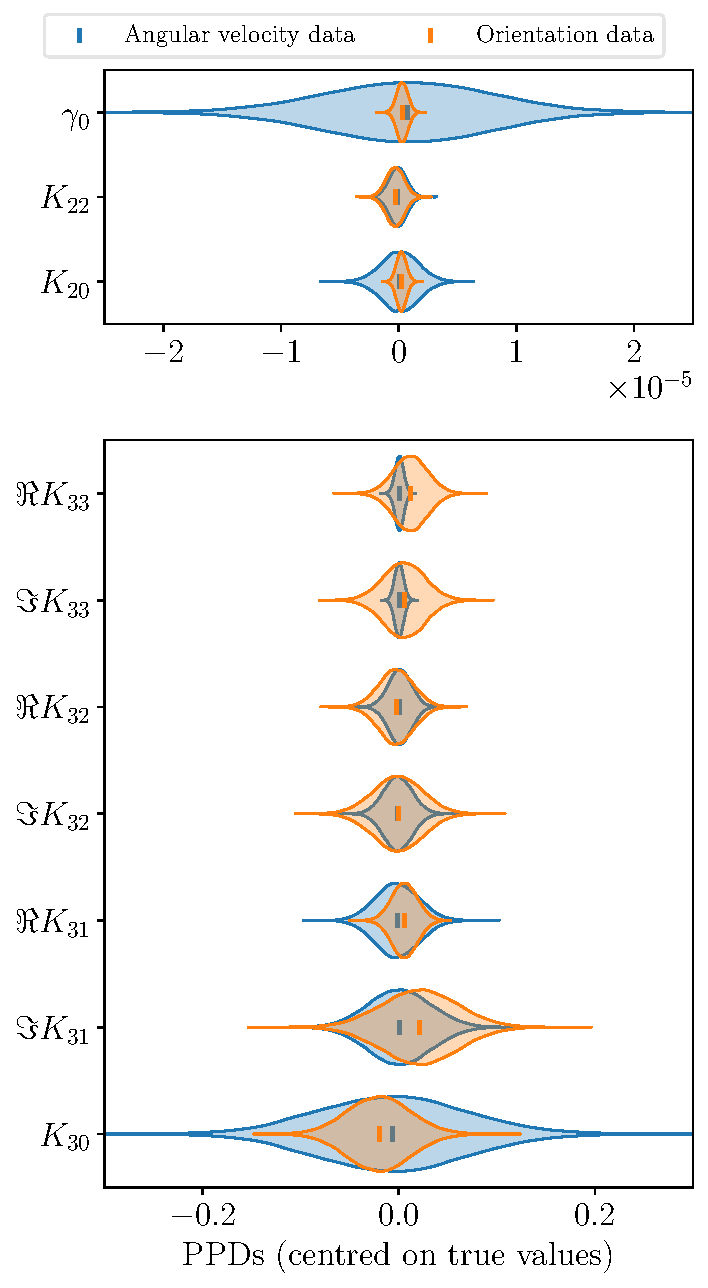
\includegraphics[width=0.7\linewidth]{figs/orientation-unc}
  \caption{PPDs for each parameter as extracted from angular velocity (blue) and orientation (orange) data. First order parameters are shown in the top panel and second-order parameters in the bottom. Mean values are also shown as vertical lines. Both data produce similar constraints on parameters, except in the case of $\gamma_0$.}
  \label{fig:orientation-unc}
\end{figure}

The figure demonstrates that using orientation data rather than angular velocity data does not greatly affect the relative uncertainties of density moments, except in the case of $\gamma_0$. This is expected due to the following argument. If the initial orientation of the asteroid is known, then the orientation of the next data point can be determined by knowledge of the asteroid's angular velocity at that moment. Thus, an orientation data set can be produced from an angular velocity data set and vice versa given an initial asteroid orientation. This initial orientation is defined up to $\gamma_0$ by the assumption of no initial tumbling, so that the orientation data set will affect $\sigma(\gamma_0)$ most strongly.

A smaller effect observed in figure \ref{fig:orientation-unc} is that the orientation data set yields similar uncertainties for all density moments of fixed $\ell$, whereas the angular velocity data set tends to yield larger uncertainties for small $|m|$, which will alter the density uncertainty discussed in the next section. However, this has little effect on the density distributions extracted by the finite element model from the two PPDs shown in the figure. The average density uncertainty $\sigma_\rho / \rho$ are essentially equivalent between the two data sets, as is the distribution of density and density uncertainty extracted.




\section{Additional density distribution models}
\label{app:more-models}

Two models were discussed in section \ref{sec:density-distro} to translate density moment constraints into density distribution constraints. Here we outline two additional models, the nearly-uniform and the harmonic models, which are less conventional but still useable for extracting density distribution properties. Unlike the finite element and lumpy models discussed in the main text, these models will yield smooth distributions with no discrete transitions. They also rely on a known surface for the asteroid.

\subsection{Nearly-uniform model}
In this ``nearly-uniform'' model, we seek to pick one density distribution from the many distributions consistent with the data by maximizing a prior distribution $f[\rho(\bm r)]$, which can be chosen manually. Any prior distribution can be chosen, but the following prior is both interesting and numerically efficient.

As part of our prior, we require that the asteroid density distribution satisfy $I_\mathcal{A} = \mu_\mathcal{A} a_\mathcal{A}^2$. This constraint is desirable as it is obeyed for uniform density distributions. To define the prior, we divide the asteroid into $n \gg 1$ small regions of volume $V$, each with position $\bm r_i$ and density $\rho_i = \delta_i + 1$. Setting the mass of the asteroid equal to its volume, the average density is 1, so $\delta_i$ is the difference between the average and local density. We set $f[\rho(\bm r)]$ to be a multivariate-Gaussian distribution on $\delta_i$, centred on zero to minimize non-uniformity, i.e.
\begin{equation}
  f[\rho(\bm r)] \propto \prod_i \exp\parens{-\frac{\delta_i^2}{2\sigma^2}} \implies \ln f[\rho(\bm r)] \simeq -\sum_i \delta_i^2
  \label{eqn:nu-f}
\end{equation}
where $\sigma$ is an irrelevant constant. The density moments, MOI scale, and mass are 
\begin{equation}
  K_{\ell m} = \frac{V}{\mu_\mathcal{A}a_\mathcal{A}^{\ell}} \sum_i (\delta_i + 1) R_{\ell m}(\bm r_i)
  \label{eqn:nu-klm}
\end{equation}
\begin{equation}
  I_\mathcal{A} = \mu_\mathcal{A} a_\mathcal{A}^2 = V \sum_i (\delta_i + 1) r_i^2
  \label{eqn:nu-ia}
\end{equation}
\begin{equation}
  \mu_\mathcal{A} = V\sum_i (\delta_i + 1) \implies 0 = \sum_i \delta_i.
  \label{eqn:nu-mass}
\end{equation}
Writing $\delta_i$ as an $n$-dimensional vector $\bm \delta$, equation \ref{eqn:nu-klm} is a matrix equation for $K_{\ell m}$, and equations \ref{eqn:nu-ia} and \ref{eqn:nu-mass} are vector dot product equations. Combining $K_{\ell m}$, $I_\mathcal{A}$, and $0$ into a single vector $\bm K$, these equations can be written as a single underdetermined matrix equation we denote as 
\begin{equation}
  \bm K = M \bm \delta + \bm C,
  \label{eqn:nu-matrix}
\end{equation}
where the components of constant matrix $M$ and constant vector $\bm C$ are known given a fixed layout of the $n$ regions. Some of the components of $\bm K$, such as $I_\mathcal{A}$, $\mu_\mathcal{A}$, and $K_{1m}$, are constraints. We treat the other components as parameters of the model. The task is then to find $\bm \delta$ that satisfies equation \ref{eqn:nu-matrix} and maximizes $f(\bm \delta)$. But the form of equation \ref{eqn:nu-f} shows that the maximum of $\ln f$ (also the maximum of $f$) is the minimum of $|\bm \delta|^2$. This shortest value of $\bm \delta$ that obeys equation \ref{eqn:nu-matrix} is given by the Moore-Penrose inverse:
\begin{equation}
  \bm \delta = M^+ (\bm K - \bm C); \qquad M^+ = M^\dagger(M M^\dagger)^{-1}
  \label{eqn:nu-delta}
\end{equation}
where $M^\dagger$ is the adjoint of $M$.

The prior distribution on $\rho(\bm r)$ discussed in section \ref{sec:fit} can be implemented by individually checking the components $\bm \delta$ computed by equation \ref{eqn:nu-delta} and confirming that $1 + \delta_i$ lies within the acceptable range of densities.
 can be implemented by individually checking the components $\bm \delta$ computed by equation \ref{eqn:nu-delta} and confirming that $1 + \delta_i$ lies within the acceptable range of densities.


\subsection{Harmonic model}
This the ``harmonic model'', we limit ourselves to density distributions that are harmonic; i.e., they satisfy $\nabla^2 \rho(\bm r) = 0$. We have no physical justification for why this assumption should be true, but it is useful as a simplification to gain qualitative insight into the properties of the asteroid density distribution.

A harmonic density distribution can be expanded in terms of the spherical harmonics as $\rho(\bm r) = \sum_{\ell m} C_{\ell m} R_{\ell m}(\bm r)^*$ where $C_{\ell m}$ are complex, free parameters. This series can be truncated at some maximum $\ell$. The density moments, MOI scale, and mass can then be explicitly computed as a function of $C_{\ell m}$:
\begin{equation}
  K_{\ell m} = \frac{a_\mathcal{A}^{2-\ell}}{I_\mathcal{A}} \sum_{\ell m} C_{\ell' m'} \int_\mathcal{A} d^3 r R_{\ell' m'}(\bm r)^* R_{\ell m}(\bm r)
  \label{eqn:harmonic-klm}
\end{equation}
\begin{equation}
  I_\mathcal{A} = \sum_{\ell m} C_{\ell m} \int_\mathcal{A} d^3 r R_{\ell m}(\bm r)^* r^2
  \label{eqn:harmonic-ia}
\end{equation}
\begin{equation}
  \mu_\mathcal{A} = \sum_{\ell m} C_{\ell m} \int_\mathcal{A} d^3 r R_{\ell m}(\bm r)^*.
  \label{eqn:harmonic-mass}
\end{equation}
These integrals can be pre-computed given a known asteroid shape $\mathcal{A}$, so that computing $C_{\ell m}$ to match a given $K_{\ell m}$ is fast. Furthermore, their values when $\mathcal{A}$ is spherical gives us insight into the influence of $K_{\ell m}$ on density distributions. In this case, $I_\mathcal{A} \propto C_{00}$ and the integral of equation \ref{eqn:harmonic-klm} is non-zero only when $\ell' = \ell$ and $m'=m$. Therefore, $C_{\ell m}$ is proportional to $K_{\ell m}$. The density distribution can be immediately visualized given the density moments as a sum of the solid spherical harmonics weighted by $K_{\ell m}$. When the asteroid is non-spherical, the shape itself contributes to $K_{\ell m}$ so as to break this picture.

Imposing constraints on these moments is also necessary. The choice of mass is enforced via equation \ref{eqn:harmonic-mass}. We impose bounds on $\rho(\bm r)$ by acknowledging that harmonic functions such as $\rho(\bm r)$ in a region such as $\mathcal{A}$ attain their maxima on the boundary of the region, so that it is only necessary to ensure that $\rho$ lies within the allowed range on the asteroid boundary rather than within the entire asteroid. This can be done by parametrizing the asteroid surface as a function of two variables (e.g., latitude and longitude) and minimizing and maximizing $\rho$ with respect to those variables, ensuring these minima and maxima are within the allowed range.







% \section{Dependence of the cadence cut-off on time scales}
% \label{app:cadence-tests}

% In section \ref{sec:scan-cadence}, we noted that moment uncertainty as a function of observation cadence $\Delta t$ increases suddenly near $\Delta t_\text{cut-off} \approx 30-40$ min. By dimensional analysis, $\Delta t_\text{cut-off}$ depends both on the asteroid period $P_\omega$ and the orbital time scales. In this appendix, we assess the relationship between $\Delta t_\text{cut-off}$ and these time scales by measuring moment uncertainty as a function of cadence at different values of these time scales. However, changing the time scales also affects the moment uncertainty directly, obscuring the cadence dependence of the moment uncertainty. Figure \ref{fig:scan-period} indicates that $P_\omega$ only slightly affects moment uncertainty as long as $P_\omega$ is not too small, so we neglect this obscuring effect in the case of $P_\omega$. To assess the dependence of $\Delta t$ on the orbital time scales, we fix the orbit shape and simulate the asteroid as following the orbit at different speeds. This process is unphysical, but it has the advantage of keeping all encounter parameters fixed except for the time the asteroid spends in the orbit, thereby isolating the orbital time scale. We parametrize this change $v_\text{orbit} / v_\text{physical}$, which is large for an artificially fast encounter, low for an artificially slow encounter, and 1 for a physical encounter.

% In figure \ref{fig:cad-contour}, we display contour plots of moment uncertainty $\sigma(K_{\ell m})$ of the fit parameters as a function of both cadence $\Delta t$ and $P_\omega$ and the relative orbit speed $v_\text{orbit} / v_\text{physical}$. Superimposed is the weak Both panels show the same sudden increase in posterior uncertainty we named $T_\text{cad}$, located around the region where $\sigma_\rho / \rho = 100\%$ and now visible as a function of frequency and relative orbit speed. In all cases, the value of $\gamma_0$ was set so that all data points achieve the same value of $\gamma$ at perigee.

% \begin{figure*}
%   \centering
%   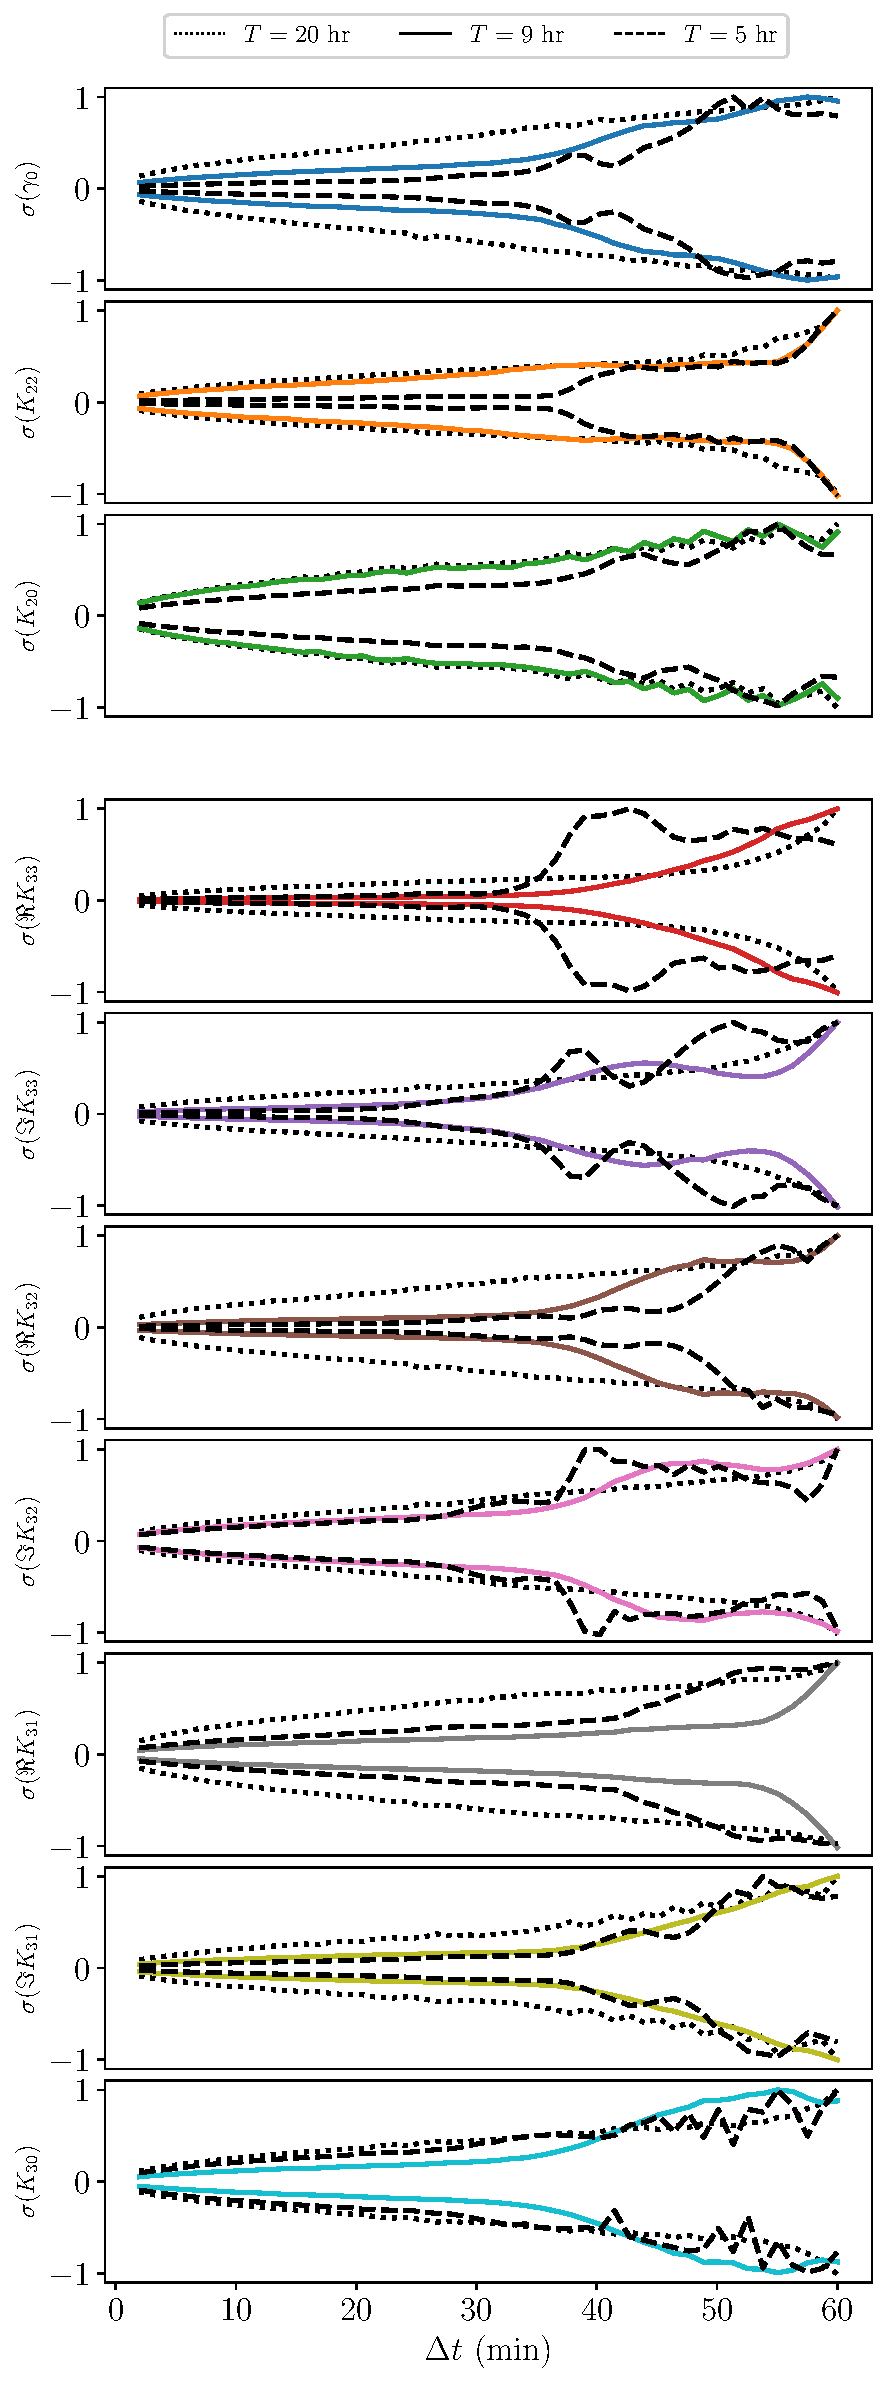
\includegraphics[width=0.48\textwidth]{figs/cad-period.pdf}\hfill
%   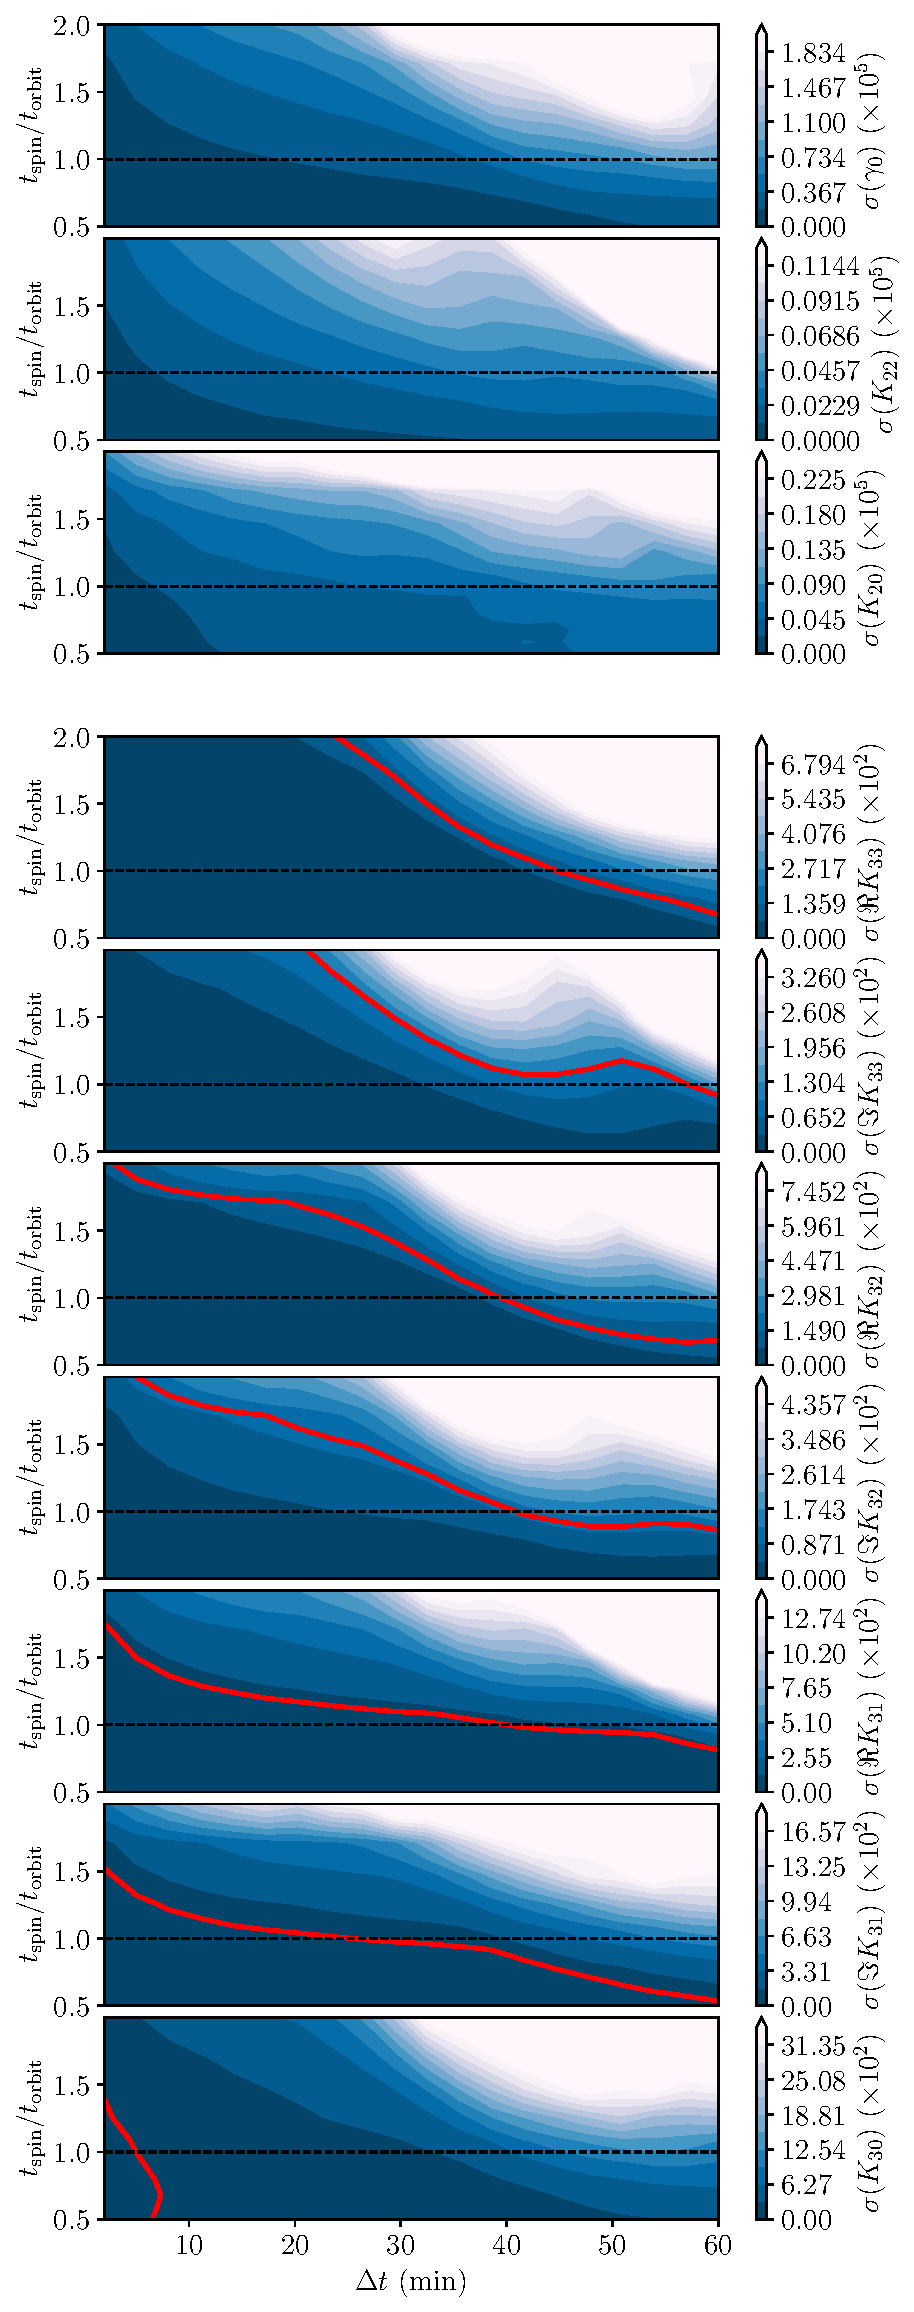
\includegraphics[width=0.48\textwidth]{figs/cad-speed.pdf}
%   \caption{Contour plots showing posterior uncertainties as a function of cadence $\Delta t$ and dynamical time scales for the encounter: rotational period $P_\omega$ (\textit{left}) and the relative speed of the orbit (\textit{right}; see text for a definition). The reference values of $P_\omega=9$ hr and $t_\text{spin}/t_\text{orbit}=1$ are shown as dotted lines. The solid (dotted) red line represents the $\sigma_\rho / \rho = 100\%$ (20\%) threshold. Cadence cut-off depends strongly on both $P_\text{omega}$ and $t_\text{spin}/t_\text{orbit}=1$.}
%   \label{fig:cad-contour}
% \end{figure*}

% Figure \ref{fig:cad-contour} demonstrates that large rotational period produces high $T_\text{cad}$. The dependence on $P_\omega$ agrees with the fact that large rotational periods for fixed cadence lead to better posterior uncertainty, discussed in section \ref{sec:scan-period}. The figure also demonstrates that for large $P_\omega$, $T_\text{cad}$ depends less strongly on $P_\text{omega}$ and may even reverse its dependence such that increasing $P_\text{omega}$ decreases $T_\text{omega}$. In all cases except $\Re K_{33}$, at least constant-$\sigma(K_{\ell m})$ contour is seen to curve back such that $\Delta t$ decreases as a function of $P_\text{omega}$ for large $P_\text{omega}$. In these regions the cadence cut-off also dulls, as shown by the spreading of the constant-$\sigma(K_{\ell m})$ contours in this region.

%  The relative orbit speed $t_\text{spin} / t_\text{orbit}$ was defined by un-physically increasing or decreasing the time at which the asteroid moved through the orbit determined by the equations of motion (but leaving the orbit shape unchanged). The equations of motion affecting the orientation and spin of the asteroid however were unaffected. $t_\text{spin} / t_\text{orbit} > 1$ corresponds to a faster orbit, and $t_\text{spin} / t_\text{orbit} < 1$ corresponds to a slower orbit. With this unphysical process, we isolate the effect of the amount of time spent near perigee on posterior uncertainty, without inheriting additional affects that would have been caused by the orbit changing shape.

% The right panel of figure \ref{fig:cad-contour} shows a stronger and more monotonic dependence of $T_\text{cad}$ on $t_\text{spin} / t_\text{orbit}$. It appears that even slightly slower orbits sharply increases $T_\text{cad}$. This effect is both due to the asteroid spending greater time in the high-torque, near-perigee region, and the larger data set that can be collected for slow orbits. However, if the orbit speed is changed by adjusting its parameters ($v_\infty$, $r_p$) or the central body mass $\mu_\mathcal{B}$, then the orbit shape will also change. This induces other effects studied in the main text and will complicate the trend observed here. Unlike the $P_\omega$ case, the cadence cut-off does not visibly broaden as a function of $t_\text{spin} / t_\text{orbit}$. It appears that the increased orbit speed merely shifts $T_\text{cad}$ rather than changing its sharpness.




\section{Animated density distributions}

This appendix contains animations to better display the density distributions shown in the main text. Each frame represents a cross section perpendicular to the $\unit z$-axis, starting with negative $z$ and ending with positive $z$. All densities are divided by the mean asteroid density.

\begin{figure*}
  \textbf{Please see the published version of the paper for these animations, or find them online at the following links.}

  \href{https://github.com/jack-dinsmore/asteroid-tidal-torque/tree/main/paper/gifs/asym-fe-d.mp4}{FE asymmetric density} \hfill
  \href{https://github.com/jack-dinsmore/asteroid-tidal-torque/tree/main/paper/gifs/asym-fe-s.mp4}{FE asymmetric deviation} \hfill
  \href{https://github.com/jack-dinsmore/asteroid-tidal-torque/tree/main/paper/gifs/asym-fe-u.mp4}{FE asymmetric uncertainty} \hfill
  \href{https://github.com/jack-dinsmore/asteroid-tidal-torque/tree/main/paper/gifs/asym-fe-r.mp4}{FE asymmetric significance}

  \href{https://github.com/jack-dinsmore/asteroid-tidal-torque/tree/main/paper/gifs/asym-l-d.mp4}{Lumpy asymmetric density} \hfill
  \href{https://github.com/jack-dinsmore/asteroid-tidal-torque/tree/main/paper/gifs/asym-l-s.mp4}{Lumpy asymmetric deviation} \hfill
  \href{https://github.com/jack-dinsmore/asteroid-tidal-torque/tree/main/paper/gifs/asym-l-u.mp4}{Lumpy asymmetric uncertainty} \hfill
  \href{https://github.com/jack-dinsmore/asteroid-tidal-torque/tree/main/paper/gifs/asym-l-r.mp4}{Lumpy asymmetric significance}

  \href{https://github.com/jack-dinsmore/asteroid-tidal-torque/tree/main/paper/gifs/sym-fe-d.mp4}{FE symmetric density} \hfill
  \href{https://github.com/jack-dinsmore/asteroid-tidal-torque/tree/main/paper/gifs/sym-fe-s.mp4}{FE symmetric deviation} \hfill
  \href{https://github.com/jack-dinsmore/asteroid-tidal-torque/tree/main/paper/gifs/sym-fe-u.mp4}{FE symmetric uncertainty} \hfill
  \href{https://github.com/jack-dinsmore/asteroid-tidal-torque/tree/main/paper/gifs/sym-fe-r.mp4}{FE symmetric significance}

  \href{https://github.com/jack-dinsmore/asteroid-tidal-torque/tree/main/paper/gifs/sym-l-d.mp4}{Lumpy symmetric density} \hfill
  \href{https://github.com/jack-dinsmore/asteroid-tidal-torque/tree/main/paper/gifs/sym-l-s.mp4}{Lumpy symmetric deviation} \hfill
  \href{https://github.com/jack-dinsmore/asteroid-tidal-torque/tree/main/paper/gifs/sym-l-u.mp4}{Lumpy symmetric uncertainty} \hfill
  \href{https://github.com/jack-dinsmore/asteroid-tidal-torque/tree/main/paper/gifs/sym-l-r.mp4}{Lumpy symmetric significance}

  \caption{Density distributions extracted via the finite element model for the asymmetric (\textit{top two rows}) and symmetric (\textit{bottom two rows}) reference asteroids. The finite element model (\textit{first and third rows}) and the lumpy model (\textit{second and fourth rows}) are employed. From left to right, the densities, deviations from the true density, uncertainties, and significance of the deviations are plotted. Animated form of figure \ref{fig:den-uniform}.}
  \label{fig:animated-uniform}
\end{figure*}

\begin{figure*}
  \textbf{Please see the published version of the paper for these animations, or find them online at the following links.}

  \href{https://github.com/jack-dinsmore/asteroid-tidal-torque/tree/main/paper/gifs/move-fe-d.mp4}{FE density} \hfill
  \href{https://github.com/jack-dinsmore/asteroid-tidal-torque/tree/main/paper/gifs/move-fe-s.mp4}{FE deviation} \hfill
  \href{https://github.com/jack-dinsmore/asteroid-tidal-torque/tree/main/paper/gifs/move-fe-u.mp4}{FE uncertainty} \hfill
  \href{https://github.com/jack-dinsmore/asteroid-tidal-torque/tree/main/paper/gifs/move-fe-r.mp4}{FE significance}

  \href{https://github.com/jack-dinsmore/asteroid-tidal-torque/tree/main/paper/gifs/move-l-d.mp4}{Lumpy density} \hfill
  \href{https://github.com/jack-dinsmore/asteroid-tidal-torque/tree/main/paper/gifs/move-l-s.mp4}{Lumpy deviation} \hfill
  \href{https://github.com/jack-dinsmore/asteroid-tidal-torque/tree/main/paper/gifs/move-l-u.mp4}{Lumpy uncertainty} \hfill
  \href{https://github.com/jack-dinsmore/asteroid-tidal-torque/tree/main/paper/gifs/move-l-r.mp4}{Lumpy significance}

  \caption{Density distributions extracted via the finite-element (\textit{top}) and lumpy (\textit{bottom}) models for an asteroid with an off-center core. From left to right, the densities, deviations from the true density, uncertainties, and significance of the deviations are plotted. Animated form of figure \ref{fig:den-move}.}
  \label{fig:animated-move}
\end{figure*}

\begin{figure*}
  \textbf{Please see the published version of the paper for these animations, or find them online at the following links.}

  \href{https://github.com/jack-dinsmore/asteroid-tidal-torque/tree/main/paper/gifs/sph-3-fe-d.mp4}{FE density} \hfill
  \href{https://github.com/jack-dinsmore/asteroid-tidal-torque/tree/main/paper/gifs/sph-3-fe-s.mp4}{FE deviation} \hfill
  \href{https://github.com/jack-dinsmore/asteroid-tidal-torque/tree/main/paper/gifs/sph-3-fe-u.mp4}{FE uncertainty} \hfill
  \href{https://github.com/jack-dinsmore/asteroid-tidal-torque/tree/main/paper/gifs/sph-3-fe-r.mp4}{FE significance}

  \href{https://github.com/jack-dinsmore/asteroid-tidal-torque/tree/main/paper/gifs/sph-3-l-d.mp4}{Lumpy density} \hfill
  \href{https://github.com/jack-dinsmore/asteroid-tidal-torque/tree/main/paper/gifs/sph-3-l-s.mp4}{Lumpy deviation} \hfill
  \href{https://github.com/jack-dinsmore/asteroid-tidal-torque/tree/main/paper/gifs/sph-3-l-u.mp4}{Lumpy uncertainty} \hfill
  \href{https://github.com/jack-dinsmore/asteroid-tidal-torque/tree/main/paper/gifs/sph-3-l-r.mp4}{Lumpy significance}

  \caption{Density distributions extracted via the finite-element (\textit{top}) and lumpy (\textit{bottom}) models for an asteroid with a centred core. From left to right, the densities, deviations from the true density, uncertainties, and significance of the deviations are plotted. Animated form of figure \ref{fig:den-sph}.}
  \label{fig:animated-sph}
\end{figure*}

\begin{figure*}
  \textbf{Please see the published version of the paper for these animations, or find them online at the following links.}

  \href{https://github.com/jack-dinsmore/asteroid-tidal-torque/tree/main/paper/gifs/double-fe-d.mp4}{FE density} \hfill
  \href{https://github.com/jack-dinsmore/asteroid-tidal-torque/tree/main/paper/gifs/double-fe-s.mp4}{FE deviation} \hfill
  \href{https://github.com/jack-dinsmore/asteroid-tidal-torque/tree/main/paper/gifs/double-fe-u.mp4}{FE uncertainty} \hfill
  \href{https://github.com/jack-dinsmore/asteroid-tidal-torque/tree/main/paper/gifs/double-fe-r.mp4}{FE significance}

  \href{https://github.com/jack-dinsmore/asteroid-tidal-torque/tree/main/paper/gifs/double-l-d.mp4}{Lumpy density} \hfill
  \href{https://github.com/jack-dinsmore/asteroid-tidal-torque/tree/main/paper/gifs/double-l-s.mp4}{Lumpy deviation} \hfill
  \href{https://github.com/jack-dinsmore/asteroid-tidal-torque/tree/main/paper/gifs/double-l-u.mp4}{Lumpy uncertainty} \hfill
  \href{https://github.com/jack-dinsmore/asteroid-tidal-torque/tree/main/paper/gifs/double-l-r.mp4}{Lumpy significance}

  \caption{Density distributions extracted via the finite-element (\textit{top}) and the two-lump lumpy (\textit{bottom}) models for an asteroid with two counterbalancing cores. From left to right, the densities, deviations from the true density, uncertainties, and significance of the deviations are plotted. Animated form of figure \ref{fig:den-double}.}
  \label{fig:animated-double}
\end{figure*}


%%%%%%%%%%%%%%%%%%%%%%%%%%%%%%%%%%%%%%%%%%%%%%%%%%

\bsp	% typesetting comment
\label{lastpage}
\end{document}